% Based on format by Jos� Koiller

%% Use the first of the following lines during production to
%% easily spot "overfull boxes" in the output. Use the second
%% line for the final version.
% \documentclass[12pt,draft,letterpaper]{report}
\documentclass[12pt,letterpaper]{report}

\newcommand{\thesistitle}{Methods for the detection and characterization \\
                          of exoplanets and their population}
\newcommand{\thesisauthor}{Daniel Foreman-Mackey}
\newcommand{\thesisadvisor}{Professor David W. Hogg}
\newcommand{\graddate}{May 2015}

%% The following makes chapters and sections, but not subsections,
%% appear in the TOC (table of contents). Increase to 2 or 3 to
%% make subsections or subsubsections appear, respectively. It seems
%% to be usual to use the "1" setting, however.
\setcounter{tocdepth}{1}

%% Sectional units up to subsubsections are numbered. To number
%% subsections, but not subsubsections, decrease this counter to 2.
\setcounter{secnumdepth}{3}

%% Page layout (customized to letter paper and NYU requirements):
\setlength{\oddsidemargin}{0in}
\setlength{\textwidth}{6.5in}
\setlength{\topmargin}{0in}
\setlength{\headheight}{0in}
\setlength{\headsep}{0in}
\setlength{\textheight}{8.3in}
% \setlength{\footskip}{.5in}
\setlength{\skip\footins}{.3in}

\usepackage{setspace}
\singlespacing{}
% \doublespacing{}

%% This inputs your auxiliary file with \usepackage's and \newcommand's:
%% It is assumed that that file is called "definitions.tex".
\RequirePackage[displaymath, mathlines]{lineno}

\usepackage[tbtags]{amsmath}
\usepackage{amssymb}
\usepackage{amsfonts}
\usepackage{amsthm}

\usepackage{color, hyperref}
\definecolor{linkcolor}{rgb}{0,0,0.2}
\hypersetup{colorlinks=true,linkcolor=linkcolor,citecolor=linkcolor,
            filecolor=linkcolor,urlcolor=linkcolor}
\hypersetup{pageanchor=false}

\usepackage{indentfirst}
\usepackage{booktabs}
\usepackage{url}
\usepackage{multirow}
\usepackage{xspace}
\usepackage{enumitem}
\usepackage[final]{graphicx}
\usepackage{wasysym}

\usepackage{footmisc}
\usepackage{soul}

\usepackage{tikz}
\usetikzlibrary{shapes.geometric, arrows}
\usetikzlibrary{fit}

\tikzstyle{hyper} = [circle, text centered, draw=black]
\tikzstyle{param} = [circle, text centered, draw=black]
\tikzstyle{data} = [circle, text centered, draw=black, line width=2pt]
\tikzstyle{arrow} = [thick,->,>=stealth]

% Custom AAS macros:
\usepackage{aas_macros}
\usepackage{lsstdesc_macros}

% Bibliography:
\usepackage{natbib}
\bibliographystyle{apj}

% Algorithms:
\usepackage{algorithmic, algorithm}

% Thesis-specific:
\newcommand{\thesistitle}{Probabilistic analysis methods for cosmology \\
	using uncertainty-dominated photometric data}
\newcommand{\thesisauthor}{Alex I. Malz}
\newcommand{\thesisadvisor}{Professor David W. Hogg}
\newcommand{\graddate}{May 2019}

% Commands:

% General formatting:
\newcommand{\paper}{Chapter}
%\newcommand{\textul}[1]{{\underline{#1}}}
\newcommand{\mathul}[1]{\underline{#1}}
\newcommand{\enquote}[1]{{``{#1}''}}

% Foreign text:
\newcommand{\foreign}[1]{\emph{#1}}
%\newcommand{\etal}{\foreign{et\,al.}}
%\newcommand{\etc}{\foreign{etc.}}

% Project references:
\newcommand{\project}[1]{{\textsc{#1}}}
\newcommand{\lsst}{\project{LSST}}
\newcommand{\desc}{\project{LSST-DESC}}
\newcommand{\coin}{\project{COIN}}
\newcommand{\sdss}{\project{SDSS}}
\newcommand{\des}{\project{DES}}

% Code references:
\newcommand{\repo}[1]{{\texttt{#1}}}
\newcommand{\qp}{\repo{qp}}
\newcommand{\chippr}{\repo{chippr}}

% Tools:
\newcommand{\github}{\href{https://github.com}{GitHub}}
\newcommand{\python}{\textit{Python}}

% LaTeX object referencing:
\newcommand{\chapid}{no chapter}
\renewcommand{\figref}[1]{\ref{\chapid:fig:#1}}
\newcommand{\Fig}[1]{Figure~\figref{#1}}
\newcommand{\fig}[1]{\Fig{#1}}
\newcommand{\figlabel}[1]{\label{\chapid:fig:#1}}

\newcommand{\Tab}[1]{Table~\ref{\chapid:tab:#1}}
\newcommand{\tab}[1]{\Tab{#1}}
\newcommand{\tablabel}[1]{\label{\chapid:tab:#1}}

\renewcommand{\eqref}[1]{\ref{\chapid:eq:#1}}
\newcommand{\Eq}[1]{Equation~(\eqref{#1})}
\newcommand{\eq}[1]{\Eq{#1}}
\newcommand{\eqalt}[1]{Equation~\eqref{#1}}
\newcommand{\eqlabel}[1]{\label{\chapid:eq:#1}}

\newcommand{\sectionname}{Section}
\newcommand{\sectref}[1]{\ref{\chapid:sect:#1}}
\newcommand{\Sect}[1]{\sectionname~\sectref{#1}}
\newcommand{\sect}[1]{\Sect{#1}}
\newcommand{\sectalt}[1]{\sectref{#1}}
\newcommand{\App}[1]{Appendix~\sectref{#1}}
\newcommand{\app}[1]{\App{#1}}
\newcommand{\sectlabel}[1]{\label{\chapid:sect:#1}}

\newcommand{\Algo}[1]{Algorithm~\ref{\chapid:algo:#1}}
\newcommand{\algo}[1]{\Algo{#1}}
\newcommand{\algolabel}[1]{\label{\chapid:algo:#1}}

\newcommand{\chapname}{Chapter}
\newcommand{\Chap}[1]{\chapname~\ref{chap:#1}}
\newcommand{\chap}[1]{\Chap{#1}}
\newcommand{\chapalt}[1]{\ref{chap:#1}}
\newcommand{\chaplabel}[1]{\label{chap:#1}}

\newcommand{\todo}[3]{{\color{#2}\emph{#1}: #3}}
\newcommand{\aim}[1]{\todo{AIM}{red}{#1}}

\newtheorem{theorem}{Theorem}[section]
\newtheorem{proposition}[theorem]{Proposition}
\newtheorem{lemma}[theorem]{Lemma}
\newtheorem{corollary}[theorem]{Corollary}
\newtheorem{conjecture}[theorem]{Conjecture}

\theoremstyle{definition}
\newtheorem{definition}[theorem]{Definition}
\newtheorem{remark}[theorem]{Remark}
\newtheorem{example}[theorem]{Example}

% Math:
%\newcommand{\dd}{\ensuremath{\,\mathrm{d}}}
\newcommand{\bvec}[1]{{\ensuremath{\boldsymbol{#1}}}}% could change to \vec
%\newcommand{\paramvector}[1]{\bvec{#1}}
%\newcommand{\unit}[1]{\mathrm{#1}}
\newcommand{\data}{\ensuremath{\vec{d}}}% could change to bold

% Probabilities:
\newcommand{\perm}[2]{\ensuremath{_{#1}\mathrm{P}_{#2}}}
\newcommand{\comb}[2]{\ensuremath{_{#1}\mathrm{C}_{#2}}}
\newcommand{\like}{\mathscr{L}}
\newcommand{\pr}[1]{\ensuremath{p(#1)}}% could change to Prob or Pr 
\newcommand{\expect}[1]{\left<#1\right>}
\newcommand{\normal}[2]{\mathcal{N} (#1, #2)}
\newcommand{\gvn}{\mid}% could use | or \vert
\newcommand{\integral}[2]{\ensuremath{\int\ #1\ \mathrm{d} #2}}

% misc science
\newcommand{\sz}{spec-$z$}
\newcommand{\Sz}{Spec-$z$}
\newcommand{\pz}{photo-$z$}
\newcommand{\Pz}{Photo-$z$}
\newcommand{\pzpdf}{\pz\ PDF}% could change to posterior
\newcommand{\Pzpdf}{\Pz\ PDF}% could change to posterior
\newcommand{\zpdf}{redshift posterior}% could change to implicit posterior
\newcommand{\pzip}{\pz\ implicit posterior}
\newcommand{\nz}{$n(z)$}
\newcommand{\Nz}{$N(z)$}
\newcommand{\stack}{$\hat{N}(z)$}

\sloppy\sloppypar


\begin{document}

%% Produces a test "layout" page, for "debugging" purposes only.
%% Comment out for final version.
% \layout  % requires package layout (see above, on this same file)

%%%%%% Title page %%%%%%%%%%%
%% Sets page numbering to "roman style" i, ii, iii, iv, etc:
\pagenumbering{roman}
%
%% No numbering in the title page:
\thispagestyle{empty}
%
\begin{center}


    \vspace*{0.5in}
    {\large\textbf{\thesistitle}}
    \vspace{.4in}

    by
    \vspace{.4in}

    \thesisauthor{}
    \vspace{.8in}
    % \vfill

    \begin{doublespace}
        A dissertation submitted in partial fulfillment \\
        of the requirements for the degree of \\
        Doctor of Philosophy \\
        Department of Physics \\
        New York University \\
        \graddate{}
    \end{doublespace}
\end{center}
\vfill

\noindent\makebox[\textwidth]{\hfill\makebox[2.5in]{\hrulefill}}\\
\makebox[\textwidth]{\hfill\makebox[2.5in]{\hfill\thesisadvisor\hfill}}
\newpage

%%%%%%%%%%%%%% Copyright %%%%%%%%%%%%%%%%%
\vspace*{\fill}
\begin{center}
    Copyright \textcopyright\ 2015 Daniel Foreman-Mackey \\
    This work is licensed under a Creative Commons Attribution 4.0
    International License.
    \addcontentsline{toc}{section}{Copyright}
\end{center}
\vfill
\newpage

%%%%%%%%%%%%% Blank page %%%%%%%%%%%%%%%%%%
\thispagestyle{empty}
\vspace*{0in}
\newpage

%%%%%%%%%%%%%% Acknowledgements %%%%%%%%%%%%
%% Comment out the following lines if you do not want to acknowledge
%% anyone's help...
\section*{Acknowledgements}\addcontentsline{toc}{section}{Acknowledgements}
%% Write your acknowledgements in this file. If you do not want to acknowledge anyone,
%% you can delete this file and comment out the corresponding part in the "thesis.tex"
%% file.
%
I would like to acknowledge the effort put into this thesis by
myself. This work could not have been done without me.

\newpage

%%%% Abstract %%%%%%%%%%%%%%%%%%
\section*{Abstract}\addcontentsline{toc}{section}{Abstract}
The study of exoplanets has been revolutionized in recent years thanks, in
large part, to new data collected by NASA's \emph{Kepler} Mission.
The Mission has enabled the discovery of thousands of planets orbiting stars
throughout the Galaxy.
These discoveries span orders of magnitude in physical parameter space but
many of the most physically interesting questions remain open.
The deepest of these questions is: how common are planetary systems like our
own Solar System?
In this dissertation, I approach this question from several different angles
and make inferences about the frequency and distribution of planets based on
the large, publicly-available datasets from the \emph{Kepler} Mission.

I develop two powerful and practical methods for mining for planetary transit
signals in the hundreds of thousands of stellar light curves measured by
\emph{Kepler}.
The first method is designed to find planets using the data from the
\emph{K2} phase of the Mission where systematics introduced by the instrument
dominate the measurements.
Applying this method to the first publicly available dataset from \emph{K2},
Campaign 1, I published more than thirty new exoplanet candidates.
The second transit search technique is designed to find transits of planets
with orbital periods longer than the four year baseline of the \emph{Kepler}
Mission.
These are interesting planets because they are expected to have the largest
dynamical influence on the formation and evolution of their planetary systems
but, to date, no systematic search for these signals has been published.
I demonstrate that this method is robust and tractable and make predictions
for the planet yields in the \emph{Kepler} dataset.

I derive a general framework for making justified probabilistic inferences
about the population of planets based on noisy and incomplete catalogs of
exoplanet measurements.
Applying this to a previously published catalog of exoplanets orbiting stars
like our Sun, I measure the joint period--radius distribution of these
planets taking into account survey selection effects and the large
measurement uncertainties.
Despite the fact that this catalog includes no true Earth analogs, I use the
detected systems and weak smoothness assumptions about the underlying
distribution to make a probabilistic estimate of the frequency of Earth-like
planets.

\newpage

%%%% Table of Contents %%%%%%%%%%%%
\tableofcontents

%%%%% List of Figures %%%%%%%%%%%%%
%% Comment out the following two lines if your thesis does not
%% contain any figures. The list of figures contains only
%% those figures included withing the "figure" environment.
\listoffigures\addcontentsline{toc}{section}{List of Figures}
\newpage

%%%%% List of Tables %%%%%%%%%%%%%
%% Comment out the following two lines if your thesis does not
%% contain any tables. The list of tables contains only
%% those tables included withing the "table" environment.
\listoftables\addcontentsline{toc}{section}{List of Tables}
\newpage

%%%%% Body of thesis starts %%%%%%%%%%%%
\pagenumbering{arabic}

%% Introduction. If your thesis has no introduction, or chapter 1 is
%% meant to be the introduction, then comment out the lines below.
\chapter*{Introduction}\addcontentsline{toc}{chapter}{Introduction}
\chapter*{Introduction}\addcontentsline{toc}{chapter}{Introduction}

%[Why do we need redshifts? cosmology problems and galaxy evolution, use as distance proxy via Hubble law]

Photometric redshift (\pz) estimation has been a staple of studies of galaxy evolution, large-scale structure, and cosmology since its conception decades ago \citep{Baum1962}.  
An extremely coarse spectrum in the form of photometry in a handful of broadband filters can be an effective substitute for the time- and photon-intensive process of obtaining a spectroscopic redshift (\sz), a procedure that may only be applied to relatively bright galaxies.  
Once the photometric colors are calibrated against either a library of spectral energy distribution (SED) templates or a data set of spectra for galaxies with known redshifts, a correspondence between photometric colors and redshifts may be constructed, forming a trustworthy basis for \pz\ estimation or testing.

Many more \pz s may be obtained in the time it would take to observe a smaller number of \sz s, and \pz s may be measured for galaxies too dim for accurate \sz\ confirmation, permitting the compilation of large surveys of galaxy redshifts spanning a broad range of redshifts and luminosities.  
\Pz s have thus enabled the era of precision cosmology, heralded by weak gravitational lensing tomography and baryon acoustic oscillation peak measurements.  
Calculations of correlation functions of cosmic shears and galaxy positions require large numbers of high-confidence redshifts of surveyed galaxies.  

However, \pz s are susceptible to inaccuracy and imprecision via a number of effects, particularly their inherent noisiness due to the coarseness of photometric filters, catastrophic errors in which galaxies of one type at one redshift are mistaken for galaxies of another type at a different redshift, and systematics introduced by observational techniques, data reduction processes, and training set limitations.  
The projection of these effects into the space of true and estimated redshifts is discussed extensively in \Chap{pzdc1}, and their impact on cosmological parameter constraints is addressed in \Chap{chippr}, and \Fig{fig:pedagogical_scatter} in particular.
Based on the goals of a photometric galaxy survey, requirements can be placed on the accuracy of \pz\ estimates.
For example, the Large Synoptic Survey Telescope (\lsst) states requirements for the main cosmological sample in the \lsst\ Science Requirements Document (SRD)\footnote{\url{https://docushare.lsstcorp.org/docushare/dsweb/Get/LPM-17}} and reproduced in \Tab{tab:lsst-srd}.

\begin{table}
	\begin{tabular}{ll}
		Number of galaxies & $\sim 10^{7}$\\
		Root-mean-square error & $\sigma_z < 0.02 (1+z)$\\
		$3 \sigma$ catastrophic outlier rate & $< 10\%$\\
		bias & $< 0.003$
	\end{tabular}
\tablabel{tab:lsstsrd}
\caption{\Pz\ requirements for \lsst\ cosmology.}
\end{table}

In addition to these limitations in accuracy, there is also the matter of uncertainty quantification; \pz s are often reported with presumed-Gaussian error bars derived without inclusion of all systematic errors, including the different selection effects between the photometric color- or magnitude-spaces of galaxies for which \pz s are desired and galaxies with \sz s are used to calibrate \pz\ estimators.
An example of the impact of this selection bias in the context of \citep[\project{zCOSMOS}][]{lilly_zcosmos_2009} and \citep[\project{COSMOS}][]{laigle_cosmos2015_2016} is shown in \Fig{fig:selection-bias}.
This lack of support can bias one-point statistics of the affected galaxy populations \citep{moresco_spot_2013}, and elaborate procedures for compensating for such bias have been developed in the context of two-point statistics of galaxy redshifts \citep{mandelbaum_precision_2008}.

\begin{figure*}
	\begin{center}
		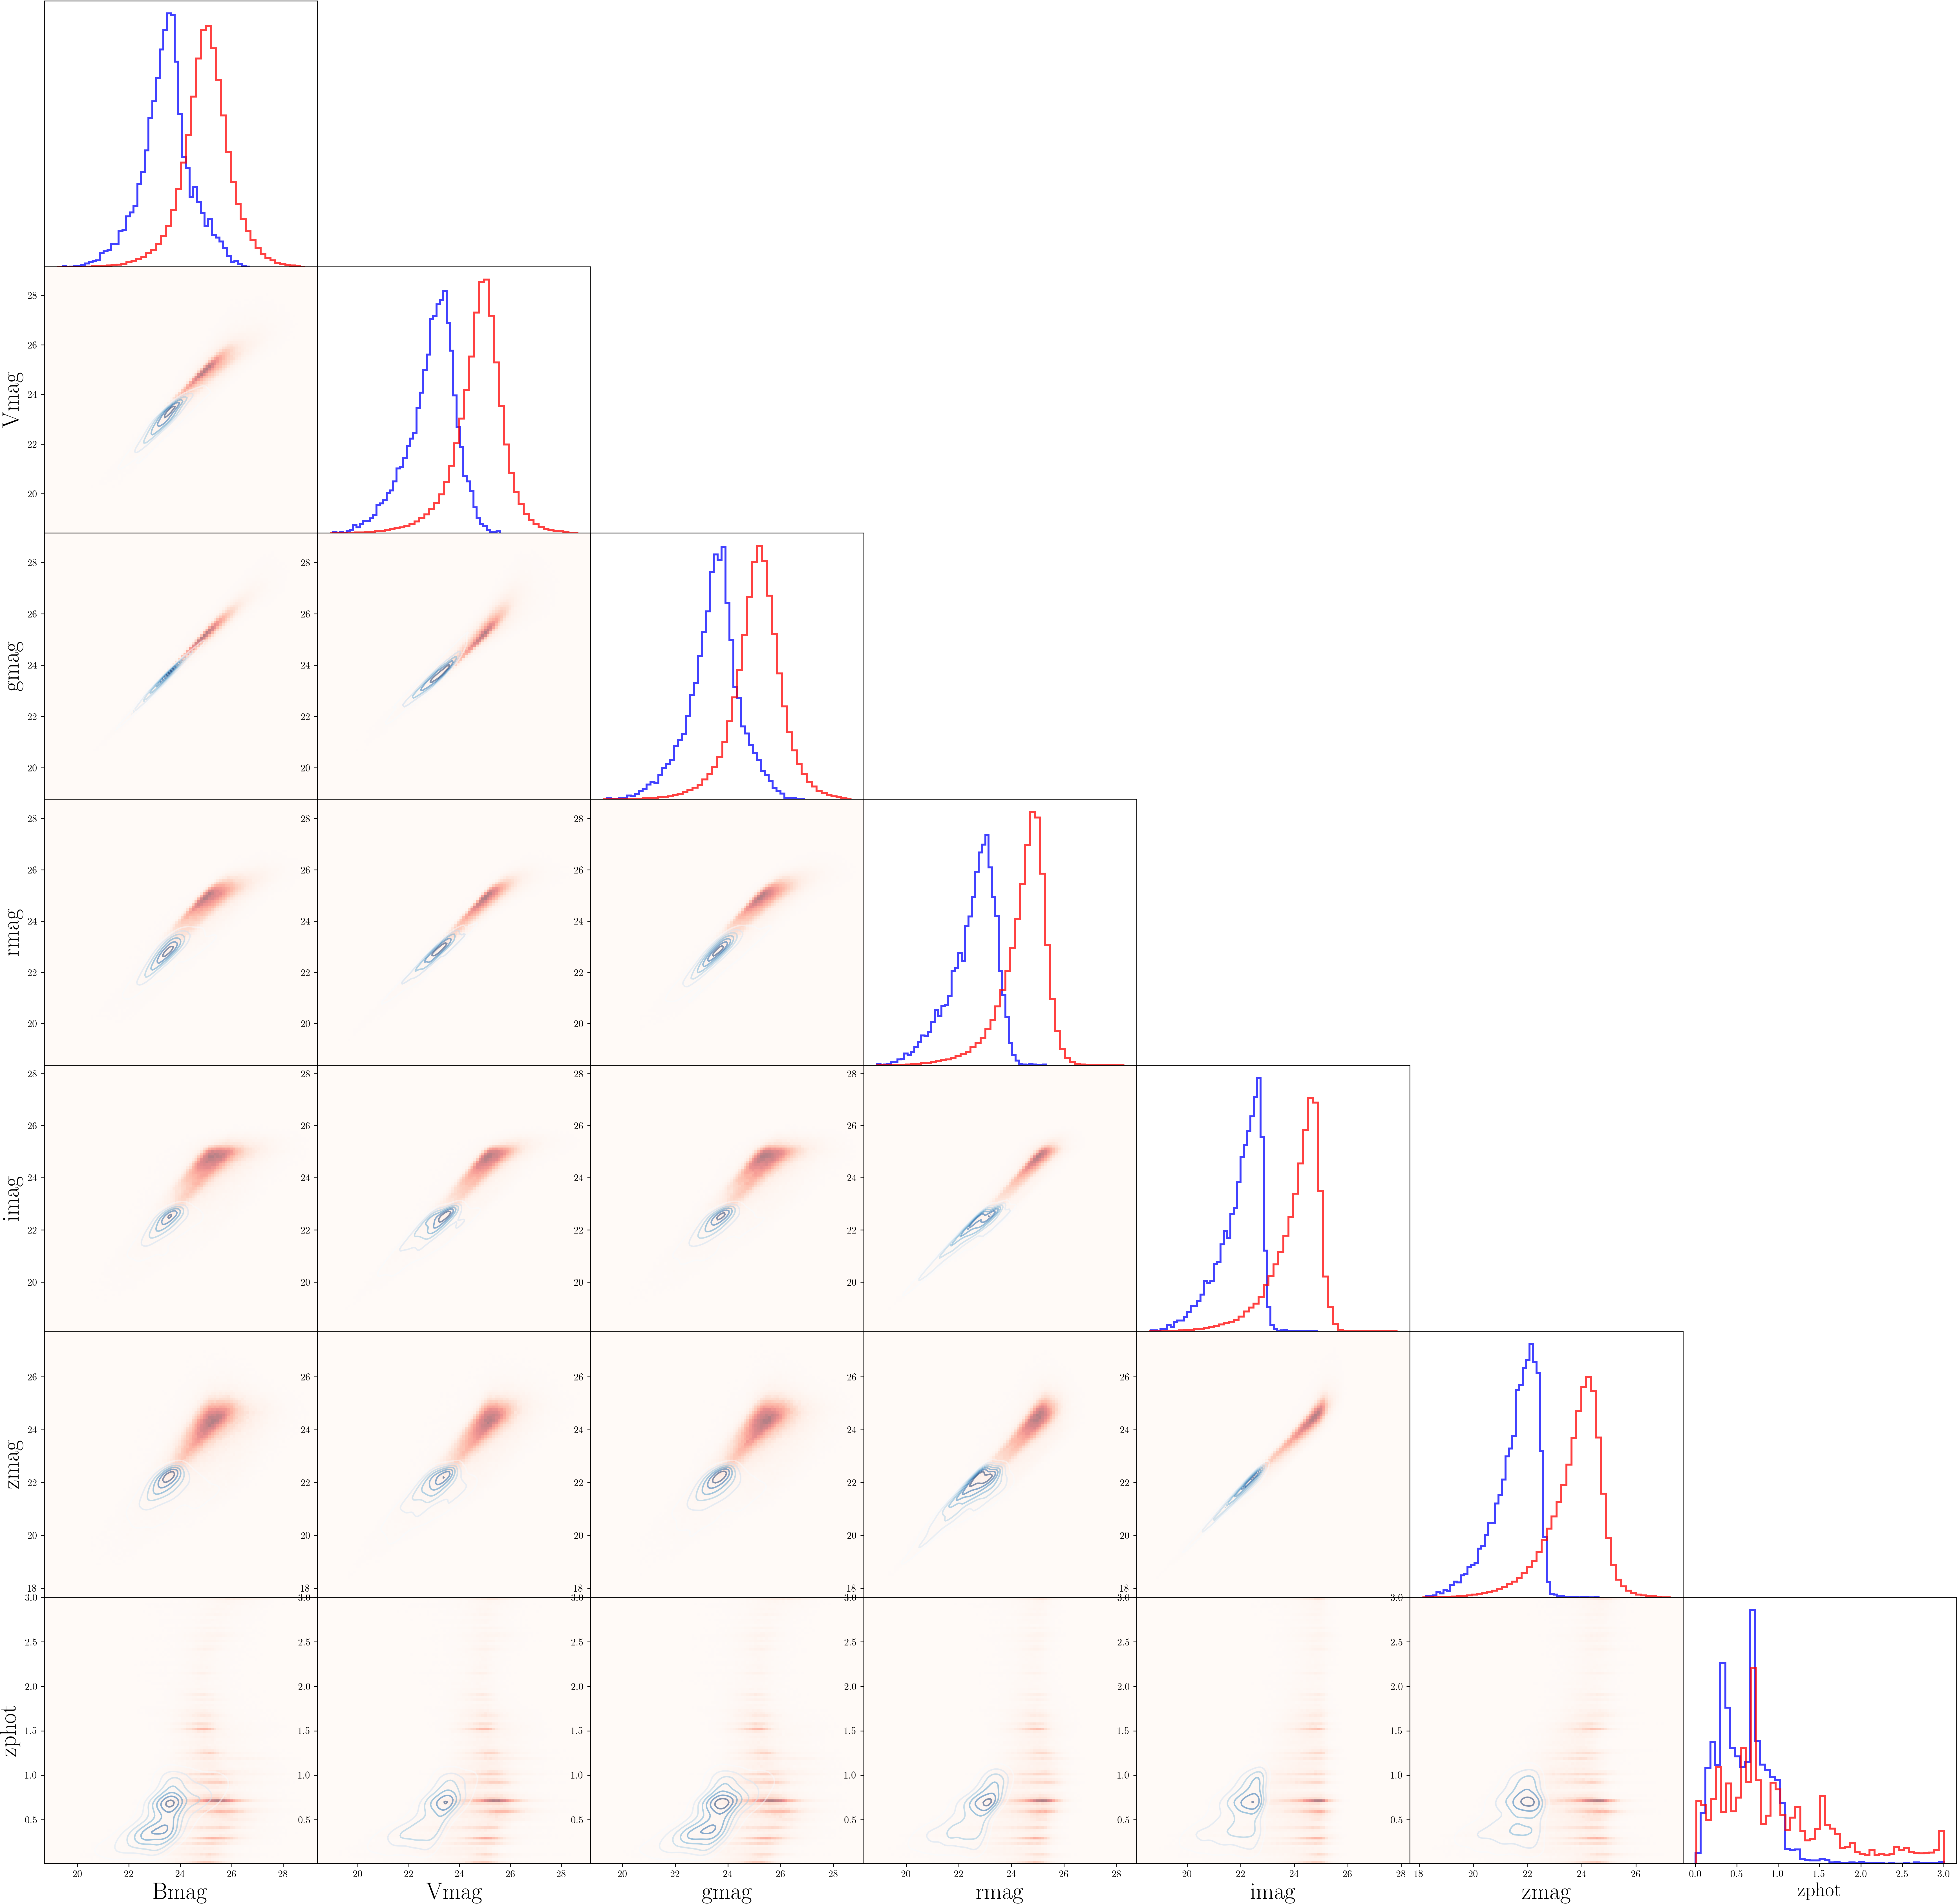
\includegraphics[width=0.99\textwidth]{figures/intro/big_corner_coarse.png}
		\caption{
			The distributions of magnitudes and the provided photometric redshift estimate for the galaxies with complete photometric data in \project{zCOSMOS} ($8,826$ galaxies; blue) and \project{COSMOS} ($395,019$ galaxies; red).
			It is evident that the sample for which spectra were unavailable is not well-supported by the sample for which spectra were obtained, which was used to calibrate the spectroscopically unconfirmed set.
		}
		\figlabel{fig:selection-bias}
	\end{center}
\end{figure*}

%Several factors contribute to photometric redshifts' intrinsic scatter.  
%Distant galaxies are dimmer compared to galaxies of identical luminosity that are closer, driving up photometric errors in flux-limited surveys.  
%The nature of the galaxy sample at higher redshifts also changes, meaning the generation of the photometric redshift posterior based on an a locally-calibrated SED template library or spectroscopically-confirmed training set is more likely to be inappropriate, leading to broader features.  
%In general, the galaxies that could not have been observed spectroscopically will have different and noisier photo-$z$ likelihoods than those that could fall into a spectroscopic training set (or spectroscopically derived template library).  
%This effect may be stronger for high-redshift galaxies.  

Once propagated through the calculations of correlation functions of cosmic shear and galaxy positions, these sources of \pz\ errors are not insignificant contributors to the total uncertainties reported on cosmological parameters.
As other systematic errors have been resolved, the uncertainties associated with \pz s have come to dominate the uncertainties on estimates of cosmological parameters made by current surveys such as \des \citep{hoyle_dark_2017}.

Much effort has been dedicated to improving \pz s, though they are still most commonly obtained by a maximum likelihood estimator (MLE) based on libraries of galaxy SED templates, with conservative approaches to error estimation.  
Recent advances have focused on identifying and removing catastrophic outliers when using \pz s for 
inference \citep{Gorecki2014}.  
Sophisticated Bayesian techniques and cutting-edge machine learning methods have been employed to improve precision \citep{Carliles2010} and accuracy \citep{Sadeh2015}. 

An alternative to point estimation of \pz s is redshift probability distribution function (PDF) estimation that reports the probability $p(z)$ over all possible redshifts for every galaxy rather than an MLE (with or without presumed Gaussian error bars) \citep{Koo1999}.  
This option is favorable because it contains more potentially useful information about the uncertainty on each galaxy's redshift than a point estimate, incorporating notions of precision, accuracy, and systematic errors.
However, denoting \pzpdf s as ``$\pr{z}$'' is an abuse of notation, as it does not adequately convey what information is being used to constrain the redshift $z$; \pzpdf s are \textit{posterior} PDFs, conditioned on the photometric data and prior knowledge, as is covered in detail in \Chap{pedant}, as well as \Chap{chippr} and \Chap{pzdc1}.

\aim{what interesting problems/opportunities are the context for my work?  (drawing conclusions about the universe from vast quantities of uncertainty-dominated, limitations of photometry lead to methodological challenges, what was tried so far and why isn't it good enough)}

\aim{what science can be done with that opportunity? (cosmology, and then some! the interesting problems are in testing LCDM, GR, inflation, also galaxy evolution)}

\Pzpdf s have been produced by completed surveys \citep{Hildebrandt2012, Sheldon2012} and will be produced by ongoing and upcoming surveys \citep{LSSTScienceCollaboration2009, CarrascoKind2014a, Bonnett2015, Masters2015}.  
\Pzpdf s are not without their own weaknesses, however, including the resources necessary to calculate and record them for large galaxy surveys \citep{CarrascoKind2014} and the method used to derive them.  
The most important of these issues, however, is that use of them in the literature is inconsistent at best and incorrect at worst.  
The most common application of \pzpdf s is their use in estimating \Nz, the distribution of redshifts of a sample of galaxies, a quantity essential to the calculation of the power spectra of weak gravitational lensing and large-scale structure that are used to constrain the parameters of cosmological models.
\aim{Provide equations/citations for the use of \Nz\ in cosmology.}

If the true redshifts $\{z_{j'}\}$ were known, the redshift probabilities would be delta functions $\{\delta(z, z'_{j})\}$ centered at the true redshift, and the redshift distribution could be approximated by a histogram or other interpolation of the delta functions $\{\delta(z, z'_{j})\}$.
When \pzpdf s are available instead of true redshifts, the simplest approach reduces them to point estimates of redshift by using $\delta(z, \hat{z}_{j})$ in place of $\delta(z, z'_{j})$, where $\hat{z}_{j}$ may be the mode (maximum) of the \pzpdf, though there are other, more principled options \citep{tanaka_photometric_2018-1}.
However, it is more common at this point to calculate the mathematically invalid but conceptually simple \textit{stacked estimator} of the redshift density function \citep{Lima2008}, 
\begin{align}
\eqlabel{eqn:stack}
\hat{n}(z) &= \frac{1}{\ntot} \sum_{i = 0}^{\ntot} \pr{z_{i}}
\end{align}
for a sample of $\ntot$ galaxies $i$, or, equivalently, the redshift distribution function $\hat{N}(z) = \ntot \hat{n}(z)$.

In \Chap{pedant}, I address the question of how a blatantly incorrect estimator of the redshift distribution could become widely accepted by otherwise clever astrophysicists.
I approach the problem from a mathematically rigorous perspective to identify the assumptions necessary for the stacked estimator to approach the true \Nz and note that because those assumptions will not hold for future surveys, including \lsst, we must use an alternative estimator that self-consistently propagates redshift uncertainty.

I go on to present one such an alternative to stacking, the Cosmological Hierarchical Inference with Probabilistic Photometric Redshifts (\Chippr), in \Chap{chippr}.
\Chippr\ is a probabilistic graphical model (PGM) that encapsulates the causal relationships between the redshift distribution, samples of individual galaxy redshifts, and photometric data.
I also present the \chippr\ code that implements the \Chippr\ model and includes a comprehensive suite of tools for testing arbitrarily realistic mock \pzpdf\ catalogs.

\aim{Hogg says ``I think it would be good to talk a little quantitatively about where people need to know N(z) and other one-point statistics, and how much they will get various things wrong if they don't know these correctly. 
	And situate that discussion within the current context of cosmological parameter estimation and precision cosmology.''}

In order for the approach proposed in \Chap{chippr} to be applied, there must be a \pzpdf\ catalog, yet many techniques to obtain \pzpdf s have been proposed and tested in the literature without clear indications that one is superior to all others.  
An extension of the Bayesian photometric redshift (BPZ) method of \citet{Benitez2000} that produces posterior probability distributions (as opposed to a selection of local maxima) from an SED template library has been employed \citep{Hildebrandt2012, Kelly2014, Lopez-Sanjuan2015}.  
\Pzpdf s have also been obtained by a variety of trustworthy data-driven approaches in the literature: $k$-nearest neighbor algorithms with \citep{Ball2008} and without \citep{Sheldon2012} inclusion of photometric measurement errors, neural networks \citep{Bonnett2015a}, self-organizing maps \citep{CarrascoKind2014a}, and prediction tree and random forest classification techniques \citep{Carliles2010, CarrascoKind2013}.  
(The approaches of fitting to a training set and fitting to a template library are related to one another by \citet{Budavari2009}.)  
Hierarchical inference has also been applied to calculate \pzpdf s simultaneously with the overall redshift distribution function \citep{Leistedt2016}.  
Of course, this brief review does not cover all ways to obtain \pzpdf s; many more may be found in the literature, along with comparisons thereof \citep{Hildebrandt2010, Dahlen2013, Sanchez2013, Bonnett2015}.
Some current work aims to vet \pzpdf\ generation methods \citep{Wittman2016}.
\aim{Also cite the HSC comparison of \pzpdf\ methods, and maybe the DES one even though it only compares two.}
\Chap{pzdc1} details the comparative study of Schmidt, Malz, and Soo, et al. (in review) but goes beyond the scope of previous attempts to identify the best \pzpdf\ technique by critiquing the evaluation criteria themselves from a mathematically rigorous perspective.
\aim{Make this a real citation with a link to the paper.}

In the absence of an obvious best choice for the method used to derive \pzpdf s, \lsst\ has planned to provide \pzpdf s obtained by a number of promising methods rather than choosing one, effectively hedging their bets on which may ultimately prevail.
This goal of storing multiple \pzpdf s, however, must be accomplished without exceeding the available data storage capacity of the survey nor compromising the integrity of subsequent science applications due to loss of information in the compression and reconstruction schemes.
\Chap{qp} approaches the problem of choosing how best to store \pzpdf s such that the results of multiple \pzpdf\ techniques may be available to the scientific community, focusing in particular on the number of stored parameters under different possible parameterizations of stored \pzpdf s.

\aim{Update this paragraph for the existence of \Chap{pedant}.}
\Chap{chippr} presents a mathematically rigorous methodology for inferring \Nz\ from a catalog of \pzpdf s, including the effect of incorrectly inferred \Nz\ on cosmological parameter estimates.
\Chap{pzdc1} contains a comprehensive comparison of twelve approaches to probabilistic photometric redshift estimation, presenting novel discoveries of the impact of the assumptions implicit to the method by which the redshift probabilities are derived and the limitations of established performance metrics of such probabilistic data products in assessing the quality of the procedures for deriving them.
I also address in \Chap{qp} a practical concern regarding how redshift probabilities are to actually be used, answering the question of how probabilistic data products should be stored and delivered to users in order to ensure that scientific progress can be made, as well as how to go about answering that question for a generic science application.

\aim{did I produce anything of value? if there's a product, maybe cite it here?}

\chapname~\chapalt{chippr} has been presented at numerous conferences but remains an unpublished, public draft accompanied by a public code.
\chapname~\chapalt{pzdc1} is currently under \desc\ internal review, with intended submission to MNRAS.
\chapname~\chapalt{qp} has been refereed and published in AJ, with code published on Zenodo.
Here, I describe my specific contributions to each \chapname and acknowledge the contributions of my co-authors:
\begin{enumerate}

{\item For \chap{chippr}, I led the development, implementation, and validation of CHIPPR initially under the supervision of David Hogg (NYU) and later continued to work on all three aspects of the project under the supervision of Phil Marshall (SLAC).
	I developed the mathematical formalism in consultation with Phil Marshall (SLAC).}

{\item For \chap{pzdc1}, I led the choice, evaluation, and interpretation of the comparison metrics, and I devised and implemented the \texttt{trainZ} technique of \pzpdf\ estimation.
	I wrote the paper in collaboration with Sam Schmidt (UC Davis), John Soo (U. of Science Malaysia), and the \Pz\ Working Group of the \desc.  
	The mock data was produced and validated by Alex Abate (Dia\&Co), Sam Schmidt (UC Davis), Eve Kovacs (Argonne), Joe DeRose (Stanford), Risa Wechsler (Stanford), Tina Peters (Toronto).
	The experimental design was chosen by Ofer Lahav (UCL), Jeff Newman (Pitt), Sam Schmidt (UC Davis), and Tony Tyson (UC Davis).
	I chose the metrics to test with input from Jeff Newman (Pitt) and Ann Lee (CMU).
	I worked together with Rongpu Zhou (Pitt), Bryce Kalmbach (UW), Kartik Iyer (Rutgers), Sam Schmidt (UC Davis), and Chris Morrison (UW) to implement the comparison metrics and run them on the results of different \pzpdf\ codes.
	The \pzpdf\ codes themselves were written and/or run by Ibrahim Almosallam (King Abdulaziz City for Science and Technology), Massimo Brescia (INAF-Capodimonte), Stefano Cavuoti (University Federico II), Johann Cohen-Tanugi (Universit\'e de Montpellier),  Andy Connolly (UW), Peter Freeman (CMU), Melissa Graham (UW), Rafael Izbicki (Federal University of Sao Carlos), Matt Jarvis (Oxford; University of the Western Cape), Ann Lee (CMU), Giuseppe Longo (University Federico II), Erfan Nourbakhsh (UC Davis), Eric Nuss (Universit\'e de Montpellier), Taylor Pospisil (CMU), Cecile Roucelle (U Clermont-Ferrand), and Hugo Tranin (Universit\'e de Montpellier).
	The paper is intended for submission to MNRAS but is still under internal review by \desc\ members Mike Troxel (Duke), Markus Michael Rau (CMU), and Daniel Gruen (Stanford).}

{\item For \chap{qp}, I devised the idea for the project, conducted the investigation, wrote and validated the \texttt{qp} code, and wrote the paper under the supervision of Phil Marshall (SLAC), with contributions to the mock data production by Sam Schmidt (UC Davis), Melissa Graham (UW), Joe DeRose (Stanford), and Risa Wechsler (Stanford).
	The paper was internally reviewed by \desc\ members Chad Schafer (CMU), Boris Leistedt (NYU), and Chris Morrison (UW).}

\end{enumerate}


\renewcommand{\chapid}{emcee}

% Chapter specific commands:
\newcommand{\thisplain}{emcee}
\newcommand{\this}{\project{\thisplain}}
\newcommand{\license}{MIT License}
\newcommand{\Python}{\project{Python}}
\newcommand{\numpy}{\project{numpy}}
\newcommand{\Ubuntu}{\project{Ubuntu}}
\newcommand{\github}{\project{GitHub}}
\newcommand{\pip}{\project{pip}}
\newcommand{\acor}{\project{acor}}
\defcitealias{Goodman:2010}{GW10}

% Math:
\newcommand{\model}{\ensuremath{\vector{\Theta}}}
\newcommand{\data}{\ensuremath{\vector{D}}}
\newcommand{\nuisance}{\ensuremath{\vector{\alpha}}}
\newcommand{\link}{\ensuremath{X}}
\newcommand{\ensemble}{S}
\newcommand{\colorens}[1]{\ensemble^{(#1)}}
\newcommand{\red}{\colorens{0}}
\newcommand{\blue}{\colorens{1}}
\renewcommand{\vector}[1]{#1}
\renewcommand{\matrix}[1]{#1}

\chapter{\this: The MCMC Hammer\chaplabel{emcee}}

This \paper\ is joint work with David~W.~Hogg (NYU), Jonathan~Goodman (NYU),
and Dustin~Lang (Princeton/CMU) published in \emph{Publications of the
Astronomical Society of the Pacific} as \citet{Foreman-Mackey:2013}.

\section{Chapter abstract}

We introduce a stable, well tested Python implementation of the affine-%
invariant ensemble sampler for Markov chain Monte Carlo (MCMC)
proposed by Goodman \& Weare (2010). The code is open source and has
already been used in several published projects in the astrophysics
literature. The algorithm behind \this\ has several advantages over
traditional MCMC sampling methods and it has excellent performance as
measured by the autocorrelation time (or function calls per independent sample).
One major advantage of the algorithm is that it requires hand-tuning of
only 1 or 2 parameters compared to $\sim N^2$ for
a traditional algorithm in an $N$-dimensional parameter space. In this
\paper, we describe the algorithm and the details of our implementation.
Exploiting the parallelism of the ensemble method,
\this\ permits \emph{any} user to take advantage of
multiple CPU cores without extra effort.  The code is available online
at \url{http://dan.iel.fm/\thisplain} under the \license.

\section{Introduction}

Probabilistic data analysis---including Bayesian inference---has
transformed scientific research in the past decade. Many of the most
significant gains have come from numerical methods for approximate
inference, especially Markov chain Monte Carlo (MCMC).  For example,
many problems in cosmology and astrophysics\footnote{The methods and
  discussion in this \paper\ have general applicability, but we will
  mostly present examples from astrophysics and cosmology, the fields
  in which we have most experience} have directly benefited from MCMC
because the models are often expensive to compute, there are many free
parameters, and the observations are usually low in signal-to-noise.

Probabilistic data analysis procedures involve computing and using
either the posterior probability density function (PDF) for the
parameters of the model or the likelihood function. In some cases it
is sufficient to find the maximum of one of these, but it is often
necessary to understand the posterior PDF in detail.  MCMC methods are
designed to sample from---and thereby provide sampling approximations
to---the posterior PDF efficiently even in parameter spaces with large
numbers of dimensions. This has proven useful in too many research
applications to list here but the results from the NASA Wilkinson
Microwave Anisotropy Probe (WMAP) cosmology mission provide a dramatic
example \citep[for example,][]{Dunkley:2005}.

Arguably the most important advantage of Bayesian data analysis is
that it is possible to \emph{marginalize} over nuisance parameters. A
nuisance parameter is one that is required in order to model the
process that generates the data, but is otherwise of little interest.
Marginalization is the process of integrating over all possible values of
the  parameter and hence propagating the effects of uncertainty about
its value into the final result.  Often we wish to marginalize over all
nuisance parameters in a model.  The exact result of marginalization
is the marginalized probability function \pr{\model | \data}
of the set (list or vector) of model parameters
\model\ given the set of observations \data
\begin{equation}
    \eqlabel{marginalization}
    \pr{\model | \data} = \int
        \pr{ \model, \nuisance | \data} \,
        \dd  \nuisance \quad,
\end{equation}
where \nuisance\ is the set (list or vector) of nuisance
parameters. Because the nuisance parameter set \nuisance\ can be very large, this
integral is often extremely daunting.  However, a
MCMC-generated sampling of values $(\model_t,\nuisance_t)$ of the
model and nuisance parameters from the joint distribution $\pr{\model,
  \nuisance | \data}$ automatically provides a sampling of values
$\model_t$ from the marginalized PDF $\pr{\model | \data}$.

In addition to the problem of marginalization, in many problems of
interest the likelihood or the prior is the result of an expensive
simulation or computation. In this regime, MCMC sampling is very
valuable, but it is even \emph{more} valuable if the MCMC algorithm is
efficient, in the sense that it does not require many function
evaluations to generate a statistically independent sample from the
posterior PDF.  The methods presented here are designed for efficiency.

Most uses of MCMC in the astrophysics literature are based on slight
modifications to the Metropolis-Hastings (M--H) method (introduced
below in \sect{algo}).  Each step in a M--H chain is proposed using a
compact proposal distribution centered on the current position of the
chain (normally a multivariate Gaussian or something similar). Since
each term in the covariance matrix of this proposal distribution is an
unspecified parameter, this method has $N\,[N+1]/2$ tuning parameters
(where $N$ is the dimension of the parameter space).  To make matters
worse, the performance of this sampler is very sensitive to these
tuning parameters and there is no fool-proof method for choosing the
values correctly. As a result, many heuristic methods have been
developed to attempt to determine the optimal parameters in a
data-driven way \citep[for
  example,][]{Gregory:2005,Dunkley:2005,Widrow:2008}. Unfortunately,
these methods all require a lengthy ``burn-in'' phase where shorter
Markov chains are sampled and the results are used to tune the
hyperparameters. This extra cost is unacceptable when the likelihood
calls are computationally expensive.

The problem with traditional sampling methods can be visualized by looking
at the simple but highly anisotropic density
\begin{equation}
    \eqlabel{anisotropic}
    p(\mathbf{x}) \propto f \left (-\frac{(x_1-x_2)^2}{2\,\epsilon}
                                        - \frac{(x_1+x_2)^2}{2} \right )
\end{equation}
which would be considered difficult (in the small-$\epsilon$ regime) for
standard MCMC algorithms. In principle, it is possible to tune the
hyperparameters of a M--H sampler to make this sampling converge quickly,
but if the dimension is large and calculating the density
is computationally expensive the tuning procedure becomes intractable.
Also, since the number of parameters scales as $\sim N^2$, this problem gets
much worse in higher dimensions.
\Eq{anisotropic} can, however, be transformed into the much easier problem of
sampling an isotropic density by an \emph{affine transformation} of the form
\begin{equation}
    y_1 = \frac{x_1-x_2}{\sqrt{\epsilon}} \, ,
        \hspace{1cm} y_2 = x_1 + x_2 \quad .
\end{equation}
This motivates affine invariance: an algorithm that is \emph{affine invariant}
performs equally well under all linear transformations; it will therefore be
insensitive to
covariances among parameters.

\citet[][hereafter \citetalias{Goodman:2010}]{Goodman:2010} proposed an affine
invariant sampling algorithm (\sect{algo}) with only two hyperparameters to be
tuned for performance. \citet{Hou:2012} were the first group to implement this
algorithm in astrophysics. The implementation presented here is
an independent effort that has already proved effective for many projects in
the astronomical
literature\footnote{\url{http://adsabs.harvard.edu/cgi-bin/nph-ref_query?bibcode=2013PASP..125..306F}}.
In what follows, we summarize the
algorithm from \citetalias{Goodman:2010} and the implementation
decisions made in \this. We also describe the small changes
that must be made to the algorithm to parallelize it.

\section{The algorithm}\sectlabel{algo}

A complete discussion of MCMC methods is beyond the scope of this \paper.
Instead, the interested reader is directed to a classic reference like
\citet{MacKay:2003} and we will summarize some key concepts below.

The general goal of MCMC algorithms is to draw $M$ samples
$\{ \model_i \}$ from
the posterior probability density
\begin{equation}
    \pr{\model, \nuisance | \data} = \frac{1}{Z}\,\pr{\model, \nuisance}
            \, \pr{\data | \model, \nuisance} \quad,
\end{equation}
where the prior distribution $\pr{\model, \nuisance}$ and the likelihood
function $\pr{\data|\model,\nuisance}$ can be relatively easily (but not
necessarily quickly) computed for any particular value of
$(\model_i, \nuisance_i)$.  The normalization $Z=\pr{\data}$ is
independent of $\model$ and $\nuisance$ once we have chosen the form of the
generative model. This means that it is possible
to sample from \pr{\model, \nuisance | \data} without computing $Z$ ---
unless one would like to compare the validity of two different generative
models. This is important because $Z$ is generally very expensive to
compute.

Once the samples
produced by MCMC are available, the marginalized constraints on $\model$
can be approximated by
the histogram of the samples projected into the parameter subspace spanned
by $\model$. In particular, this implies that the
expectation value of a function of the model parameters $f(\model)$ is
\begin{equation}
    \expect{f(\model)} = \int
    \pr{\model|\data}
    \, f(\model) \, \dd\model
    \,\approx\, \frac{1}{M} \sum_{i=1} ^M f(\model_i) \quad.
\end{equation}
Generating the samples $\model_i$ is a non-trivial process unless
$\pr{\model, \nuisance, \data}$ is a very specific analytic distribution
(for example, a Gaussian). MCMC is a procedure for generating a random walk
in the parameter space that, over time, draws a representative set
of samples from the distribution. Each point in a Markov chain
$\link (t_i) = [\model_i, \nuisance_i]$
depends only on the position of the previous step $\link (t_{i-1})$.

\paragraph{The Metropolis-Hastings (M--H) Algorithm}

The simplest and most commonly used MCMC algorithm is the M--H method
\citep[\algo{mh};][]{MacKay:2003,Gregory:2005,Press:2007,Hogg:2010}.
The iterative procedure is as follows: (1) given a position
$X(t)$ sample a proposal position $Y$ from the transition distribution
$Q(Y; X(t))$, (2) accept this proposal with probability
\begin{equation}
    \mathrm{min} \left( 1,\,
            \frac{\pr{\vector{Y} | \data}}{\pr{\vector{X}(t) | \data}} \,
            \frac{Q(X(t); Y)}{ Q(Y;X(t))}  \right) \quad.
\end{equation}
The transition distribution $Q(Y; X(t))$ is an
easy-to-sample probability distribution for the proposal $Y$ given
a position $X(t)$.
A common parameterization of $Q(Y; X(t))$ is a multivariate Gaussian
distribution centered on $X(t)$ with a general covariance tensor that has
been tuned for performance.
It is worth emphasizing that if this step is accepted $X(t+1) = Y$; Otherwise,
the new position is set to the previous one $X(t+1) = X(t)$ (in other
words, the position $X(t)$ is \emph{repeated in the chain}).

The M--H algorithm converges (as $t \to \infty$) to a stationary set of
samples from the distribution but there are many algorithms with faster
convergence and varying levels of implementation difficulty.
Faster convergence is preferred because of the reduction of computational
cost due to the smaller number of likelihood computations necessary to obtain
the equivalent level of accuracy. The inverse convergence rate can be
measured by the autocorrelation function and more specifically, the integrated
autocorrelation time (see \sect{tests}). This quantity is an estimate of the
number of steps needed in the chain in order to draw independent samples from
the target density. A more efficient chain has a shorter
autocorrelation time.

\begin{algorithm}
\caption{The procedure for a single Metropolis-Hastings MCMC step.
    \algolabel{mh}}
\begin{algorithmic}[1]

\STATE Draw a proposal $Y \sim Q (Y; X(t))$
\STATE $q \gets [\pr{\vector{Y}} \, Q(X(t); Y)]
        / [\pr{\vector{X}(t)} \, Q(Y;X(t))]$%
            \hspace{1cm}{\footnotesize\it // This line is generally expensive}
\STATE $r \gets R \sim [0, 1]$
\IF{$r \le q$}
    \STATE $\vector{X}(t+1) \gets \vector{Y}$
\ELSE
    \STATE $\vector{X}(t+1) \gets \vector{X}(t)$
\ENDIF

\end{algorithmic}
\end{algorithm}

\paragraph{The stretch move}

\citetalias{Goodman:2010} proposed an affine-invariant ensemble sampling
algorithm informally called the ``stretch move.'' This algorithm
significantly outperforms standard M--H methods producing independent
samples with a much shorter autocorrelation time (see \sect{acor} for
a discussion of the autocorrelation time). For completeness and for
clarity of notation, we summarize the algorithm here and refer the interested
reader to the original paper for more details. This method involves
simultaneously evolving an ensemble of $K$ \emph{walkers}
$\ensemble = \{ \vector{X_k} \}$ where the proposal
distribution for one walker $k$ is based on the current positions of the
$K-1$ walkers in the \emph{complementary ensemble}
$\ensemble_{[k]} = \{ \vector{X_j}, \, \forall j \ne k \}$. Here, ``position''
refers to a vector in the $N$-dimensional, real-valued parameter space.


To update the position of a walker at position $\vector{X_k}$,
a walker $X_j$ is drawn randomly from the remaining walkers $\ensemble_{[k]}$
and a new position is proposed:
\begin{equation}
    \eqlabel{proposal}
    \vector{X_k} (t) \to \vector{Y} = \vector{X_j}
            + Z \, [\vector{X_k} (t) - \vector{X_j}]
\end{equation}
where $Z$ is a random variable drawn from a distribution $g(Z = z)$.
It is clear that if $g$ satisfies
\begin{equation}
    g(z^{-1}) = z \, g(z),
\end{equation}
the proposal of \eq{proposal} is symmetric. In this case, the chain will
satisfy detailed balance if the proposal is accepted with probability
\begin{equation}
    \eqlabel{acceptance}
    q = \min \left( 1,\, Z^{N-1} \,
                \frac{\pr{\vector{Y}}}{\pr{\vector{X_k} (t)}} \right) \quad,
\end{equation}
where $N$ is the dimension of the parameter space. This procedure is then
repeated for each walker in the ensemble \emph{in series} following the
procedure shown in \algo{goodman}.

\citetalias{Goodman:2010} advocate a particular form of $g(z)$, namely
\begin{equation}
    \eqlabel{goodmanprop}
    g(z) \propto \left \{ \begin{array}{ll}
        \displaystyle\frac{1}{\sqrt{z}} & \mathrm{if}\, z\in
                        \left [ \displaystyle\frac{1}{a}, a \right ], \\
        0 & \mathrm{otherwise}
    \end{array} \right .
\end{equation}
where $a$ is an adjustable scale parameter that \citetalias{Goodman:2010} set
to 2.

\begin{algorithm}
\caption{A single stretch move update step from \citetalias{Goodman:2010}
    \algolabel{goodman}}
\begin{algorithmic}[1]
\FOR{$k = 1, \ldots, K$}
    \STATE Draw a walker $X_j$ at random from the complementary ensemble %
        $\ensemble_{[k]}(t)$
    \STATE $z \gets Z \sim g(z)$, \Eq{goodmanprop}
    \STATE $\vector{Y} \gets \vector{X_j} %
                + z \, [ \vector{X_k} (t) - \vector{X_j}]$
    \STATE $q \gets z^{N-1} \, p(Y)/p(X_k(t))$ \label{line:hard}%
        \hspace{1cm}{\footnotesize\it // This line is generally expensive}
    \STATE $r \gets R \sim [0, 1]$
    \IF{$r \le q$, \eq{acceptance}}
        \STATE $X_k(t+1) \gets Y$
    \ELSE
        \STATE $X_k(t+1) \gets X_k(t)$
    \ENDIF
\ENDFOR
\end{algorithmic}
\end{algorithm}

\paragraph{The parallel stretch move}

It is tempting to parallelize the stretch move algorithm by
simultaneously advancing each walker based on the state of the ensemble
instead of evolving the walkers in series. Unfortunately, this subtly
violates detailed balance. Instead, we must split the full ensemble
into two subsets
($\red = \{ \vector{X_k}, \, \forall k = 1, \ldots, K/2 \}$ and
$\blue = \{ \vector{X_k}, \, \forall k = K/2+1, \ldots, K \}$) and
simultaneously update all the walkers in $\red$
--- using the stretch move procedure from \algo{goodman} ---
based \emph{only} on the positions of the walkers in the other set
($\blue$). Then, using the new positions $\red$,
we can update $\blue$. In this case, the outcome is a valid step
for all of the walkers. The pseudocode for
this procedure is shown in \algo{parallel}. This code is similar to
\algo{goodman} but now the computationally expensive inner loop
(starting at line~\ref{line:parallelloop} in \algo{parallel}) can be run in
parallel.

The performance of this method --- quantified by the autocorrelation time ---
is comparable to the serial stretch move algorithm but the fact that one
can now take advantage of generic parallelization makes it
extremely powerful.

\begin{algorithm}
\caption{The parallel stretch move update step
    \algolabel{parallel}}
\begin{algorithmic}[1]
\FOR{$i \in \{0, 1\}$}
    \FOR{$k = 1, \ldots, K/2$} \label{line:parallelloop}
        \STATE {\footnotesize\it // This loop can now be done in parallel %
            for all $k$}
        \STATE Draw a walker $\vector{X_j}$ at random from the complementary %
            ensemble $\colorens{\sim i} (t)$
        \STATE $\vector{X_k} \gets \colorens{i}_k$
        \STATE $z \gets Z \sim g(z)$, \Eq{goodmanprop}
        \STATE $\vector{Y} \gets \vector{X_j}
                + z \, [ \vector{X_k} (t) - \vector{X_j}]$
        \STATE $q \gets z^{n-1} \, p(\vector{Y})/p(\vector{X}_k(t))$
        \STATE $r \gets R \sim [0, 1]$
        \IF{$r \le q$, \eq{acceptance}}
            \STATE $\vector{X_k} (t+\frac{1}{2}) \gets \vector{Y}$
        \ELSE
            \STATE $\vector{X_k} (t+\frac{1}{2}) \gets \vector{X_k}(t)$
        \ENDIF
    \ENDFOR
    \STATE $t \gets t+\frac{1}{2}$
\ENDFOR

\end{algorithmic}
\end{algorithm}

\section{Tests} \sectlabel{tests}

Judging the convergence and performance of an algorithm is a
non-trival problem and there is a huge associated literature
\citep[see, for example,][for a review]{Cowles:1996}. In astrophysics,
spectral methods have been used extensively \citep[for
example][]{Dunkley:2005}. Below, we advocate for one such method: the
autocorrelation time. The autocorrelation time is especially applicable
because it is an affine invariant measure of the performance.

First,
however, we should take note of another extremely important measurement:
the acceptance fraction \af. This is the fraction of proposed steps that are
accepted. There appears to be no agreement on the optimal acceptance rate
but it is clear that both extrema are unacceptable. If $\af \sim 0$, then
nearly all proposed steps are rejected, so
the chain will have very few independent samples and the sampling will not be
representative of the target density. Conversely, if $\af \sim 1$ then nearly
all steps are accepted and the
chain is performing a random walk with no regard for the target density so
this will also not produce representative samples. As a rule of thumb, the
acceptance fraction should be between $0.2$ and $0.5$
\citep[for example,][]{Gelman:1996}. For the M--H algorithm,
these effects can generally be counterbalanced by decreasing (or increasing,
respectively) the eigenvalues of the proposal distribution covariance. For
the stretch move, the parameter $a$ effectively controls the step size so
it can be used to similar effect. In our tests, it has never been
necessary to use a value of $a$ other than $2$, but we make no guarantee that
this is the optimal value.

\paragraph{Autocorrelation time} \sectlabel{acor}

The autocorrelation time is a direct measure of the number of evaluations of
the posterior PDF required to produce independent samples of the target
density. \citetalias{Goodman:2010} show that the stretch-move algorithm
has a significantly shorter autocorrelation time on several non-trivial
densities. This means that fewer PDF computations are required---compared
to a M--H sampler---to produce the same number of independent samples.

The autocovariance function of a time series $\vector{X} (t)$ is
\begin{equation}
    C_f (T) = \lim_{t \to \infty} \mathrm{cov}
        \left [ f\left (\vector{X}(t+T) \right ),
            f\left (\vector{X}(t) \right ) \right ].
\end{equation}
This measures the covariances between samples at a time lag $T$. The
value of $T$ where $C_f(T) \to 0$ measures the number of samples that
must be taken in order to ensure independence. In particular, the
relevant measure of sampler efficiency is the integrated autocorrelation
time
\begin{equation}
    \tau_f = \sum_{T=-\infty} ^{\infty} \frac{C_f(T)}{C_f(0)}
        = 1+2\sum_{T=1} ^{\infty} \frac{C_f(T)}{C_f(0)}.
\end{equation}
In practice, one can estimate $C_f (T)$ for a Markov chain of $M$ samples as
\begin{equation}
    C_f (T) \approx \frac{1}{M-T} \sum_{m=1}^{M-T}
        \left [ f(X(T+m)) - \expect{f} \right ] \,
        \left [ f(X(m)) - \expect{f} \right ].
\end{equation}

We advocate for the autocorrelation time as a measure of sampler
performance for two main reasons. First, it measures a quantity
that \emph{we are actually interested in} when sampling in practice.
The longer the autocorrelation time, the more samples that we must
generate to produce a representative sampling of the target
density. Second, the autocorrelation time is affine invariant. Therefore,
it is reasonable to measure the performance and diagnose the convergence
of the sampler on densities with different levels of anisotropy.

\this\ can optionally calculate the autocorrelation time using the Python
module \project{acor}\footnote{\url{http://github.com/dfm/acor}} to estimate
the autocorrelation time. This module is a direct port of the original
algorithm \citepalias[described by][]{Goodman:2010} and implemented by those
authors in
C++.\footnote{\url{http://www.math.nyu.edu/faculty/goodman/software/acor}}

\section{Discussion \& tips}\sectlabel{advice}

The goal of this project has been to make a sampler that is a useful
tool for a large class of data analysis problems---a ``hammer'' if you
will.  If development of statistical and data-analysis understanding
is the key goal, a user who is new to MCMC benefits enormously by
writing her or his own Metropolis--Hastings code (\algo{mh}) from
scratch before downloading \this.  For typical problems, the
\this\ package will perform better than any home-built M--H code (for
all the reasons given above), but the intuitions developed by writing
and tuning a self-built MCMC code cannot be replaced by reading this
document and running this pre-built package.  That said, once those
intuitions are developed, it makes sense to switch to \this\ or a
similarly well engineered piece of code for performance on large
problems.

Ensemble samplers like \this\ require some thought for initialization.
One general approach is to start the walkers at a sampling of the
prior or spread out over a reasonable range in parameter space.
Another general approach is to start the walkers in a very tight
$N$-dimensional ball in parameter space around one point that is
expected to be close to the maximum probability point.  The first is
more objective but, in practice, we find that the latter is much more
effective if there is any chance of walkers getting stuck in low
probability modes of a multi-modal probability landscape.  The walkers
initialized in the small ball will expand out to fill the relevant
parts of parameter space in just a few autocorrelation times.  A third
approach would be to start from a sampling of the prior, and go
through a ``burn-in'' phase in which the prior is transformed
continuously into the posterior by increasing the ``temperature.''
Discussion of this kind of annealing is beyond the scope of this
document.

It is our present view that autocorrelation time is the best indicator
of MCMC performance (the shorter the better), but there are several
proxies.  The easiest and simplest indicator that things are going
well is the acceptance fraction; it should be in the 0.2 to 0.5 range
\citep[there are theorems about this for specific problems;
for example][]{Gelman:1996}.  In principle,
if the acceptance fraction is too low, you can raise it by decreasing
the $a$ parameter; and if it is too high, you can reduce it by
increasing the $a$ parameter.  However, in practice, we find that
$a=2$ is good in essentially all situations.  That means that when
using \this\ \emph{if the acceptance fraction is getting very low,
  something is going very wrong}.  Typically a low acceptance fraction
means that the posterior probability is multi-modal, with the modes
separated by wide, low probability ``valleys.''  In situations like
these, the best idea (though expensive of human time) is to split the
space into disjoint single-mode regions and sample each one
independently, combining the independently sampled regions
``properly'' (also expensive, and beyond the scope of this document)
at the end.  In previous work, we have advocated clustering methods to
remove multiple modes \citep{Hou:2012}.  These work well when the
different modes have \emph{very} different posterior probabilities.

Another proxy for short autocorrelation time is large expected or mean
squared jump distance (ESJD; \citealt{Pasarica:2010}).  The higher the
ESJD the better; if walkers move (in the mean) a large distance per
chain step then the
autocorrelation time will tend to be shorter.  The ESJD is not an
affine-invariant measure of performance, and it doesn't have a
trivial interpretation in terms of independent samples, so we prefer
the autocorrelation time in principle.  In practice, however, because
the ESJD is a simple expectation value it can be more robustly
evaluated on short chains.

With \this\  you want (in general) to \emph{run with a
  large number of walkers}, like hundreds.  In principle, there is no
reason not to go large when it comes to walker number, until you hit
performance issues.  Although each step takes twice as much compute
time if you double the number of walkers, it also returns to you twice
as many independent samples per autocorrelation time.  So go large.
In particular, we have found that---in almost all cases of low
acceptance fraction---increasing the number of walkers improves the
acceptance fraction.  The one disadvantage of having large numbers of
walkers is that the burn-in phase (from initial conditions to
reasonable sampling) can be slow; burn-in time is a few
autocorrelation times; the total run time for burn-in scales with the
number of walkers.  These considerations, all taken together, suggest
using the smallest number of walkers for which the acceptance fraction
during burn-in is good, or the number of samples you want out at the
end (see below), whichever is \emph{greater}.  A more ambitious
project would be to increase the number of walkers after burn-in; this
requires thought beyond the scope of this document; it can be
accomplished by burning in a set of small ensembles and then merging
them into a big ensemble for the final run.

One mistake many users of MCMC methods make is to take \emph{too many}
samples!  If all you want your MCMC to do is produce one- or
two-dimensional error bars on two or three parameters, then you only
need dozens of independent samples.  With ensemble sampling, you
get this from a \emph{single snapshot} or single timestep, provided
that you are using dozens of walkers (and we would recommend that you
use hundreds in most applications).  The key point is that \emph{you
  should run the sampler for a few (say 10) autocorrelation times.}
Once you have run that long, no matter how you initialized the
walkers, the set of walkers you obtain at the end should be an
independent set of samples from the distribution, of which you rarely
need many.

Another common mistake, of course, is to run the sampler for \emph{too
  few} steps.  You can identify that you haven't run for enough steps
in a couple of ways: If you plot the parameter values in the ensemble
as a function of step number, you will see large-scale variations over
the full run length if you have gone less than an autocorrelation
time.  You will also see that if you try to measure the
autocorrelation time (with, say, \acor), it will give you a time that
is always a significant fraction of your run time; it is only when the
correlation time is much shorter (say by a factor of 10) than your run
time that you are sure to have run long enough.  The danger of both of
these methods---an unavoidable danger at present---is that you can
have a huge dynamic range in contributions to the autocorrelation
time; you might think it is 30 when in fact it is 30\,000, but you
don't ``see'' the 30\,000 in a run that is only 300 steps long.  There
is not much you can do about this; it is generic when the posterior is
multi-modal: The autocorrelation time within each mode can be short but
the mode--mode migration time can be long.  See above on low
acceptance ratio; in general when your acceptance ratio gets low your
autocorrelation time is very, very long.

There are some cases where \this\ won't perform as well as some
more specialized sampling techniques. In particular, when the target density
is multi-modal, walkers can become ``stuck'' in different modes. When
this happens, the vector between walkers is no longer a good proposal
direction. In these cases, the acceptance fraction and autocorrelation
time can deteriorate quickly. While this is a fairly general problem, we
find that in many applications the effect isn't actually very important.
That being said, there are some problems where higher-end machinery
\citep[such as \project{DNest}][]{Brewer:2011} is necessary.

Another limitation to the stretch move and moves like it is
that they implicitly assume that the parameters can be assembled into
a vector-like object on which linear operations can be performed.
This is not (trivially) true for parameters that have non-trivial
constraints, like parameters that must be integer-valued or
equivalent, or parameters that are subject to deterministic non-linear
constraints. Sometimes these issues can be avoided by
reparameterization, but in some cases, samplers like \this\ will not
be useful, or might require clever or interesting improvements. The
\this\ package is open-source software; please push us changes!

\section{Chapter acknowledgements}

It is a pleasure to thank
Eric Agol (UW),
Jo Bovy (IAS),
Brendon Brewer (Auckland),
Jacqueline Chen (MIT),
Alex Conley (Colorado),
Will Meierjurgen Farr (Northwestern),
Andrew Gelman (Columbia),
John Gizis (Delaware),
Fengji Hou (NYU),
Jennifer Piscionere (Vanderbilt),
Adrian Price-Whelan (Columbia),
Hans-Walter Rix (MPIA),
Jeremy Sanders (Cambridge),
Larry Widrow (Queen's), and
Joe Zuntz (Oxford)
for helpful contributions to the ideas and code presented here.

\renewcommand{\chapid}{exopop}

\newcommand{\True}{\foreign{True}}
\newcommand{\Truth}{\foreign{Truth}}

\newcommand{\densityunit}{{\ensuremath{\mathrm{nat}^{-2}}}}
\newcommand{\rate}{\ensuremath{\Gamma}}
\newcommand{\ratepar}{{\ensuremath{\theta}}}
\newcommand{\ratepars}{{\ensuremath{\bvec{\ratepar}}}}
\newcommand{\obs}[1]{\ensuremath{\hat{#1}}}
\newcommand{\radius}{\ensuremath{R}}
\newcommand{\period}{\ensuremath{P}}
\newcommand{\completeness}{{\ensuremath{Q_\mathrm{c}}}}
\newcommand{\transitprob}{{\ensuremath{Q_\mathrm{t}}}}
\renewcommand{\data}{{\ensuremath{\bvec{x}}}}
\newcommand{\entry}{{\ensuremath{\bvec{w}}}}
\newcommand{\catalog}{{\ensuremath{\bvec{\entry}}}}
\newcommand{\interim}{{\ensuremath{\bvec{\alpha}}}}
\newcommand{\binarea}{{\ensuremath{\Delta}}}
\newcommand{\bincenter}{{\ensuremath{\bvec{x}}}}
\newcommand{\binheight}{{\ensuremath{w}}}
\newcommand{\binheights}{{\ensuremath{\bvec{\binheight}}}}
\newcommand{\mean}{{\ensuremath{\mu}}}
\newcommand{\smooth}{{\ensuremath{\lambda}}}
\newcommand{\smoothpars}{{\ensuremath{\bvec{\smooth}}}}
\newcommand{\cov}{{\ensuremath{\mathrm{K}}}}
\newcommand{\modela}{\emph{Catalog A}}
\newcommand{\modelb}{\emph{Catalog B}}
\newcommand{\gammaearth}{{\ensuremath{\rate_\oplus}}}
\newcommand{\resultsurl}{\url{http://dx.doi.org/10.5281/zenodo.11507}}


\makeatletter
\renewcommand{\@makefnmark}{\hbox{\textsuperscript{\footnotesize{\@thefnmark}}}}
\makeatother

\chapter{Exoplanet population inference and the abundance
         of Earth analogs from noisy, incomplete catalogs}

This \paper\ is joint work with David~W.~Hogg (NYU) and Timothy~D.~Morton
(Princeton) published in \emph{The Astrophysical Journal} as
\citet{Foreman-Mackey:2014}.

\section{Chapter Abstract}

No true extrasolar Earth analog is known.
Hundreds of planets have been found around Sun-like stars that are either
Earth-sized but on shorter periods, or else on year-long orbits but somewhat
larger.
Under strong assumptions, exoplanet catalogs have been used to make an
extrapolated estimate of the rate at which Sun-like stars host Earth analogs.
These studies are complicated by the fact that every catalog is censored by
non-trivial selection effects and detection efficiencies, and every property
(period, radius, \etc)\ is measured noisily.
Here we present a general hierarchical probabilistic framework for making
justified inferences about the population of exoplanets, taking into account
survey completeness and, for the first time, \emph{observational
uncertainties}.
We are able to make fewer assumptions about the distribution than previous
studies; we only require that the occurrence rate density be a smooth function
of period and radius (employing a Gaussian process).
By applying our method to synthetic catalogs, we demonstrate that it produces
more accurate estimates of the whole population than standard procedures based
on weighting by inverse detection efficiency.
We apply the method to an existing catalog of small planet candidates around G
dwarf stars (Petigura \etal\ 2013).
We confirm a previous result that the radius distribution changes slope near
Earth's radius.
We find that the rate density of Earth analogs is about 0.02 (per star per
natural logarithmic bin in period and radius) with large uncertainty.
This number is much smaller than previous estimates made with the same data
but stronger assumptions.

\section{Introduction}\sectlabel{intro}

NASA's \kepler\ mission has enabled the discovery of thousands of exoplanet
candidates (\citealt{Batalha:2013, Burke:2014}).
While many of these candidates have not been confirmed as bona fide planets,
there is evidence that the false positive rate is low (\citealt{Morton:2012,
Fressin:2013}), enabling conclusions about the population of planets based on
the catalog of candidates.
Many of these planets orbit Sun-like stars (\citealt{Petigura:2013}), where the
definition of Sun-like is given in terms of the star's temperature and surface
gravity.
Given these catalogs, it is interesting to ask what we can say about the
population of exoplanets as a function of their physical parameters
(period, radius, \etc).
Observational constraints on the population can inform theories of planet
formation and place probabilistic bounds on the abundance of Earth
analogs\footnote{For our purposes, an ``Earth analog'' is an Earth-sized
exoplanet orbiting a Sun-like star with a year-long period.}.

\citet{Petigura:2013} recently published an exoplanet population analysis based on
an independent study of the \kepler\ light curves for 42,557 Sun-like stars.
This study was especially novel because the authors developed their own
planet search pipeline (\terra; \citealt{Petigura:2013a}) and determined the
detection efficiency of their analysis empirically by injecting synthetic
signals into real light curves measured by \kepler.
The occurrence rate function determined by \citet{Petigura:2013} agrees
qualitatively with previous studies of small planets orbiting Sun-like stars
(\citealt{Dong:2013}).
In particular, both papers describe a ``flattening'' rate function (in
logarithmic radius) for planets around Earth's radius.
Even though no Earth analogs were discovered in their search,
\citet{Petigura:2013}
used the small candidates that they did find to place an extrapolated
constraint on the frequency of Earth-like exoplanets, assuming a flat
occurrence rate density in logarithmic period.

A very important component of any study of exoplanet populations is the
treatment of detection efficiency.
Speaking qualitatively, in a transit survey, small planets with long periods
are much harder to detect than large planets orbiting close to their star.
This effect is degenerate with any inferences about the rate density and it
can be hard to constrain quantitatively.
In practice, there are three methods for taking this effect into account:
\emph{(a)} making conservative cuts on the candidates and assuming that the
resulting catalog is complete (\citealt{Catanzarite:2011, Traub:2012,
Tremaine:2012}), \emph{(b)} asserting an analytic form for the detection
efficiency as a function of approximate signal-to-noise (\citealt{Youdin:2011,
Howard:2012, Dressing:2013, Dong:2013, Fressin:2013, Morton:2014}), and
\emph{(c)} determining the detection efficiency empirically by injecting
synthetic signals into the raw data and testing recovery
(\citealt{Christiansen:2013, Petigura:2013a, Petigura:2013}).

There are two qualitatively different methods that are commonly used to infer
the occurrence rate density from a catalog and a detection efficiency
specification.
The first is an intuitive method that we will refer to as
``inverse-detection-efficiency'' and the second is based on the likelihood
function of the catalog given a parametric rate density.
The inverse-detection-efficiency method involves making a histogram of the
objects in the catalog where each point is weighted by its inverse detection
probability.
This method is very popular in the literature (\citealt{Howard:2012,
Dong:2013, Dressing:2013, Swift:2013, Petigura:2013}) even though it is not
motivated probabilistically.
The alternative likelihood method models the catalog as a Poisson realization
of the \emph{observable} rate density of exoplanets taking the survey
detection efficiencies and transit probabilities into account.
This technique has been used to constrain parametric models---a broken power
law, for example---for the occurrence rate density (\citealt{Tabachnik:2002,
Youdin:2011, Dong:2013}).
In this \paper, we start from the likelihood method but model the rate density
non-parametrically as a piecewise-constant step function.
Using this formulation of the problem, we derive a generalization that takes
observational uncertainties into account.
In \sect{inv-det-eff}, we show that the inverse-detection-efficiency method can
be derived as a special case of the likelihood method in the limit of a
smoothly varying completeness function.

In every previous study of exoplanet occurrence rates, the authors have
assumed that the measurement uncertainties are negligible.
This assumption is not justified because these uncertainties---especially on
measurements (like exoplanet radius) that depend on the stellar
parameters---can be large compared to the scales of interest.
In this \paper, we develop a flexible framework for probabilistic inference of
exoplanet occurrence rate density that can be applied to incomplete catalogs
with \emph{non-negligible observational uncertainties}.
Our method takes the form of a hierarchical probabilistic (Bayesian)
inference.
We generalize the method introduced by \citet{Hogg:2010a} to account for survey
detection efficiencies.
We run tests on simulated datasets---comparing results with the standard
techniques that neglect observational uncertainties---and apply our method to
a real catalog of small planets transiting Sun-like stars
(\citealt{Petigura:2013}).

For the purposes of this \paper, we make some strong assumptions, although we
argue that they are weaker than the implicit assumptions in previous
studies.
None of these assumptions is necessary for the validity of our general method
but they do simplify the specific procedures we employ.
We assume that
\begin{itemize}

\item the candidates in the catalog are independent draws from an
inhomogeneous Poisson process set by the censored occurrence rate density,

\item every candidate is a real exoplanet (there are no false positives),

\item the observational uncertainties on the physical parameters are
non-negligible but known (the catalog provides probabilistic constraints on
the parameters),

\item the detection efficiency of the pipeline is known, and

\item the \True\footnote{In this \paper, we use ``\True'' to describe an
observable (for example, the exoplanet occurrence rate density) that would be
trivially measured in the limit of very high signal-to-noise data.
We use ``true'' to describe a simulation quantity with a value exactly known
to us.} occurrence rate density is \emph{smooth}\footnote{We give our
definition of ``smooth'' in more detail below but our model is very flexible
so this is not a strong restriction.}.

\end{itemize}
The first assumption---conditional independence of the candidates---is
reasonable since the dataset that we consider explicitly includes only single
transiting systems (\citealt{Petigura:2013}).
The second assumption---neglecting false positives---is also strong and only
weakly justified by estimates of low false positive rates in the \kepler\ data
(\citealt{Fressin:2013, Morton:2012}).
For this \paper, we will neglect this issue and only comment on the effects
but the prior distributions published by \citet{Fressin:2013} could be directly
applied in a generalization of our method.

We must emphasize one very important consequence of our assumptions.
We assume that the catalog of exoplanet candidates is only missing planets
with probabilities given by the empirical detection efficiency.
In detail this must be false; the detection efficiency we use
doesn't take into account the fact that the catalog doesn't include multiple
transiting systems.
A large fraction of the transiting planets discovered by the \kepler\ transit
search pipeline are members of multiple transiting systems (see
\citealt{Lissauer:2011}, for example).
Since \citet{Petigura:2013} only detected at most one planet per system, their
catalog is actually a list of planet candidates \emph{without a more
detectable companion}.
The global effects of this selection are not trivial and an in-depth
discussion is beyond the scope of this \paper\ but all of the results should
be interpreted with this caveat in mind.

Conditioned on our assumptions and the choices made in the planet detection,
vetting and characterization pipeline (\citealt{Petigura:2013a, Petigura:2013}), we
constrain the rate density of small exoplanets orbiting Sun-like stars.
As part of this analysis we also place probabilistic constraints on the rate
density\footnote{In this \paper, we use the word ``rate'' to indicate the
dimensionless expectation value of a Poisson process and the words ``rate
density'' to indicate a quantity that must be integrated over a finite bin in
period and radius to deliver a rate.} of Earth analogs \gammaearth, which we
define as \emph{the expected number of planets per star per natural
logarithmic bin in period and radius, evaluated at the period and radius of
Earth}
% A certain distinguished prof at the IAS owes us beer.
\begin{eqnarray}
\gammaearth &=&
\left.\frac{\dd N}{\dd\ln\period\,\dd\ln\radius}\right|
_{\radius=\radius_\oplus,\,\period=\period_\oplus}\quad.
\end{eqnarray}
Since no Earth analogs have been detected, this constraint requires an
extrapolation in both period and radius.
\citet{Petigura:2013} performed this extrapolation by assuming that the period
distribution of planets in a small bin in radius is flat, obtaining
$\gammaearth \approx 0.12$.
We relax this assumption and extrapolate only by assuming that the occurrence
rate density is a smooth function of period and radius; we find lower values
for \gammaearth.
We enforce the smoothness constraint by applying a flexible Gaussian process
regularization to the bin heights.

In the next Section, we summarize the likelihood method for exoplanet
population inference and in \sect{hier}, we describe how to include the
effects of observational uncertainties.
The technical term for this procedure is \emph{hierarchical inference} and
while a general discussion of this field is beyond the scope of this \paper,
in \sect{hier}, we present the basic probabilistic question and derive a
computationally tractable inference procedure.
In \sect{model}, we summarize the technique and derive the key equation for
our method: \eq{money}.
We test our method on synthetic catalogs in Sections~\sectalt{valid}
and~\sectalt{extrap}.
In \sect{real}, we use the catalog of planet candidates and the empirically
determined detection efficiency from \citet{Petigura:2013} to measure the
occurrence rate density of small planets with long orbital periods.

Sections~\sectalt{likelihood} and~\sectalt{hier} provide a general pedagogical
introduction to the methods used in this \paper.
Readers looking to \emph{implement} a population inference are directed to
\sect{inv-det-eff} if measurement uncertainties are negligible or \sect{model}
(especially \eqalt{money}) for problems with non-negligible uncertainties.
Readers interested in our results---the inferred population of exoplanets and
Earth-analogs---can safely skip to \sect{real} and continue to the discussion
in \sect{comparison}.

\section{The likelihood method}
\sectlabel{likelihood}

The first ingredient for any probabilistic inference is a likelihood function;
a description of the probability of observing a specific dataset given a set
of model parameters.
In this particular project, the dataset is a catalog of exoplanet measurements
and the model parameters are the values that set the shape and normalization
of the occurrence rate density.
Throughout this \paper, we use the notation $\rate_\ratepars(\entry)$ for the
occurrence rate density \rate---parameterized by the parameters \ratepars---as
a function of the physical parameters \entry\ (orbital period, planetary
radius, \etc).
In this framework, the occurrence rate density can be ``parametric''---for
example, a power law---or a ``non-parametric'' function---such as a histogram
where the bin heights are the parameters \ratepars.

We'll model the catalog as a draw from the inhomogeneous Poisson process set
by the \emph{observable} rate density $\obs{\rate}_\ratepars$.
This leads to the previously known result (see \citealt{Tabachnik:2002,
Youdin:2011} for some of the examples from the exoplanet literature)
\begin{eqnarray}\eqlabel{poisson-like}
p(\{\entry_k\}\,|\,\ratepars) &=&
    \exp\left(-\int \obs{\rate}_\ratepars (\entry) \dd\entry\right) \,
    \prod_{k=1}^K \obs{\rate}_\ratepars (\entry_k)\quad.
\end{eqnarray}
In this equation, the integral in the normalization term is the expected
number of observable exoplanets in the sample.

The main thing to note here is that $\obs{\rate}_\ratepars$ is the rate
density of exoplanets that you would expect to observe taking into account the
geometric transit probability and any other detection efficiencies.
In practice, we can model the observable rate density as
\begin{eqnarray}\eqlabel{obs-rate}
\obs{\rate}_\ratepars(\entry) &=&
    \completeness(\entry)\,\rate_\ratepars(\entry)
\end{eqnarray}
where $\completeness(\entry)$ is the detection efficiency (including transit
probability) at \entry\ and $\rate_\ratepars(\entry)$ is the object that we
want to infer: the \True\ occurrence rate density.
We haven't yet discussed any specific functional form for
$\rate_\ratepars(\entry)$ and all of this derivation is equally applicable
whether we model the rate density as, for example, a broken power law or a
histogram.

The observed rate density \obs{\rate} is a quantitative description of the
rate density at which planets appear in the \citet{Petigura:2013} catalog; it is
not a description of the \True\ rate density of exoplanets.
Inasmuch as the detection efficiency $\completeness(\entry)$ is calculated
correctly, the function $\rate_\ratepars(\entry)$ will represent the \True\
rate density of exoplanets, at least where there is support in the data.
In practice, an estimate of the detection efficiency will not include every
decision or effect in the pipeline and as this function becomes more accurate,
our inferences about the \True\ rate density $\rate_\ratepars(\entry)$ will be
less biased.

For the results in this \paper, we will assume that the completeness function
$\completeness(\entry)$ is known empirically on a grid in period and radius
but that is not a requirement for the validity of this method.
Instead, we could use a functional form for the completeness and even infer
its parameters along with the parameters of the rate density.

Finally, we model the rate density as a piecewise constant step function
\begin{eqnarray}\eqlabel{rate-model}
\rate_\ratepars (\entry) &=& \left\{\begin{array}{ll}
\exp(\ratepar_1) & \entry \in \binarea_1,\\
\exp(\ratepar_2) & \entry \in \binarea_2,\\
\cdots \\
\exp(\ratepar_J) & \entry \in \binarea_J,\\
0 & \mathrm{otherwise}
\end{array}\right.
\end{eqnarray}
where the parameters $\ratepar_j$ are the log step heights and the bins
$\binarea_j$ are fixed \foreign{a priori}.
In \sect{inv-det-eff}, we use this parameterization and derive the analytic
maximum likelihood solution for the step heights.
This result is similar to and just as simple as the
inverse-detection-efficiency method and it is guaranteed to provide a lower
variance estimate of the rate density than the standard procedure.

One major benefit of expressing the problem of occurrence rate inference
probabilistically is that it can now be formally extended to include the
effects of observational uncertainties.

\section{A brief introduction to hierarchical inference}
\sectlabel{hier}

The general question that we are trying to answer in this \paper\ is:
\emph{what constraints can we put on the occurrence rate density of exoplanets
given all the light curves measured by \kepler?}
In the case of negligible measurement uncertainties, this is equivalent to
optimizing \eq{poisson-like} but when this approximation is no longer valid,
we must instead compute the \emph{marginalized likelihood}
\begin{eqnarray}\eqlabel{crazylike}
p(\{\data_k\}\,|\,\ratepars) &=&
    \int p(\{\data_k\}\,|\,\{\entry_k\})
    \,p(\{\entry_k\}\,|\,\ratepars)
    \dd\{\entry_k\}
\end{eqnarray}
where $\{\data_k\}$ is the set of all light curves, one light curve $\data_k$
per target $k$, \ratepars\ is the vector of parameters describing the
population occurrence rate density $\rate_\ratepars(\entry)$ and $\entry_k$ is
the vector of physical parameters describing the planetary system (orbital
periods, radius ratios, stellar radius, \etc) around target $k$.
In this equation, our only assumption is that the datasets depend on the
rate density of exoplanets only through the catalog $\{\entry_k\}$.
In our case, this assumption qualitatively means that the signals found in the
light curves depend only on the actual properties of the planet and star, and
not on the distributions from which they are drawn.
It is worth emphasizing that---as we will discuss further below---the catalog
only provides \emph{probabilistic constraints} on $\{\entry_k\}$; not perfect
delta-function measurements.

In other words, we treat the catalog as being a dimensionality reduction of
the raw data with all the relevant information retained.
In the context of \kepler, the catalog reduces the set of downloaded time
series (approximately 70,000 data points for the typical \kepler\ target) to
probabilistic constraints on a handful of physical parameters---\entry\ from
above---like the orbital period and planetary radius.
If we take this set of parameters $\{\entry_k\}$ as \emph{sufficient
statistics} of the data then we can, in theory, compute \eq{crazylike}---up to
an unimportant constant---without ever looking at the raw data again!
This is important because the high-dimensional integral in \eq{crazylike}
won't generally have an analytic solution and each evaluation of the
per-object likelihood $p(\data_k\,|\,\entry_k)$ is expensive, making numerical
methods intractable.

Instead, we will reuse the hard work that went into building the catalog.
We must first notice that each entry in a catalog is a representation of the
posterior probability
\begin{eqnarray}\eqlabel{crazypost}
p(\entry_k\,|\,\data_k,\,\interim) &=&
\frac{p(\data_k\,|\,\entry_k)\,p(\entry_k\,|\,\interim)}
     {p(\data_k\,|\,\interim)}
\end{eqnarray}
of the parameters $\entry_k$ conditioned on the observations of that object
$\data_k$.
The notation \interim\ is a reminder that the catalog was produced under a
specific choice of a---probably ``uninformative''---\emph{interim prior}
$p(\entry_k\,|\,\interim)$.
This prior was chosen by the author of the catalog and it is different from
the likelihood $p(\entry_k\,|\,\ratepars)$ from \eq{poisson-like}.

Now, we can use these posterior measurements to simplify \eq{crazylike} to a
form that can, in many common cases, be evaluated efficiently.
To find this result, multiply the integrand in \eq{crazylike} by
\begin{eqnarray}
\frac{p(\{\entry_k\}\,|\,\{\data_k\},\,\interim)}
     {p(\{\entry_k\}\,|\,\{\data_k\},\,\interim)} &=&
\prod_{k=1}^K
\frac{p(\entry_k\,|\,\data_k,\,\interim)}
     {p(\entry_k\,|\,\data_k,\,\interim)}
\end{eqnarray}
and use \eq{crazypost} to find
\begin{eqnarray}\eqlabel{simplemarglike}
\frac{p(\{\data_k\}\,|\,\ratepars)}{p(\{\data_k\}\,|\,\interim)} &=&
    \int
    \frac{p(\{\entry_k\}\,|\,\ratepars)}{p(\{\entry_k\}\,|\,\interim)}\,
    p(\{\entry_k\}\,|\,\{\data_k\},\,\interim)
    \dd\{\entry_k\} \quad.
\end{eqnarray}
The data only enter this equation through the posterior constraints provided
by the catalog $\{\entry_k\}$!
For our purposes, this is the \emph{definition} of hierarchical inference.

The constraints in \eq{crazypost} can always be---and often are---propagated
as a list of $N$ samples $\{\entry_k\}^{(n)}$ from the posterior
\begin{eqnarray}\eqlabel{samples}
\{\entry_k\}^{(n)} &\sim& p(\{\entry_k\}\,|\,\{\data_k\},\,\interim) \quad.
\end{eqnarray}
We can use these samples and the Monte Carlo integral approximation to
estimate the marginalized likelihood from \eq{simplemarglike}---up to an
irrelevant constant---as
\begin{eqnarray}\eqlabel{importance}
p(\{\data_k\}\,|\,\ratepars) &\approx&
    \frac{Z_\interim}{N} \sum_{n=1}^N
    \frac{p(\{\entry_k\}^{(n)}\,|\,\ratepars)}
         {p(\{\entry_k\}^{(n)}\,|\,\interim)}
\end{eqnarray}
where the constant $Z_\interim = p(\{\data_k\}\,|\,\interim)$ is not a
function of the parameters \ratepars.
This is very efficient to compute as long as an evaluation of
$p(\{\entry_k\}\,|\,\ratepars)$ is not expensive.
That being said, \eq{importance} could be a high variance estimator of
\eq{simplemarglike}, depending on the number of independent samples $N$ and
the initial choice of $p(\{\entry_k\}\,|\,\interim)$.
Additionally, the support of $p(\{\entry_k\}\,|\,\ratepars)$ in $\{\entry_k\}$
space is restricted to be narrower than that of
$p(\{\entry_k\}\,|\,\interim)$.
Besides this caveat, in the limit of infinite samples, the approximation in
\eq{importance} becomes exact.
\Eq{importance} is the \emph{importance sampling approximation} to the
integral in \eq{simplemarglike} where the trial density is the posterior
probability for the catalog measurements.

A very simple example is the familiar procedure of making a histogram.
If you model the function $p(\{\entry_k\}\,|\,\ratepars)$ as a piecewise
constant rate density---where the step heights are the parameters---and if the
uncertainties on the catalog are negligible compared to the bin widths then
the maximum marginalized likelihood solution for \ratepars\ is a histogram of
the catalog entries.
The case of non-negligible uncertainties is described by \citet{Hogg:2010a}
using a method similar to the one discussed here.

\section{Model generalities}
\sectlabel{model}

Now, we can substitute \eq{poisson-like} into \eq{simplemarglike} and apply
the importance sampling approximation (\eqalt{importance}) to derive the
following expression for the marginalized likelihood
\begin{eqnarray}\eqlabel{money}
\frac{p(\{\data_k\}\,|\,\ratepars)}{p(\{\data_k\}\,|\,\interim)} &\approx&
    \exp\left(-\int \obs{\rate}_\ratepars (\entry) \dd\entry\right) \,
    \prod_{k=1}^K
    \frac{1}{N_k} \sum_{n=1}^{N_k}
    \frac{\obs{\rate}_\ratepars (\entry_k^{(n)})}
         {p(\entry_k^{(n)}\,|\,\interim)}
\end{eqnarray}
where the values $\{{\entry_k}^{(n)}\}$ are samples drawn from the posterior
probability
\begin{eqnarray}
{\entry_k}^{(n)} &\sim& p(\entry_k\,|\,\data_k,\,\interim)
\end{eqnarray}
as described in the previous section.
\Eq{money} is the \emph{money equation} for our method.
It lets us efficiently compute the \emph{marginalized likelihood of the entire
set of light curves for a particular occurrence rate density}.

In this equation, we're making the further assumption that the catalog treated
the objects independently.
This is a somewhat subtle point if we were to consider targets with more than
one transiting planet---a point that we will return to below---but for the
considerations of the dataset considered here, it is a justified
simplification.

For the remainder of this \paper, we model the rate density as a
two-dimensional histogram with fixed logarithmic bins in period and radius.
When we include observational uncertainties---using \eq{money}---the maximum
likelihood result is no longer analytic.
Therefore, if we want to compute the ``best-fit'' rate density, we can use a
standard non-linear optimization algorithm.

In the regions of parameter space that we tend to care about, the completeness
is low and there are only a few observations with large uncertainties.
In this case, we're especially interested in probabilistic constraints on the
occurrence rate density; not just the best-fit model.
To do this, we must apply a prior $p(\ratepars)$ on the rate density
parameters and generate samples from the posterior probability
\begin{eqnarray}\eqlabel{posterior}
p(\ratepars\,|\,\{\data_k\}) &\propto&
    p(\ratepars)\,p(\{\data_k\}\,|\,\ratepars)
\end{eqnarray}
using Markov chain Monte Carlo (MCMC).

There is a lot of flexibility in the choice of functional form of
$p(\ratepars)$.
In the well-sampled parts of parameter space there are a lot of
detected planets and the choice of prior makes little difference, but in the
regions that we care about, the detection efficiency is low and applying a
prior that captures our beliefs about the rate density is necessary.
This will be especially important when we extrapolate the rate density
function to the location of Earth---in \sect{extrap}---where no exoplanets
have been found.
Therefore, instead of using an uninformative prior, we want to use a prior
that encourages the occurrence rate density to be ``smooth'' but it should be
flexible enough to capture structure that is supported by the data.
To achieve this, we model the logarithmic step heights as being drawn from a
Gaussian process (\citealt{Rasmussen:2006, Gibson:2012, Ambikasaran:2014}).
This model encodes our prior belief that, on the grid scale that we consider,
the rate density should be smooth but it is otherwise very flexible about the
form of the function.

Mathematically, the Gaussian process density is
\begin{eqnarray}
p(\ratepars) &=& p(\ratepars\,|\,\mean,\,\smooth) \nonumber\\
&=& \mathcal{N} \left[\ratepars;\,\mean\,\bvec{1},\,
\cov(\{\binarea_j\},\,\smoothpars)\right]
\eqlabel{gp}
\end{eqnarray}
where $\mathcal{N}(\cdot;\,\mean\,\bvec{1},\,\cov)$ is a $J$-dimensional
Gaussian\footnote{$J$ is the total number of bins.} with a constant mean
\mean\ and covariance matrix \cov\ that depends on the bin centers
$\{\binarea_j\}$ and a set of hyperparameters $\smoothpars = (\smooth_0,\,
\smooth_\period,\,\smooth_\radius)$.
The covariance function that we use is an anisotropic, axis-aligned
exponential-squared kernel so elements of the matrix are
\begin{eqnarray}
\cov_{ij} &=& \smooth_0\,\exp\left(-\frac{1}{2}\,
    [\binarea_i-\binarea_j]^\mathrm{T}\,\Sigma^{-1}\,[\binarea_i-\binarea_j]
\right)
\end{eqnarray}
where $\Sigma^{-1}$ is the diagonal matrix
\begin{eqnarray}
\Sigma^{-1} &=& \left(\begin{array}{cc}
1/\smooth_\period^2 & 0 \\
0 & 1/\smooth_\radius^2
\end{array}\right) \quad.
\end{eqnarray}

The Gaussian process model for the step heights given in \eq{gp} is very
flexible but the results will depend on the values of the hyperparameters
\mean\ and \smoothpars.
Therefore, instead of fixing these parameters to specific values, we add
another level to our hierarchical probabilistic model and marginalize over
this choice.
In other words, we apply priors---uniform in the logarithm---on \mean\ and
\smoothpars, and sample from the joint posterior
\begin{eqnarray} \eqlabel{joint-posterior}
p(\ratepars,\,\mean,\,\smoothpars\,|\,\{\data_k\}) &\propto&
    p(\mean,\,\smoothpars)\,p(\ratepars\,|\,\mean,\,\smoothpars)\,
    p(\{\data_k\}\,|\,\ratepars) \quad.
\end{eqnarray}
Strictly speaking, in this model, $p(\ratepars\,|\,\mean,\,\smoothpars)$ can't
really be called a ``prior'' anymore and the constraints on the step heights
are no longer independent.

There is an efficient algorithm called elliptical slice sampling (ESS;
\citealt{Murray:2010, Murray:2010a}) for sampling the step heights \ratepars\
from the density in \eq{joint-posterior}.
In practice, for problems with this specific structure, ESS outperforms more
traditional MCMC methods commonly employed in astrophysics
(e.g.,~\citealt{Foreman-Mackey:2013}).
Our implementation is adapted from Jo Bovy's BSD licensed ESS
code\footnote{\url{https://github.com/jobovy/bovy_mcmc/blob/master/bovy_mcmc/%
elliptical_slice.py}}.
To simultaneously marginalize over the hyperparameter choice, we use the
Metropolis--Hastings update from Algorithm 1 in \citet{Murray:2010a}.
We tune the Metropolis--Hastings proposal by hand until we get an acceptance
fraction of $\sim0.2-0.4$ for the hyperparameters.

For all the results below, we run a Markov chain with $10^6$ steps for the
heights and update the hyperparameters every 10 steps.
We only keep the final $2 \times 10^5$ steps and discard the earlier samples
as burn-in.
By estimating the empirical integrated autocorrelation time of the chain
(\citealt{Goodman:2010}), we find that the resulting chain has $\gtrsim4000$
independent posterior samples.
These samples provide an approximation to the marginalized probability
distribution for \ratepars.

\section{Data and completeness function}
\sectlabel{data}

Using an independent exoplanet search and characterization pipeline,
\citet{Petigura:2013} published a catalog of 603 planet candidates orbiting stars
in their ``Sun-like'' sample of \kepler\ targets.
For each candidate, \citet{Petigura:2013} used Markov chain Monte Carlo to sample
the posterior probability density for the radius ratio, transit duration, and
impact parameter assuming uninformative uniform priors.
They then incorporated the uncertainties in the stellar radius and published
constraints on the physical radii of their candidates.
Given this data reduction and since we don't have access to the individual
posterior constraints on radius ratio and stellar radius, we can't directly
compute the importance weights $p(\{\entry_k\}\,|\,\interim)$ needed for
\eq{importance}.
For the rest of this \paper, we'll make the simplifying assumption that these
weights are constant in log-period and log-radius but the results don't seem
to be sensitive to this specific choice.

\citet{Petigura:2013} did not publish or share posterior samples of their
measurements of the physical parameter (\eqalt{samples}).
They did publish a list of periods, radii and radius uncertainties based on
their analysis.
Assuming that there is no measurement uncertainty on the period measurement
and that the radius posterior is Gaussian in linear radius (with a standard
deviation given by the published uncertainty), we draw 512 samples for
$\entry_k$ and use these as an approximation to the posterior probability
function.

A huge benefit of this dataset is that Erik Petigura and collaborators
published a rigorous analysis of the empirical end-to-end completeness of
their transit search pipeline.
Instead of choosing a functional form for the detection efficiency of the
pipeline as a function of the parameters of interest, \citet{Petigura:2013}
injected synthetic signals of known period and radius into the raw aperture
photometry and determined the empirical recovery after the full analysis.

We use all the injected samples from \citet{Petigura:2013} to compute the mean
(marginalized) detection efficiency in bins of $\ln\period$ and $\ln\radius$.
In each bin, this efficiency is simply the fraction of recovered injections.
For the purposes of this \paper, we neglect the counting uncertainties
introduced by the finite number of samples used to estimate the completeness.
The largest injected signal had a radius of $16\,R_\oplus$ but, because of the
measurement uncertainties on the radii, we need to model the distribution at
larger radii.
To do this, we approximate the survey completeness for $\radius>16\,R_\oplus$
as 1.

Given our domain knowledge of how detection efficiency depends on the physical
parameters, the intuitive choice would be to measure the survey completeness
in radius ratio or signal-to-noise instead of period and radius.
It is also likely that a change of coordinates would yield a higher precision
result.
That being said, it is still correct to measure the completeness in period and
radius, and there are a few practical reasons for our choice.
The main argument is that since the radius uncertainties are dominated by
uncertainties in the stellar parameters, it is not possible to use the
published catalog (\citealt{Petigura:2013}) to compute constraints on radius
ratios.
In the future, this problem would be solved by publishing a representation of
\emph{the full posterior density function for each object in the catalog}.
In this case, the most useful data product would be \emph{posterior samples
for each target's radius ratio and stellar radius}.

The detection efficiency also depends on the geometric transit probability
$R_\star/a$.
Since we are modeling the distribution in the period--radius plane, we need to
compute the transit probability marginalized over stellar radius and mass.
This marginalized distribution scales only with the period of the orbit as
$\propto \period^{-2/3}$.
In theory, this marginalization should be over the \True\ distribution of
these parameters in the selected stellar catalog but we'll approximate it by
the empirical distribution; a reasonable simplification given the size of the
dataset.
At a period of 10 days\footnote{This period is chosen arbitrarily because the
power law only needs to be normalized at one point.}, the median transit
probability in the selected sample of stars is $5.061\%$ so we model the
transit probability\footnote{We are using the letter $Q$ to indicate
probabilities since we are already using $P$ to mean period.} as a function of
period as
\begin{eqnarray}\eqlabel{transitprob}
\transitprob (\period) &=&
    0.05061\,\left[\frac{\period}{10\,\mathrm{days}}\right]^{-2/3} \quad.
\end{eqnarray}
This expression is clearly only valid for $\period \gtrsim 1.4\,\mathrm{days}$
but the dataset that we are using (\citealt{Petigura:2013}) explicitly only
includes periods longer than five days so this is not a problem.
We're using the \emph{median} transit probability (instead of the mean)
because it is a more robust estimator in the presence of outliers but in our
experiments, the results do not seem to be very sensitive to this choice.

Implicit in the expression for the transit probability in \eq{transitprob} is
the assumption that all of the planets are on circular orbits.
Recently, \citet{Kipping:2014} demonstrated that when eccentric orbits are
included, our given value is an underestimate by about 10\%.
This effect will propagate directly to our inferred rate densities.
Even though the degeneracy is not exact---due to our choice of priors on the
rate density parameters---it is not a bad approximation to assume that it is
and scale the results down by your preferred factor.
The right thing to do would be to marginalize over this effect directly during
inference but that exercise is beyond the scope of the current \paper.
To complicate matters, the detection probability of a transit is also a
non-trivial function of the duration.
To account for this effect, so non-circular orbits should also be injected
when measuring the survey completeness.

\section{Validation using synthetic catalogs}
\sectlabel{valid}

In order to get a feeling for the constraints provided by our method and to
explore any biases introduced by ignoring the observational uncertainties, we
start by ``observing'' two synthetic catalogs from qualitatively different
known occurrence rate density functions.
For each of these simulations, we take the completeness function computed by
\citet{Petigura:2013} as given.
In general, \eq{poisson-like} can be sampled using a procedure called thinning
(\citealt{Lewis:1979}) but for our purposes, we'll simply consider a piecewise
constant rate density evaluated on a fine grid in log-period and log-radius.
For this discrete function, the generative procedure is simple;
\begin{enumerate}
{\item loop over each grid cell $i$,}
{\item draw Poisson random integer $K_i\sim\mathrm{Poissson}(\obs{\rate}_i)$
with the observable rate density in the cell, and}
{\item distribute $K_i$ catalog entries in the cell randomly.}
\end{enumerate}
We then choose fractional observational uncertainties on the radii from the
\citet{Petigura:2013} catalog and apply them to the true catalog as Gaussian noise.

We generate synthetic catalogs from two qualitatively different rate density
functions.
Both distributions are generated by a separable model
\begin{eqnarray}
\rate_\ratepars (\ln\period,\,\ln\radius) &=&
    \rate_\ratepars^{(\period)}(\ln\period)\,
    \rate_\ratepars^{(\radius)}(\ln\radius)
\end{eqnarray}
but fit using the full general model.
The first catalog---\modela---is generated assuming a smooth occurrence
surface where both distributions are broken power laws.
The second---\modelb---is designed to be exactly the distribution inferred by
\citet{Petigura:2013} in the range that they considered and then smoothly
extrapolated outside that range.
The catalogs generated from these two models are shown in \fig{smooth-results}
and \fig{simulation-results}, respectively and the data are available
online\footnote{\resultsurl}.

For each catalog, we directly apply both the inverse-detection-efficiency
procedure as implemented by \citealt{Petigura:2013}\footnote{Our implementation
reproduces their results when applied to the published catalog.} and our
probabilistic method, marginalizing over the hyperparameters of the Gaussian
process regularization.
\Fig{smooth-results} and \fig{simulation-results} show the results of this
analysis in both cases.
In particular, the side panels compare the marginalized occurrence rate
density in period and radius to the true functions that were used to
generate the catalogs.
\Fig{smooth-results} shows that even if the \True\ rate density is a smooth
function, the density inferred by the inverse-detection-efficiency method can
appear to have sharp features.
In this first example---where the true distribution is well described by our
Gaussian process model---the probabilistic inference of the occurrence rate
density is both more precise and accurate.

In the second example, the true rate density includes a sharp feature chosen
to reproduce the result published by \citet{Petigura:2013}.
In this case, \fig{simulation-results} shows that the probabilistic
constraints on the rate density are less precise but more accurate than
results using the inverse-detection-efficiency method.
This effect is most apparent in the parts of parameter space where the
detection efficiency is low---long period and small radius.

When applied to either simulated catalog, the inverse-detection-efficiency
method gives a high-variance estimate of the true occurrence rate density.
One effect of this variance is that the inferred distribution will appear to
have more small-scale structure than the true underlying distribution.

\begin{figure}[p]
\begin{center}
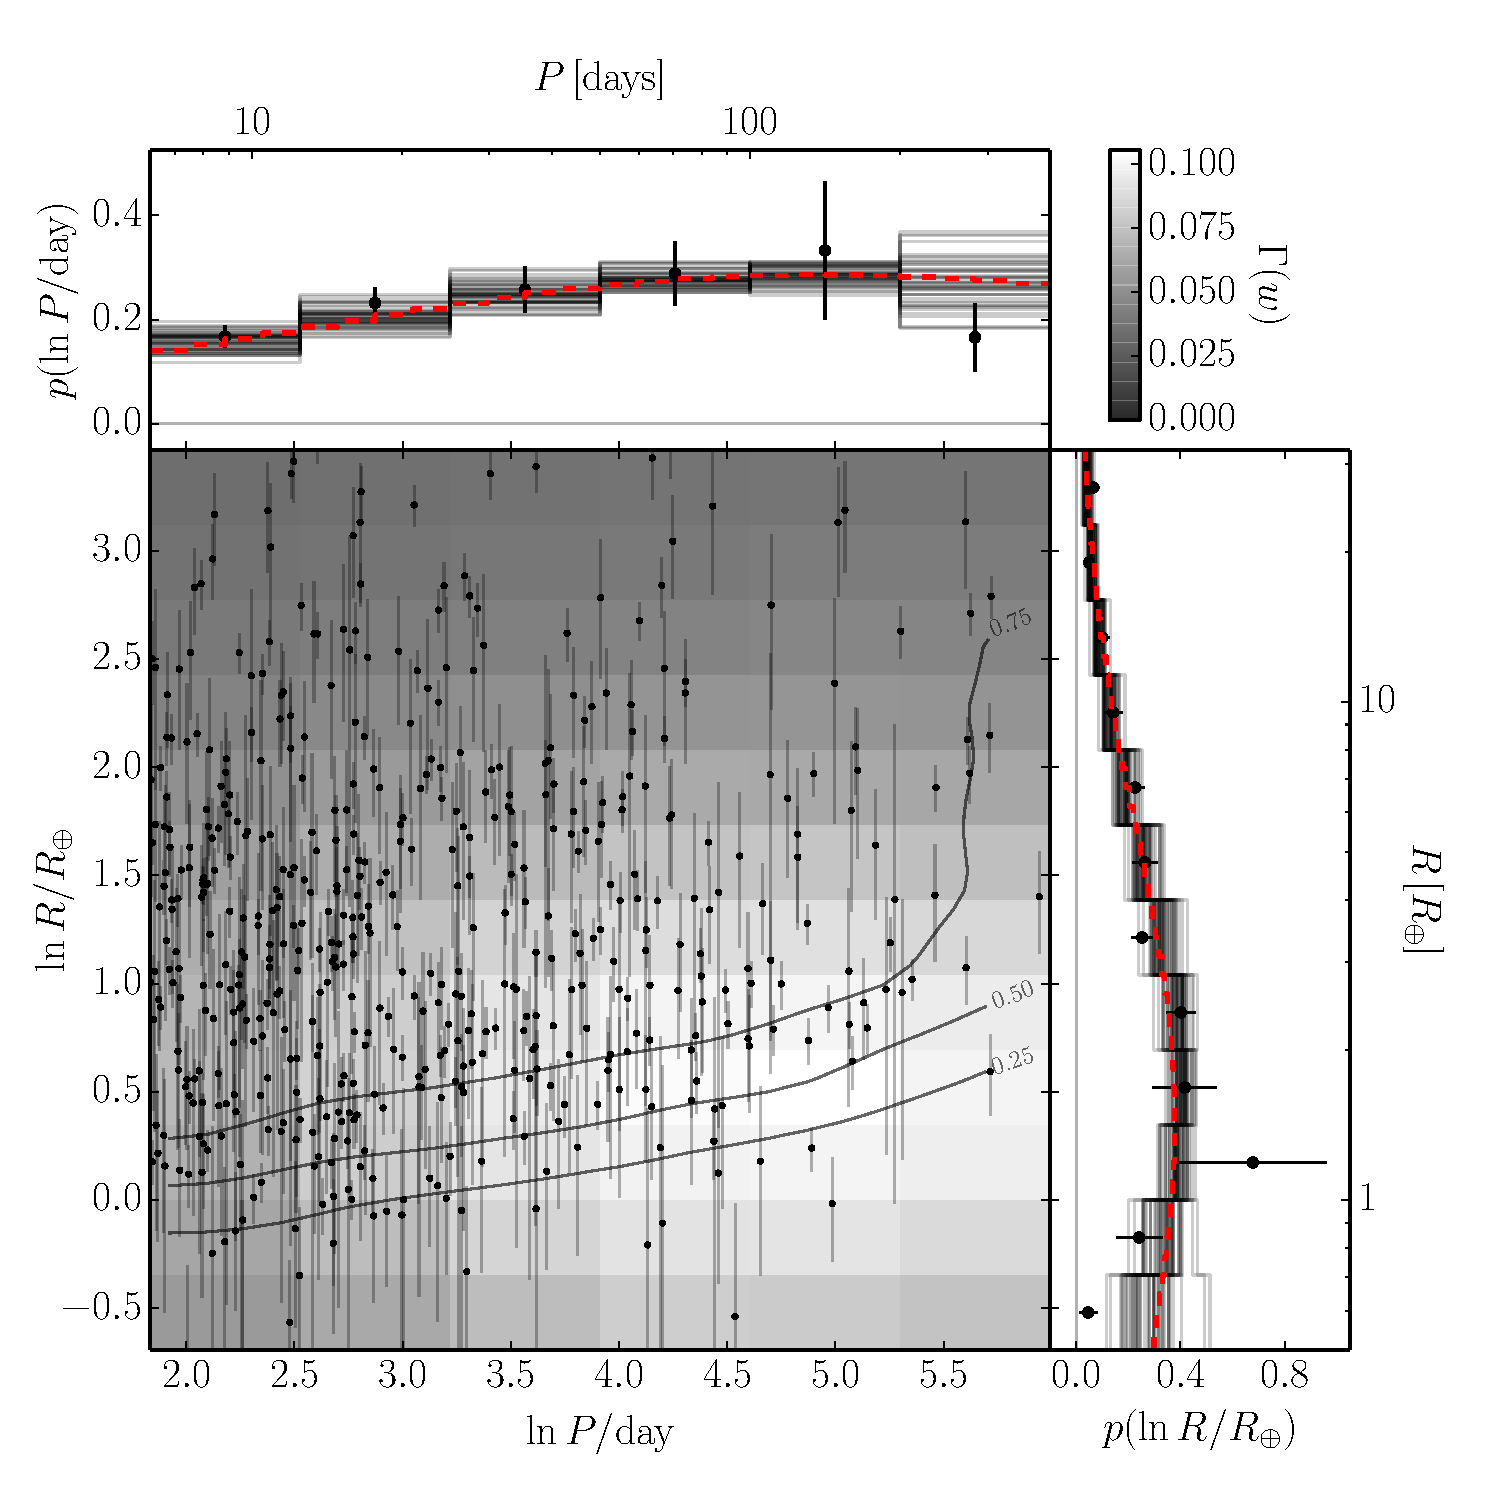
\includegraphics[width=\textwidth]{figures/exopop/smooth/results.pdf}
\end{center}
\caption[The inferred planet population for the simulated catalog \modela]{%
{\bf Simulated data}.
Inferences about the rate density based on the simulated catalog \modela.
\emph{Center:} the points with error bars show the exoplanet candidates in the
simulated incomplete catalog, the contours show the survey completeness
function (\citealt{Petigura:2013}), and the grayscale shows the median posterior
occurrence surface.
\emph{Top and left:} the red dashed line shows the true distribution that was
used to generate the catalog, the points with error bars show the results of
the inverse-detection-efficiency procedure, and the histograms are posterior
samples from the marginalized rate density as inferred by our method.
\figlabel{smooth-results}}
\end{figure}

\begin{figure}[p]
\begin{center}
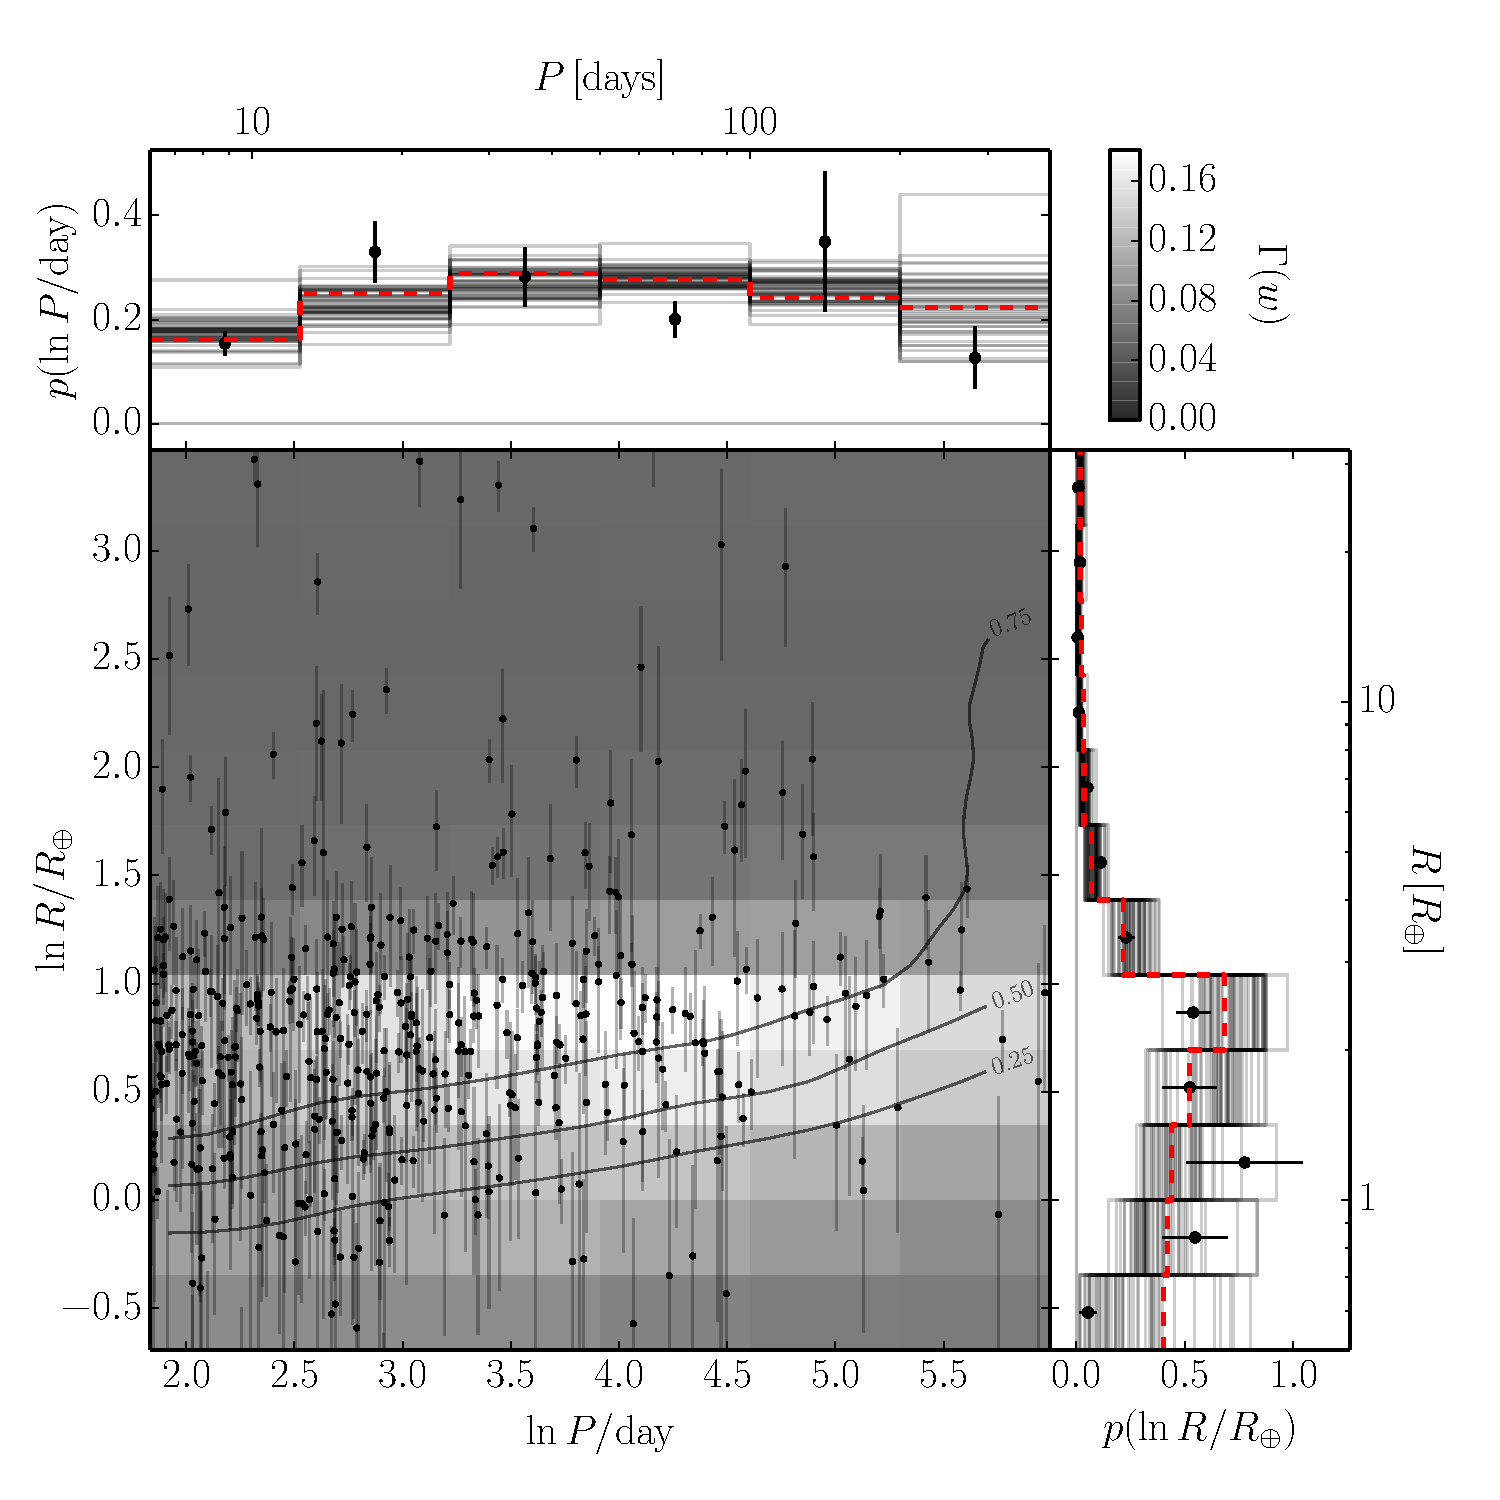
\includegraphics[width=\textwidth]{figures/exopop/simulation/results.pdf}
\end{center}
\caption[The inferred planet population for the simulated catalog \modelb]{%
{\bf Simulated data}.
The same as \fig{smooth-results} for \modelb.
\figlabel{simulation-results}}
\end{figure}

\section{Extrapolation to Earth}
\sectlabel{extrap}

As well as inferring the occurrence distribution of exoplanets, this dataset
can also be used to constrain the rate density of Earth analogs.
Explicitly, we constrain the occurrence rate density of exoplanets orbiting
``Sun-like'' stars\footnote{In this \paper, we adopt the \citet{Petigura:2013}
sample of G-stars as our definition of ``Sun-like''.}, evaluated at the
location of Earth:
\begin{eqnarray}\eqlabel{gammaearth}
\gammaearth &=& \rate (\ln\period_\oplus,\,\ln\radius_\oplus) \\
&=&
\left.\frac{\dd N}{\dd\ln\period\,\dd\ln\radius}\right|
_{\radius=\radius_\oplus,\,\period=\period_\oplus}\quad.
\end{eqnarray}
That is, \gammaearth\ is the rate density of exoplanets around a Sun-like
star (expected number of planets per star per natural logarithm of period per
natural logarithm of radius), evaluated at the period and radius of Earth.

In \eq{gammaearth}, we use the symbol $\Gamma$ instead of the more commonly
used $\eta$ since we define ``Earth analog'' in terms of measurable quantities
with no mention of habitability or composition.
This might seem unsatisfying but the composition of an exoplanet is
notoriously difficult to measure even with large uncertainty and any
definition of habitability is still extremely subjective.
With this in mind, we stick to the observable definition for this \paper.

Since no Earth analogs have been found, any constraints on this density must
be extrapolated from the existing observations.
This is generally done by assuming a functional form for the occurrence rate
density, constraining it using the observed candidates and extrapolating.
All published extrapolations are based on rigid models of the occurrence rate
density (for example, a power law) fit to the catalog and evaluated at the
location of Earth (\citealt{Catanzarite:2011, Traub:2012}).
\citet{Petigura:2013} used their catalog of planet candidates to constrain the rate
of Earth analogs in a specific period--radius bin assuming an extremely rigid
model: \emph{flat in logarithmic period}.
These results are all sensitive to the choice of extrapolation function and
the specific definition of ``Earth analog''.

We weaken the assumptions necessary for extrapolation by only assuming that
the distribution is smooth using the Gaussian process regularization described
in \sect{model}.
Under this model, the occurrence rate density at periods and radii where no
objects have been detected will be constrained---with large uncertainty---by
the heights of nearby bins.
Therefore, even though there are no candidates that qualify as Earth analogs,
we simply fit our model of the occurrence rate density in a large enough
region of parameter space (including Earth) and compute the posterior
constraints on \gammaearth.
This works because the Gaussian process regularization actually captures our
prior beliefs about the shape of the rate density function.
This model---and any other extrapolation---will, of course, break down if
there is an unmeasured sharp feature in the occurrence rate density near the
location of Earth but our method is the most conservative extrapolation
technique published to date.

For comparison, we also implemented and applied the extrapolation technique
applied by \citet{Petigura:2013}.
Their method assumes that, for small planets ($1 \le \radius/\radius_\oplus <
2$) on long periods ($\period > 50\,\mathrm{days}$), the occurrence rate
density is a flat function of logarithmic period or, equivalently, the
cumulative rate is linear.
\citet{Petigura:2013} used the candidates in their catalog to estimate the slope of
the empirical cumulative period distribution and used that function to
extrapolate.
Instead of defining \gammaearth\ differentially, as we did in \eq{gammaearth},
\citet{Petigura:2013} constrained the integral of the rate density over a box in
period and radius ($1 \le \radius/\radius_\oplus < 2$ and $200 \le
\period/\mathrm{day} < 400$).
Since their model implicitly assumes a constant rate density across the bin,
the differential rate is just their number divided by the bin volume.
This rate density (rate divided by bin volume) is what is shown as a
comparison to our results in the figures.

Figures~\figref{smooth-rate} and~\figref{simulation-rate} compare our results
and the results of the \citet{Petigura:2013} extrapolation procedure when applied
to the synthetic catalogs.
Since these catalogs were simulated from a known population model, we know the
true value of \gammaearth\ and it is indicated in the figures with a vertical
gray line.
In both cases, our method returns a less precise but more accurate result for
the rate density and the error bars given by the functional extrapolation
are overly optimistic.
One major effect that leads to this bias is that the period distribution is
not flat.
Restricting the result to only include uniform models is equivalent to
applying an extremely informative prior that doesn't have enough freedom to
capture the complexity of the problem.
As a result, the posterior constraints on \gammaearth\ are dominated by this
prior choice and the resulting uncertainties are much smaller than they should
be.

\begin{figure}[p]
\begin{center}
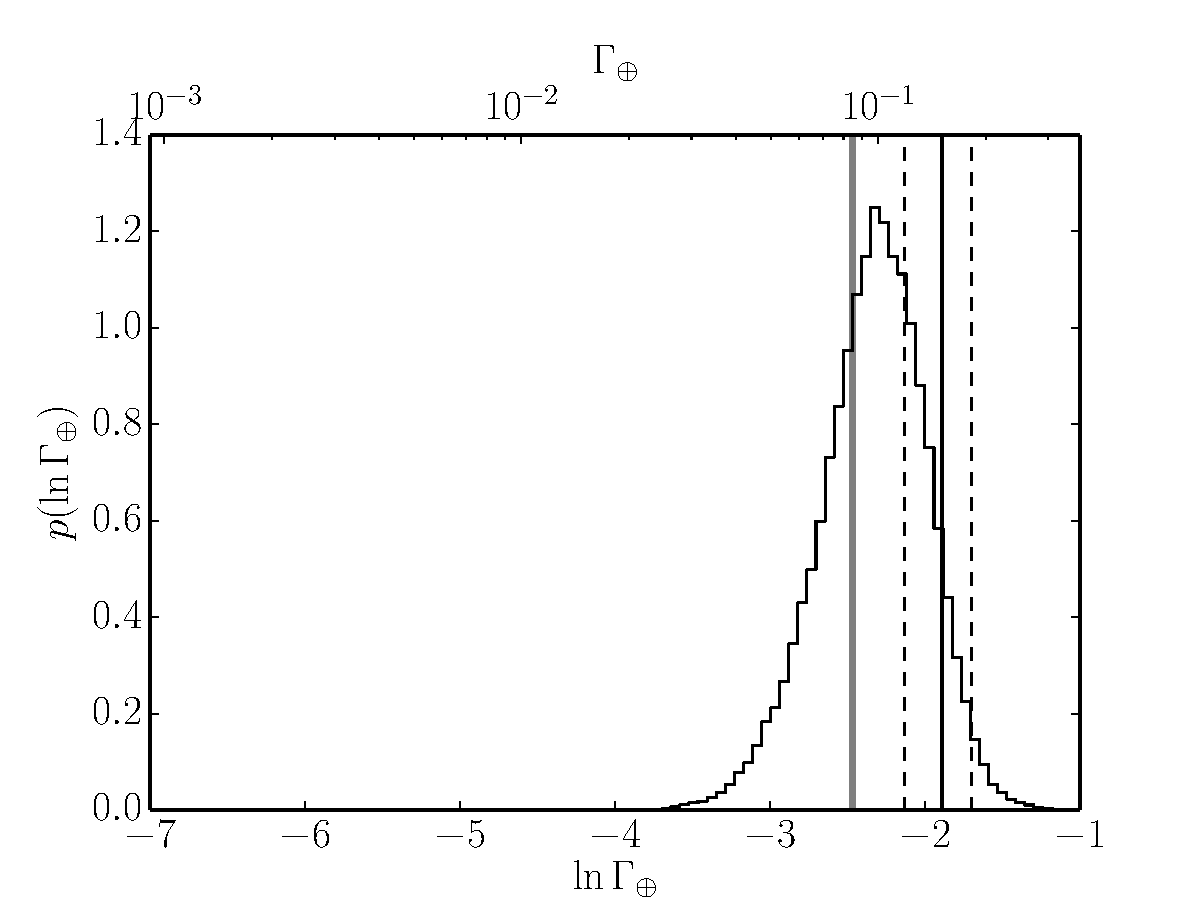
\includegraphics[width=0.8\textwidth]{figures/exopop/smooth/rate.pdf}
\end{center}
\caption[The inferred rate of Earth analogs for the simulated catalog \modela]{%
{\bf Simulated data}.
The extrapolated rate density of Earth analogs \gammaearth\ as inferred by the
different techniques applied to the \modela\ simulation.
Applying the method used by \citet{Petigura:2013} gives a constraint indicated by
the vertical black line with error bars shown as dashed lines.
The histogram is the MCMC estimate of our posterior constraint on this rate
density and the true value is indicated as the thick gray vertical line.
\figlabel{smooth-rate}}
\end{figure}

\begin{figure}[p]
\begin{center}
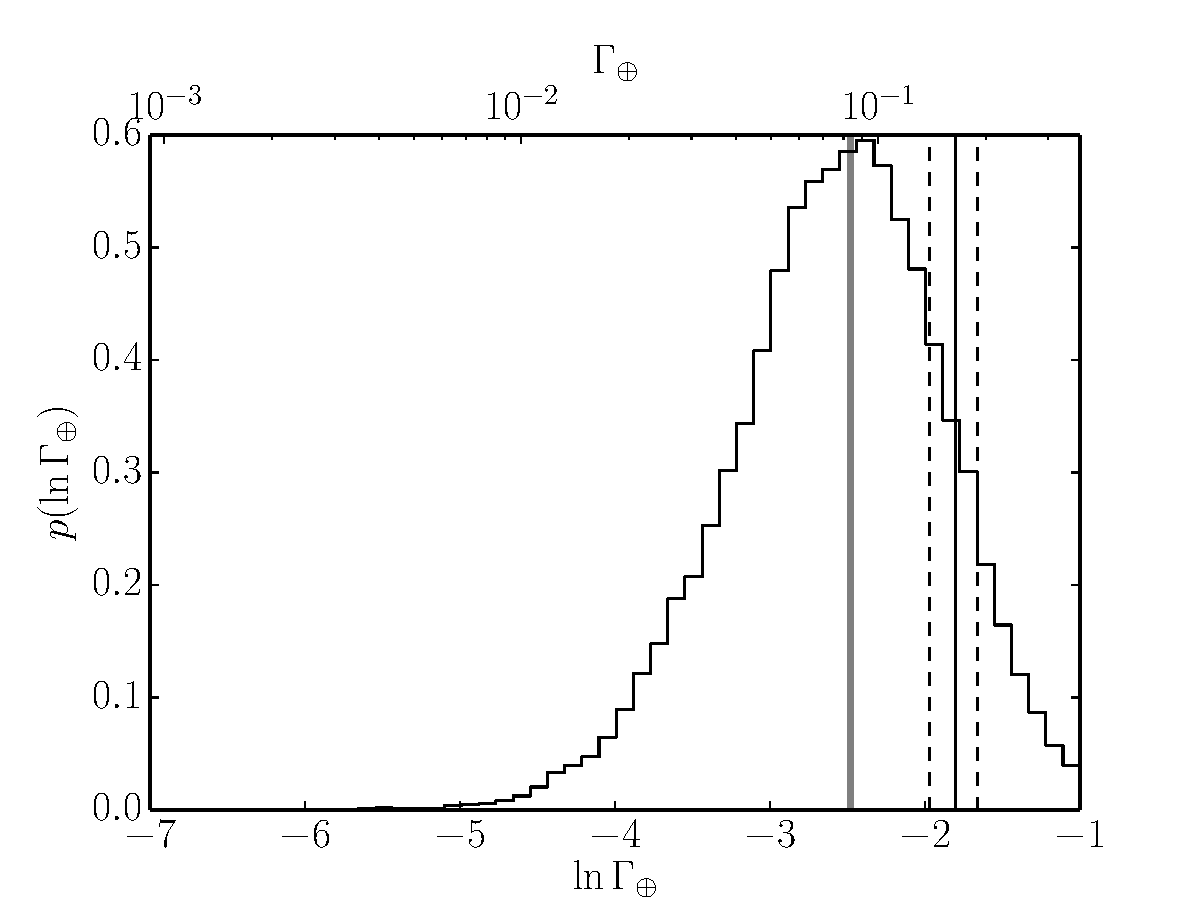
\includegraphics[width=0.8\textwidth]{figures/exopop/simulation/rate.pdf}
\end{center}
\caption[The inferred rate of Earth analogs for the simulated catalog \modelb]{%
{\bf Simulated data}.
The same as \fig{smooth-rate} for \modelb.
\figlabel{simulation-rate}}
\end{figure}

\section{Results from real data}
\sectlabel{real}

Having developed this probabilistic framework for exoplanet population
inferences and demonstrating that it produces reasonable results when applied
to simulated datasets, we now turn to real data.
As described in \sect{data}, we will use the catalog of small exoplanet
candidates orbiting Sun-like stars published by \citet{Petigura:2013}.
This is a great test case because those authors empirically measured the
detection efficiency of their pipeline as a function of the parameters of
interest.

We directly applied our method to the \citet{Petigura:2013} sample and generated
MCMC samples from the posterior probability for the occurrence rate density
step heights, marginalizing over the hyperparameters of the Gaussian process
model.
The resulting MCMC chain is available online\footnote{\resultsurl}.

\Fig{real-results} shows posterior samples from the inferred occurrence rate
density as a function of period and radius conditioned on the catalog.
The marginalized distributions are qualitatively consistent with the
occurrence rate density measured using the inverse-detection-efficiency
method with larger uncertainties.

The period distribution integrated over various radius ranges is shown in
\fig{period}.
In agreement with \citet{Dong:2013}, we find that the period distribution of large
planets ($R > 8\,R_\oplus$) is inconsistent with the distribution of smaller
planets.
The rate density of large planets appears to monotonically increase as a
function of log period while the distribution for small planets seems to turn
over at a relatively short period (around 50 days) and decrease for longer
periods.

The equivalent results for the radius distribution are shown in
Figures~\figref{radius} and~\figref{linear-radius}.
\Fig{radius} shows the log-radius occurrence rate density integrated over
various logarithmic bins in period.
The distributions in each period bin are qualitatively consistent; the
rate density is dominated by small planets (around two Earth radii) with
potential ``features'' near $\radius\sim3\radius_\oplus$ and $\radius\sim
10\radius_\oplus$.
These features appear in every period bin.
They were also detected---using a completely different dataset and
technique---by \citet{Dong:2013} and a similar result is visible in the occurrence
rate determined by \citet[][their Figure 7]{Fressin:2013} at low
signal-to-noise.
\Fig{linear-radius} shows the same result but presented as a function of
linear radius.
In these coordinates, the rate density in a single bin is no longer
uniform; instead, scales as inverse radius.

Our constraint on the rate density of Earth analogs (as defined in
\sect{extrap}) is in tension---even though our result has large fractional
uncertainty---with the result from \citet{Petigura:2013}.
This is shown in \fig{real-rate} where we compare the marginalized posterior
probability function for \gammaearth\ to the published value and uncertainty.
Quantitatively, we find that the rate density of Earth analogs is
\begin{eqnarray}\eqlabel{ge-result}
\gammaearth &=& 0.019^{+0.019}_{-0.010}~\densityunit
\end{eqnarray}
where the ``\densityunit'' indicates that this quantity is a rate density, per
natural logarithmic period per natural logarithmic radius.
Converted to these units, \citet{Petigura:2013} measured
$0.119_{-0.035}^{+0.046}~\densityunit$ for the same quantity (indicated as the
vertical lines in \fig{real-rate}).
This rate density is \emph{exactly} what Petigura's extrapolation model
predicts but, for comparison, we can also integrate our inferred rate density
over their choice of ``Earth-like'' bin ($200 \le \period/\mathrm{day} < 400$
and $1 \le \radius/\radius_\oplus < 2$) to find a \emph{rate} of
Earth analogs.
The published rate is $0.057_{-0.017}^{+0.022}$ (\citealt{Petigura:2013}) and our
posterior constraint is
\begin{eqnarray}
\int_{\period=200\,\mathrm{day}}^{400\,\mathrm{day}}
\int_{\radius=1\,\radius_\oplus}^{2\,\radius_\oplus}
\rate_\ratepars (\ln\period,\,\ln\radius)
\dd[\ln\radius]
\dd[\ln\period]
&=&
0.019_{-0.008}^{+0.010}
\quad.
\end{eqnarray}

Although they are mainly nuisance parameters, we also obtain posterior
constraints on the hyperparameters \mean\ and \smoothpars.
In particular, the constraints on the length scales in $\ln \period$ and $\ln
\radius$ are $\smooth_\period = 3.65 \pm 1.03$ and $\smooth_\radius = 0.65 \pm
0.12$ respectively.
Both of these scales are larger than a bin in their respective dimension.
For completeness we also find the following constraints on the other
hyperparameters
\begin{eqnarray}
\mean = 5.44 \pm 1.56 &\quad\mathrm{and}\quad&
\ln\smooth_0 = 1.68 \pm 0.72 \quad.
\end{eqnarray}
The MCMC chains used to compute these values is available
online\footnote{\resultsurl}.

\begin{figure}[p]
\begin{center}
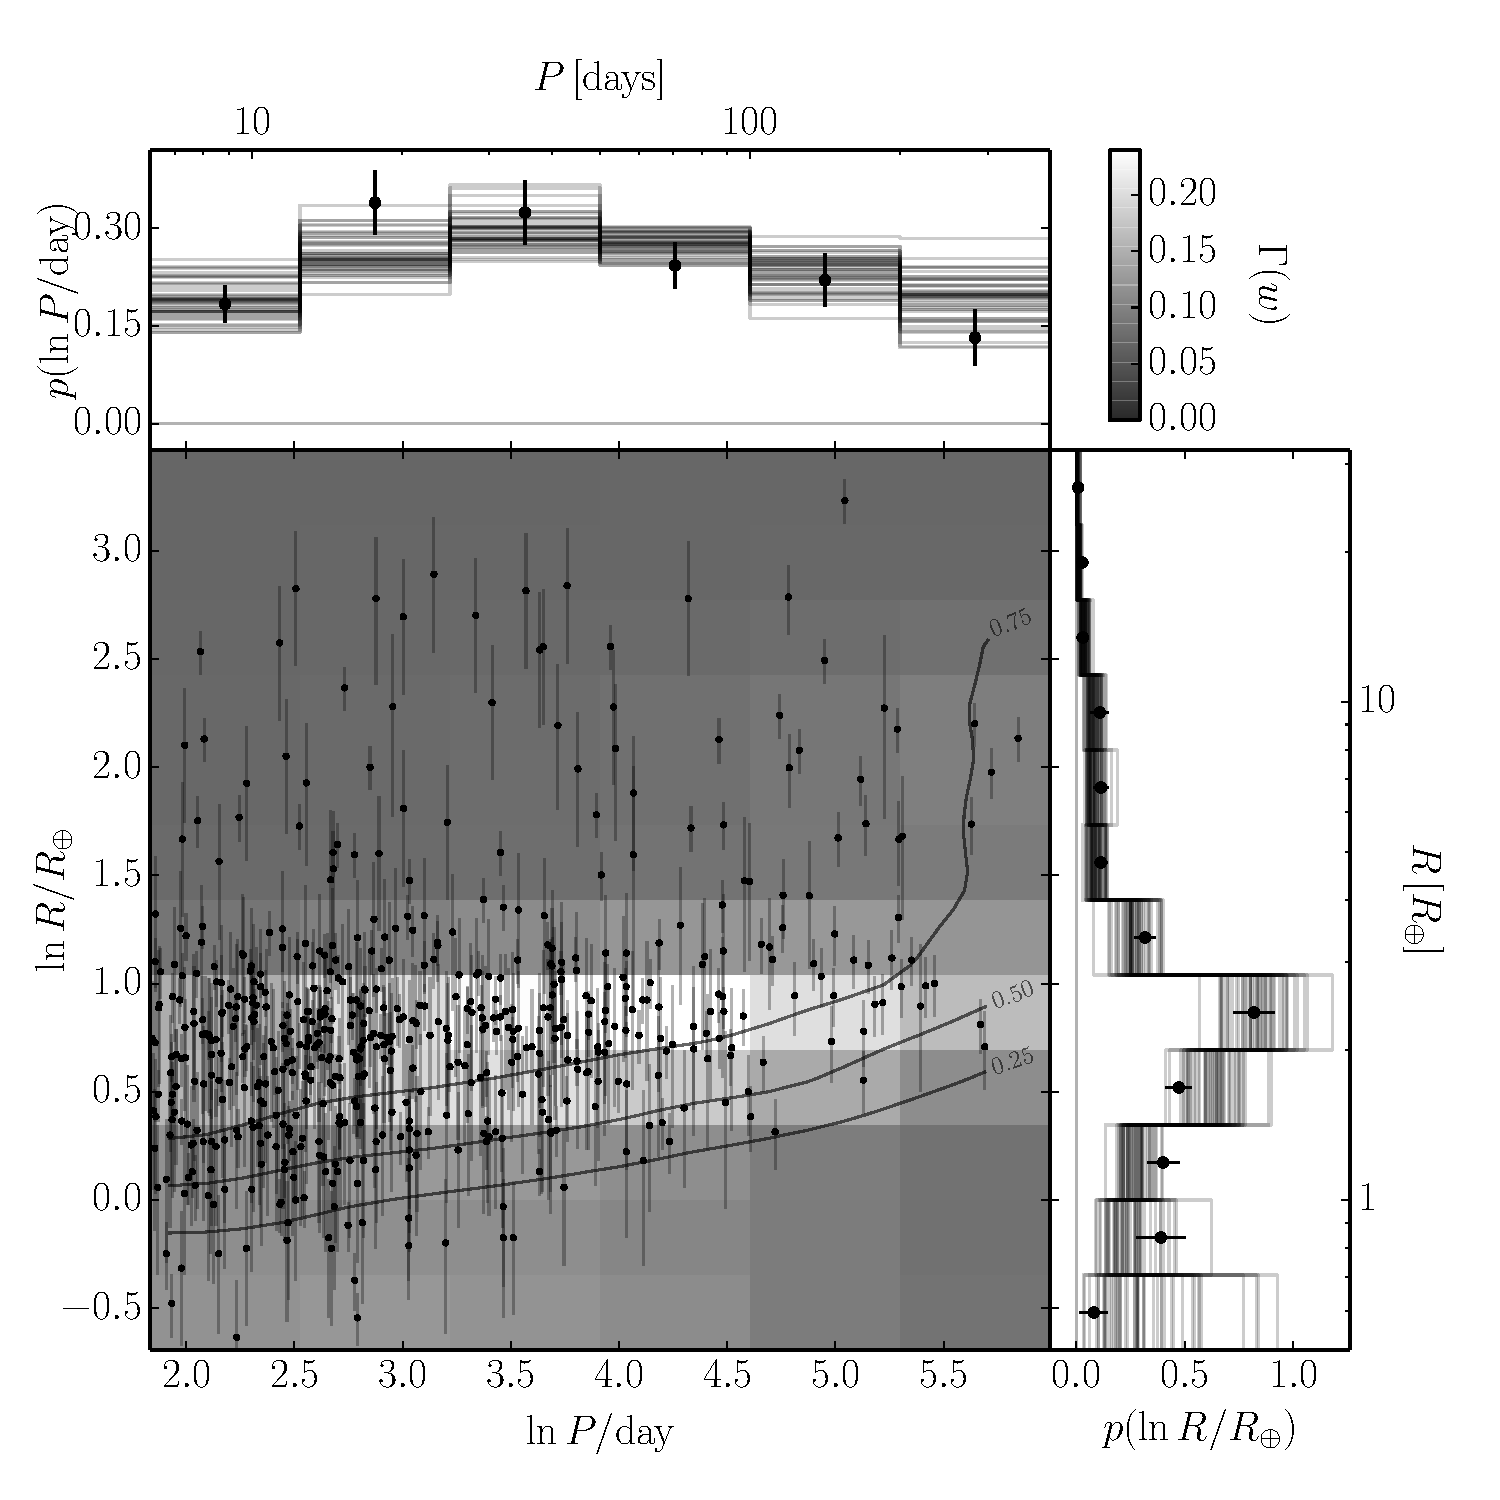
\includegraphics[width=\textwidth]{figures/exopop/results/results.pdf}
\end{center}
\caption[The population of exoplanets]{%
{\bf Real data}.
The same as \fig{smooth-results} when applied to the observed data from
\citet{Petigura:2013}.
\emph{Center:} the points with error bars show the catalog measurements, the
contours show the survey completeness function, and the grayscale shows the
median posterior occurrence surface.
\emph{Top and left:} the points with error bars show the results of the
inverse-detection-efficiency procedure, and the histograms are posterior
samples from the marginalized rate density as inferred by our method.
\figlabel{real-results}}
\end{figure}

\begin{figure}[p]
\begin{center}
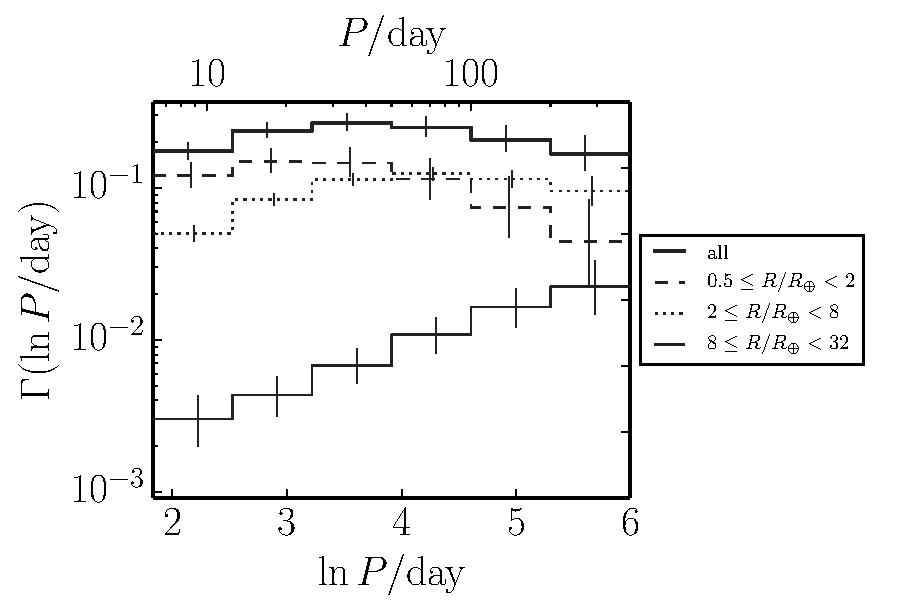
\includegraphics{figures/exopop/results/period.pdf}
\end{center}
\caption[The period distribution of exoplanets]{%
{\bf Real data}.
The occurrence rate density as a function of logarithmic period integrated
over bins in logarithmic radius.
The lines with error bars show the posterior sample median and 68th
percentile and the line style specifies the radius bin.
The period distribution for the largest planets in the sample
($8 \le R/R_\oplus < 32$) continues to increase (as a function of
$\ln\period$) for all periods while the distribution seems to flatten and
turn over at periods around 50 days.
\figlabel{period}}
\end{figure}

\begin{figure}[p]
\begin{center}
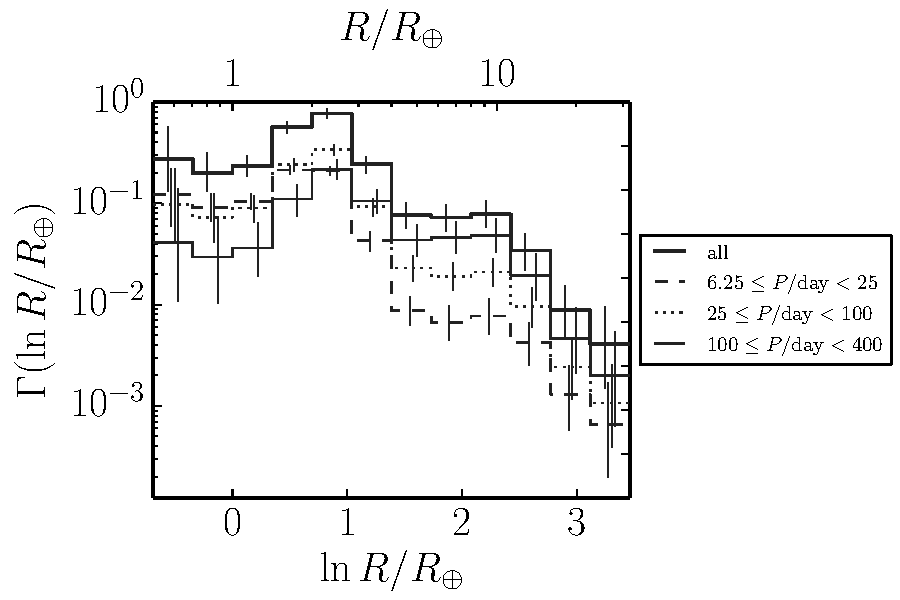
\includegraphics{figures/exopop/results/radius.pdf}
\end{center}
\caption[The radius distribution of exoplanets]{%
{\bf Real data}.
The occurrence rate density as a function of logarithmic radius integrated
over bins in logarithmic period.
The lines with error bars show the posterior sample median and 68th
percentile and the line style specifies the period bin.
The distributions in all the period bins are qualitatively consistent and
there are plausibly features near $R\sim3\,R_\oplus$ and $R\sim10\,R_\oplus$.
\figlabel{radius}}
\end{figure}

\begin{figure}[p]
\begin{center}
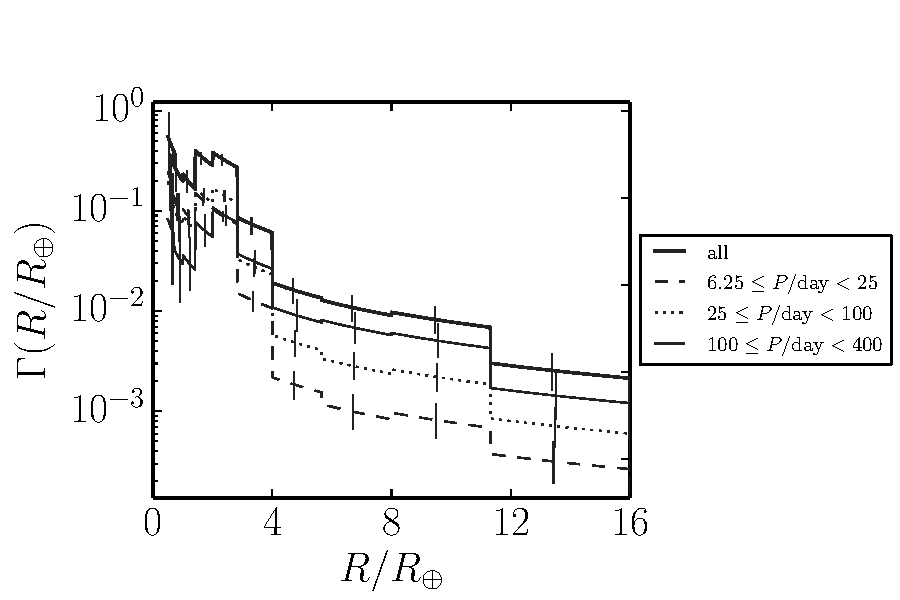
\includegraphics{figures/exopop/results/linear-radius.pdf}
\end{center}
\caption[The radius distribution of exoplanets plotted in terms of linear
radius]{%
{\bf Real data}.
The same as \fig{radius} but presented as a density in radius instead of
logarithmic radius.
\figlabel{linear-radius}}
\end{figure}

\begin{figure}[p]
\begin{center}
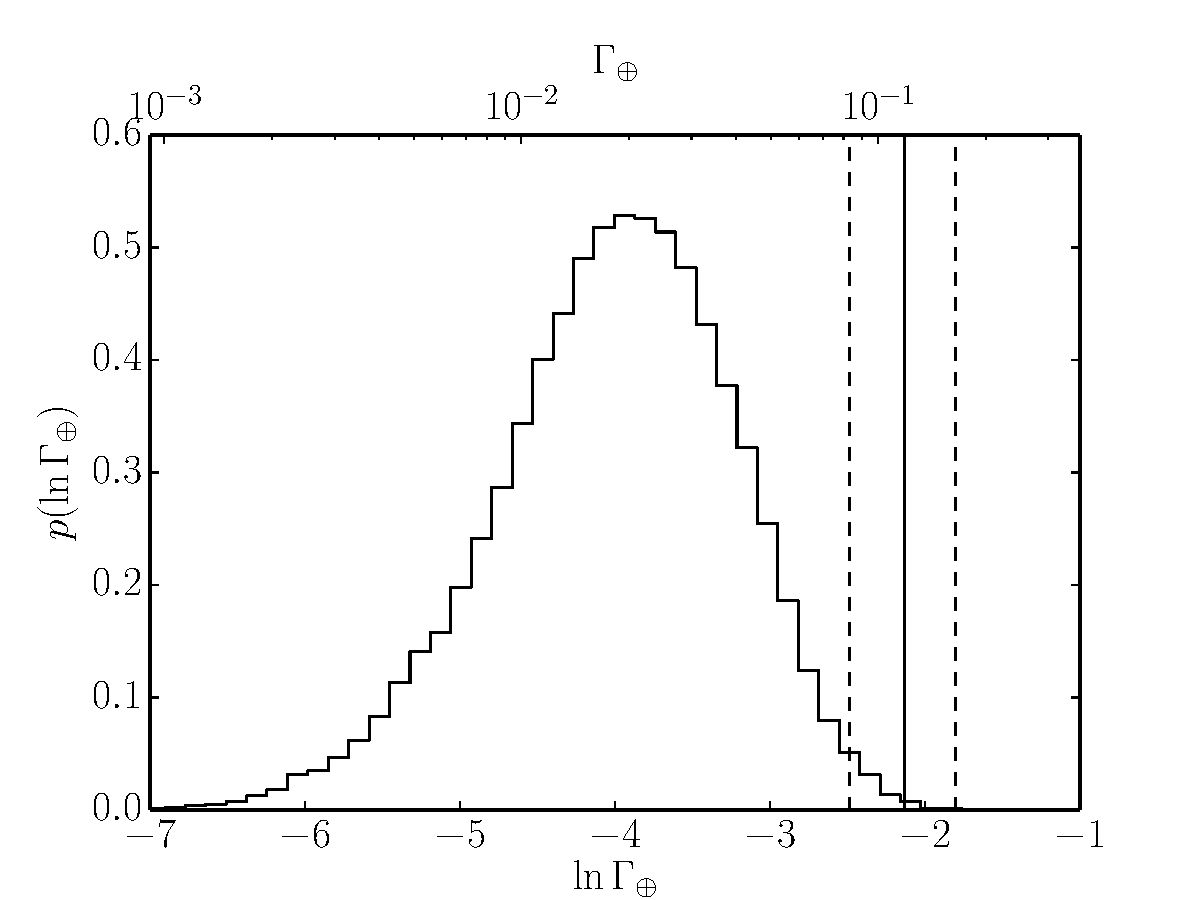
\includegraphics[width=0.8\textwidth]{figures/exopop/results/rate.pdf}
\end{center}
\caption[The rate of Earth analogs]{%
The extrapolated rate density of Earth analogs \gammaearth\ (the same as
\fig{smooth-rate} but applied to the catalog from \citealt{Petigura:2013}).
The histogram is the MCMC estimate of our posterior constraint on this rate
density.
The vertical black line with error bars shown as dashed lines is the result
from \citet{Petigura:2013} converted to a rate density by dividing by their bin
volume.
\figlabel{real-rate}}
\end{figure}

\section{Comparison with previous work}
\sectlabel{comparison}

Our inferred rate density of Earth analogs (\eqalt{ge-result}) is not
consistent with previously published results.
In particular, our result is completely inconsistent with the earlier result
based on \emph{exactly the same dataset} (\citealt{Petigura:2013}).
This inconsistency is due to the different assumptions made and the detailed
cause merits some investigation.
The two key differences between our analysis and previous work are \emph{(a)}
the form of the extrapolation function, and \emph{(b)} the presence of
measurement uncertainties on the planet radii.

To make their estimate of \gammaearth, \citet{Petigura:2013} asserted a flat
distribution in logarithmic period for small planets.
Our results suggest that the data \emph{do not support} this assumption (see
\fig{period}).
We find that the data require a \emph{decreasing} period distribution in the
relevant range.
A similar result was also found by \citet{Dong:2013} and it is apparent in Figure 2
of \citet{Petigura:2013}.

To test the significance of the choice of extrapolation function, we relax the
assumption of a uniform period distribution and allow the distribution to be
linear in the same range ($R=1-2\,R_\oplus$ and $P=50-400\mathrm{d}$).
Under this model, the likelihood of the catalog of planets in this range can
be calculated using \eq{poisson-like}.
We apply uniform priors in the physically allowed range of slopes and
intercepts for this distribution and estimate the posterior probability for
the extrapolated rate using MCMC (\citealt{Foreman-Mackey:2013}).
This results give a much more uncertain and substantially lower estimate for
the rate of Earth analogs
\begin{eqnarray}
\Gamma_\oplus &=& 0.072^{+0.088}_{-0.047} \quad.
\end{eqnarray}
With the large error bars, this result is consistent with both results (see
\fig{comparison} where this value is labeled ``linear extrapolation'') but it
does not fully account for the discrepancy.

To examine the effects of measurement uncertainties, we repeat our analysis
with the error bars on the radii artificially set to zero, keeping everything
else the same.
This analysis (labeled ``uncertainties ignored'' in \fig{comparison}) gives
the result
\begin{eqnarray}
\Gamma_\oplus &=& 0.040^{+0.031}_{-0.019} \quad.
\end{eqnarray}
This result is relatively more precise and higher than our final result and
consistent with the value obtained with linear extrapolation.
This confirms the hypothesis that the discrepancy between our result and the
previously published values is the combined result of both of our key
generalizations.

For comparison, we have also included the value of \gammaearth\ implied by
\citet[][their Table 2]{Dong:2013}.
This result is based on a power law fit to the period distribution of small
planets ($R=1-2\,R_\oplus$) on long periods ($P=10-250\,\mathrm{d}$) in a
different catalog (\citealt{Batalha:2013}) with a parametric completeness
model.
There are a few factors to consider when comparing to this to our analysis.
Firstly, while \citet{Dong:2013} fit a power law in log period, this is still a
very restrictive model when considering this large range of periods.
A broken power law might be more applicable.
Furthermore, their analysis did not incorporate the effects of measurement
uncertainties.
Finally, unlike the \citet{Petigura:2013}, the \citet{Batalha:2013} catalog used
by \citet{Dong:2013} includes multiple transiting systems.
As mentioned previously, the effect of this selection is hard to determine
without further investigation but it should, intuitively, cause any inference
based on the \citet{Petigura:2013} sample to be an underestimate of the \True\
rate.

\begin{figure}[p]
\begin{center}
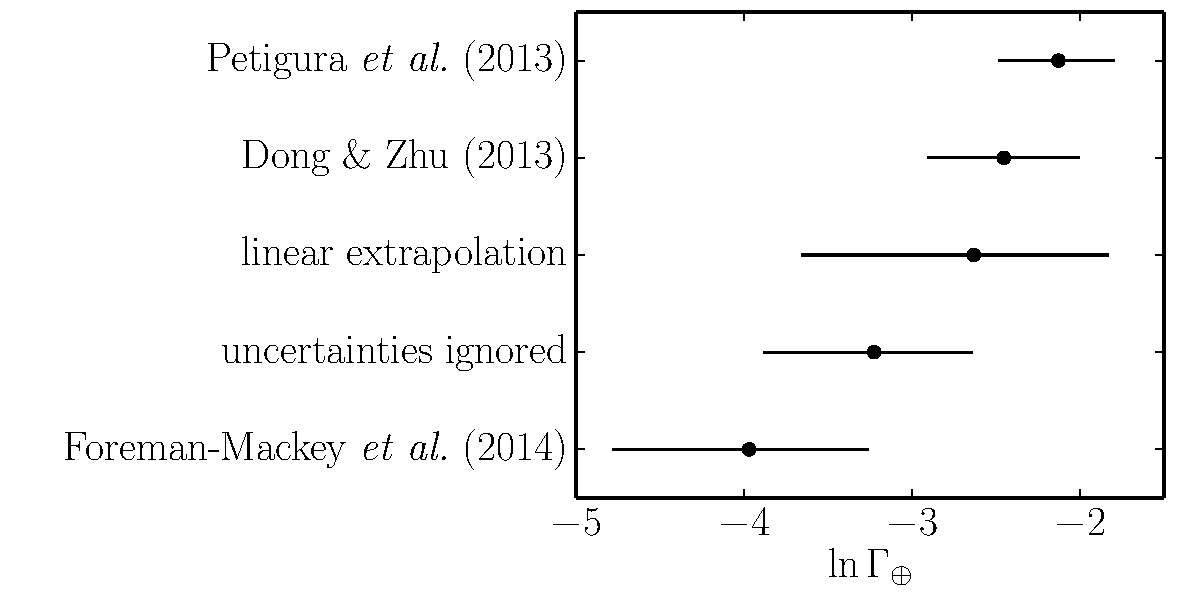
\includegraphics[width=\textwidth]{figures/exopop/comparison.pdf}
\end{center}
\caption[Comparison to literature values for the rate of Earth analogs]{%
Comparison of various estimates of \gammaearth.
From the top, the first value is the number published by \citet{Petigura:2013} and
converted to consistent units.
The second point shows the value implied by the power law model for the
occurrence rate of $1-2\,R_\oplus$ planets from \citet{Dong:2013}.
The point labeled ``linear extrapolation'' is the result of modeling the
distribution of small planets ($1-2\,R_\oplus$) on long periods
($50-400\,\mathrm{days}$) but allowing the period distribution to be
\emph{linear} instead of \emph{uniform}.
The ``uncertainties ignored'' value is given by applying the model
developed in this \paper\ but with the error bars on radius artificially
set to zero.
Finally, the bottom point is the result of our full analysis.
\figlabel{comparison}}
\end{figure}

\section{Discussion}

We have developed a hierarchical probabilistic framework for inferring the
population of exoplanets based on noisy incomplete catalogs.
This method incorporates systematic treatment of observational uncertainties
and detection efficiency.
One major benefit of this framework is that it provides the best possible
probabilistic measurements of the population under the assumptions listed in
\sect{intro} and repeated below.
After demonstrating the validity of our method on two qualitatively different
synthetic exoplanet catalogs, we run our inference on a published catalog of
small exoplanet candidates orbiting Sun-like stars (\citealt{Petigura:2013}) to
determine the occurrence rate density these planets as a function of period
and radius.
We extrapolate this measurement to the location of Earth and constrain the
rate density of Earth analogs with large error bars.
In order to perform this extrapolation, we don't assume a specific functional
form for the rate density.
Instead, we only assume that it is a smooth function of logarithmic period and
radius.

The occurrence rate density function that we infer is qualitatively consistent
with previously published results using different inference techniques
(\citealt{Dong:2013, Fressin:2013, Petigura:2013}).
In particular, we find (see \fig{radius}) previously recorded features in the
radius distribution around $\radius\sim 3\,\radius_\oplus$ and $\radius\sim
10\,\radius_\oplus$, although not at high signal-to-noise.
We find that the period distributions for planets in different radius bins are
different, in qualitative agreement with previous results (\citealt{Dong:2013}).
\Fig{period} shows that larger planets tend to be on longer periods than
smaller planets.

% In detail, any inference of the exoplanet population depends on the choices
% made in the pipeline that creates the catalog.
% Our results are based on a catalog that only includes single transiting
% systems (\citealt{Petigura:2013}) so our conclusions---and theirs---must be
% considered with this in mind.
% In particular, the exclusion of second (and third, and so on) planets must
% suppress the inferred rate density, especially at long periods and small
% radii.

Our extrapolation of the rate density to the location of Earth is more general
and conservative than any previously published method.
We find a rate density of Earth analogs that is inconsistent with the result
published by \citet{Petigura:2013}.
This discrepancy can be attributed to both the rigidity of the assumptions
about the period distribution and the effects of non-negligible measurement
uncertainties.
Our extrapolation is also less confident than previous measurements.
Again, this difference is due to the fact that we allow a much more flexible
extrapolation function.
This is another illustration that, against the standard data analysis
folklore, the correct use of flexible models is \emph{conservative}.

In contrast to previous work, we don't define ``Earth analog'' in terms of
habitability or composition.
Instead, we advocate for a definition in terms of more directly observable
quantities (in this case, period and radius).
Furthermore, we define \gammaearth\ as a rate density (per star per
logarithmic period per logarithmic radius) so that its value doesn't depend on
choices about the ``Earth-like'' bin.

In our analysis we make a few simplifying assumptions.
Every assumption has an effect on the results and could be relaxed as an
extension of this project.
For completeness, we list and discuss the effects of our assumptions below.
\begin{itemize}

\item {\bf Conditional independence}\quad
We assume that every object in the catalog is a conditionally independent
draw from the observable occurrence rate density.
This is a bad assumption when applying this method to a different catalog
where multiple transiting systems are included.
In practice, the best first step towards relaxing this assumption is probably
to follow \citet{Tremaine:2012} and assume that the mutual inclination
distribution is the only source of conditional dependence between planets.
For this \paper, the assumption of conditional independence is justified
because the dataset explicitly includes only systems with a single transiting
exoplanet.

\item {\bf False positives}\quad
In our inferences, we assume that all of the candidates in the catalog are
\True\ exoplanets.
The rate of false positives in the \kepler\ catalog has been shown to be low
but not negligible (\citealt{Morton:2012, Fressin:2013}).
Since some of the objects in the catalog are probably false positives, our
inferences about the occurrence rate density are biased high but without
explicitly including a model of false positives, it's hard to say in detail
what effect this would have on the distributions.
In an extension of this work, we could incorporate the effects of false
positives by switching to a mixture model (see \citealt{Hogg:2010}, for
example) where each object is modeled as a mixture of \True\ exoplanet and
false positive.
In this mixture model, the false positives would be represented using prior
distributions similar to those used by \citet{Morton:2012} or
\citet{Fressin:2013}.

\item {\bf Known observational uncertainties}\quad
To apply the importance sampling approximation to the published catalog, we
assume that the measurement uncertainties are known and, in this case,
Gaussian.
The assumption of normally distributed uncertainties could be relaxed given
a sampling representation of the posterior probability function for the
physical parameters (period, radius, \etc).
There is recent evidence that the stellar radii of \kepler\ targets might, on
average, be underestimated (\citealt{Bastien:2014}), introducing another
source of noise.
It is possible to relax the noise model and include effects like this but
inference would be substantially more computationally expensive.

\item {\bf Given empirical detection efficiency}\quad
\citet{Petigura:2013} determined the end-to-end detection efficiency of their
planet detection pipeline as a function of \True\ period and radius by
injecting synthetic signals into real light curves and testing recovery.
We used these simulations as an exact representation of the detection
efficiency of the catalog but there are several missing components.
The biggest effect is probably the fact that this formulation doesn't include
the selection of only the \emph{most detectable signal} in each light curve.
This bias will be largest in the parts of parameter space where the baseline
detection efficiency is lowest: at long periods and small radius.
As a result, our inferences (and the results from \citealt{Petigura:2013}) about
the occurrence rate of small planets on long periods is probably
\emph{underestimated} relative to \Truth.
In detail there is another limitation due to the fact that the stellar
parameters are only known noisily and the transit light curve only constrains
the radius ratio.
This means that the marginalized detection efficiency should be measured as a
function of radius ratio and the interpretation in terms of \True\ radius is
only approximately correct.
Given the size of the dataset and the number of injection simulations, this
effect should be small.

\item {\bf Smooth rate function}\quad
Throughout our analysis, we make the prior assumption that the occurrence rate
density is a smooth function of logarithmic period and radius.
This model is useful because it allows us to make probabilistically justified
inferences about the exoplanet population in regions of parameter space with
low detection efficiency.
The assumption that the rate density should be smooth is intuitive but there
is no theoretical indication that it must be true at all scales.
That being said, the Gaussian process regularization that we use to enforce
smoothness is flexible enough to capture substantial departures from smooth if
they were supported by the data.

\end{itemize}
Our assumptions are severe but we believe that this is the most conservative
population inference method currently on the market.

Under the assumptions that we have made here, our inference of the occurrence
rate density of exoplanets places a probabilistic constraint on the number of
transiting Earth analogs in the existing \kepler\ dataset.
If we adopt the definition of ``Earth-like'' from \citet[][$200 \le
\period/\mathrm{day} < 400$ and $1 \le \radius/\radius_\oplus <
2$]{Petigura:2013},
and integrate the product inferred rate density function and the geometric
transit probability (\eqalt{transitprob}) over this bin, we find that the
expected number of Earth-like exoplanets transiting the stars in the sample of
Sun-like stars chosen by \citet{Petigura:2013} is
\begin{eqnarray}\eqlabel{ntransit}
N_{\oplus,\,\mathrm{transiting}} &=& 10.6_{-4.5}^{+5.9}
\end{eqnarray}
where the uncertainties are only on the expectation value and don't include
the Poisson sampling variance.
This is an exciting result because it means that, if we can improve the
sensitivity of exoplanet search pipelines to small planets orbiting on long
periods, then we should find some Earth analogs in the existing data.
Furthermore, because of the treatment of multiple transiting systems in the
catalog, the \True\ expected number of transiting Earth-like exoplanets
orbiting Sun-like stars is almost certainly larger than the values in
\eq{ntransit}!

Some of the caveats on the results in this paper are due to assumptions made
for computational simplicity but a much more robust study would be possible
given a complete representation of the posterior probability function for the
physical parameters in the catalog.
The use of MCMC to fit models to observations is becoming standard practice in
astronomy and the results in many catalogs (including \citealt{Petigura:2013}) are
given as statistics computed on posterior samplings.
For the sake of hierarchical inferences like the method presented here, it
would be very useful if the authors of upcoming catalogs also published
samples from these distributions \emph{along with the value of their prior
function evaluated at each sample}.
In this spirit, we have released the results of this paper as posterior
samplings\footnote{\resultsurl} for the occurrence rate density function.

All of the code used in this project is available from
\url{http://github.com/dfm/exopop} under the MIT open-source software license.
This code (plus some dependencies) can be run to re-generate all of the
figures and results in this \paper.

\section{Appendix: Inverse-detection-efficiency}
\sectlabel{inv-det-eff}

One huge benefit of the inverse-detection-efficiency procedure is its
simplicity.
Therefore, it's worth noting that there is a probabilistically justified
procedure that will always provide less biased results while being only
marginally more complicated.

The standard procedure involves making a weighted histogram of the catalog
entries where the weight for object $\entry_k$ is $1/\completeness(\entry_k)$.
This makes intuitive sense but it does not have a clear probabilistic
justification or interpretation.
As we will show below, the maximum likelihood result involves weighting the
points by the inverse of the \emph{integral} of the completeness function over
the bin area.

To motivate this derivation, let's start by considering the following
pathological example: a single bin where the completeness sharply drops from
one to zero halfway across the bin.
If we observe $K$ objects in this bin, we would have observed about $2K$
objects in a complete sample.
If we apply the inverse-detection-efficiency procedure to this dataset, each
sample will get unit weight because they are all found in the part of the bin
where the completeness is one.
Therefore, we would \emph{underestimate} the true rate in the bin by half.
It's clear in this specific case that giving the points a weight of two would
give a better solution and we'll derive the general result below.

If we model the occurrence rate density as a histogram with $J$ fixed bin
volumes $\binarea_j$ (\eqalt{rate-model}) then \eq{poisson-like} becomes
\begin{eqnarray}
\ln p(\{\entry_k\}\,|\,\ratepars) &=&
    \sum_{k=1}^K \sum_{j=1}^J \mathbf{1}[\entry_k \in
        \binarea_j]\,[\ln\completeness(\entry_k)+\ratepar_j]
    -\sum_{j=1}^J\exp(\ratepar_j)\,
        \int_{\binarea_j} \completeness(\entry)\dd\entry
\end{eqnarray}
where the indicator function $\mathbf{1}[\cdot]$ is one if $\cdot$ is true and
zero otherwise.
Taking the gradient of this function with respect to \ratepars\ and setting it
equal to zero, we find the maximum likelihood result
\begin{eqnarray}\eqlabel{ml-ide}
\exp ({\ratepar_j}^*) &=&
\frac{K_j}{\int_{\binarea_j} \completeness(\entry)\dd\entry}
\end{eqnarray}
where $K_j$ is the number of objects that fall within the bin $j$.
We estimate the uncertainty $\delta\ratepar_j$ on this value by examining the
curvature of the log-likelihood function near the maximum and find
\begin{eqnarray}
\frac{\delta\exp({\ratepar_j}^*)}{\exp({\ratepar_j}^*)}
&=& \frac{1}{\sqrt{K_j}}
\quad.
\end{eqnarray}

In our pathological example from above, the integral of the completeness
function over the bin is $1/2$, giving each sample the expected weight of $2$.
In more realistic cases, where the completeness function varies smoothly, the
inverse-detection-efficiency result will begin to agree with \eq{ml-ide} but
the severity of this bias will be very problem dependent.
Therefore, if you have a dataset with negligible observational uncertainties,
we recommend that you always apply \eq{ml-ide} instead of the standard
inverse-detection-efficiency procedure.
As the uncertainties become more significant, there is no longer an analytic
result and the method derived in this \paper\ is necessary.

\section{Chapter Acknowledgements}

We would like to thank Erik Petigura (Berkeley) for freely sharing his data
and code.
It is a pleasure to thank
Ruth Angus (Oxford),
Tom Barclay (NASA Ames),
Jo Bovy (IAS),
Eric Ford (PSU),
David Kipping (CfA),
Ben Montet (Caltech/Harvard), and
Scott Tremaine (IAS)
for helpful contributions to the ideas and code presented here.
We would also like to acknowledge the anonymous referee and the Scientific
Editor, Eric Feigelson, for suggestions that
substantially improved the paper.
This research made use of the NASA \project{Astrophysics Data System}.

\renewcommand{\chapid}{ketu}

\renewcommand{\kepler}{\project{Kepler}}
\newcommand{\KT}{\project{K2}}
\newcommand{\tess}{\project{TESS}}
\newcommand{\jwst}{\project{JWST}}
\newcommand{\pdc}{\project{PDC}}

\newcommand{\BIC}{{\ensuremath{\mathrm{BIC}}}}
\newcommand{\T}{\ensuremath{\mathrm{T}}}

\newcommand{\flux}{{\ensuremath{f}}}
\newcommand{\ferr}{{\ensuremath{\sigma_\flux}}}
\newcommand{\attime}{{\ensuremath{t}}}
\newcommand{\basis}{{\bvec{A}}}
\newcommand{\weights}{{\bvec{w}}}

\renewcommand{\period}{{\ensuremath{P}}}
\newcommand{\phase}{{\ensuremath{T^0}}}
\newcommand{\duration}{{\ensuremath{D}}}
\newcommand{\depth}{{\ensuremath{Z}}}
\newcommand{\transittime}{{\ensuremath{T}}}
\newcommand{\impact}{{\ensuremath{b}}}
\newcommand{\ecc}{{\ensuremath{e}}}
\newcommand{\pomega}{{\ensuremath{\omega}}}

\newcommand{\datareleaseurl}{{\url{http://bbq.dfm.io/ketu}}}

\newcommand{\response}[1]{#1}

\chapter{A systematic search for transiting planets in the \KT\ data}

This \paper\ is joint work with Benjamin~T.~Montet (Caltech, Harvard),
David~W.~Hogg (NYU), Timothy~D.~Morton (Princeton), Dun~Wang (NYU), and
Bernhard~Sch\"olkopf (MPIS) submitted to \emph{The Astrophysical Journal} as
Foreman-Mackey et al.\ (2015).

\section{Chapter Abstract}

Photometry of stars from the \KT\ extension of NASA's \kepler\ mission is
afflicted by systematic effects caused by small (few-pixel) drifts in the
telescope pointing and other spacecraft issues.
We present a method for searching \KT\ light curves for evidence of
exoplanets by simultaneously fitting for these systematics and the
transit signals of interest.
This method is more computationally expensive than standard search algorithms
but we demonstrate that it can be efficiently implemented and used to
discover transit signals.
We apply this method to the full Campaign~1 dataset and report a list of 36
planet candidates transiting 31 stars, along with an analysis of the pipeline
performance and detection efficiency based on artificial signal injections
and recoveries.
For all planet candidates, we present posterior distributions on the
properties of each system based strictly on the transit observables.

\section{Introduction}

The \kepler\ Mission was incredibly successful at finding transiting
exoplanets in the light curves of stars.
The Mission has demonstrated that it is possible to routinely measure signals
in stellar light curves at the part-in-$10^5$ level.
Results from the primary mission include the detection of planet transits with
depths as small as 12 parts per million \citep{Barclay:2013}.

The noise floor for \kepler\ data is often quoted as 15 parts per million
(ppm) per six hours of observations \citep{Gilliland:2011}.
Although they generally do not interfere with searches for transiting
planets, larger systematic effects exist on different timescales.
One of the most serious of these is spacecraft pointing: If the detector
flat-field is not known with very high accuracy, then tiny changes to the
relative illumination of pixels caused by a star's motion in the focal plane
will lead to changes in the measured or inferred brightness of the star.

The great stability of the original \kepler\ Mission
came to an end with the failure of a critical reaction wheel.
The \KT\ Mission \citep{Howell:2014} is a follow-on to the primary Mission,
observing about a dozen fields near the ecliptic plane, each for
$\sim 75$ days at a time.
Because of the degraded spacecraft orientation systems, the new \KT\ data
exhibit far greater pointing variations---and substantially more
pointing-induced variations in photometry---than the original \kepler\ Mission
data.
This makes good data-analysis techniques even more valuable.

Good photometry relies on either a near-perfect flat-field
and pointing model or else data-analysis techniques that are
insensitive to these instrument properties.
The flat-field for \kepler\ was measured on the ground before the launch of
the spacecraft, but is not nearly as accurate as required to make
pointing-insensitive photometric measurements at the relevant level of
precision.
In principle direct inference of the flat-field might be possible;
however, because point sources are observed with relatively limited
spacecraft motion, and only a few percent of the data are actually stored and
downloaded to Earth, there isn't enough information in the data to derive or
infer a complete or accurate flat-field map.
Therefore, work on \KT\ is sensibly focused on building data-analysis
techniques that are pointing-insensitive.

Previous projects have developed methods to work with \KT\ data.
Both \citet{Vanderburg:2014} and \citet{Armstrong:2014}
extract aperture photometry from the pixel data
and decorrelate with image centroid position, producing light curves for each
star that are ``corrected'' for the spacecraft motion.
These data have produced the first confirmed planet found with
\KT\ \citep{Vanderburg:2015}.
Both \citet{Aigrain:2015} and \citet{Crossfield:2015} use a Gaussian Process
model for the measured flux, with pointing measurements as the inputs, and
then ``de-trend'' using the mean prediction from that model.
Other data-driven approaches have been developed and applied to the data from
space missions \citep[for example,][]{Ofir:2010, Stumpe:2012, Smith:2012,
Petigura:2013, Wang:2015} and ground-based surveys \citep[for
example,][]{Kovacs:2005, Tamuz:2005, Berta:2012} but they have yet to be
generalized to \KT.

In all of these light-curve processing methodologies, the authors follow a
traditional procedure of ``correcting'' or ``de-trending'' the light curve to
remove systematic and stellar variability as a step that happens \emph{before}
the search for transiting planets.
Fit-and-subtract is dangerous:
Small signals, such as planet transits, can be
partially absorbed into the best-fit stellar variability or systematics
models, making each individual transit event appear shallower.
In other words, the traditional methods are prone to over-fitting.
Because over-fitting will in general reduce the amplitude of true exoplanet
signals, small planets that ought to appear just above any specific
signal-to-noise or depth threshold could be missed because of the de-trending.
This becomes especially important as the amplitude of the noise increases.

The alternative to this approach is to \emph{simultaneously fit} both the
systematics and the transit signals.
Simultaneous fitting can push the detection limits to lower signal-to-noise
while robustly accounting for uncertainties about the systematic trends.
In particular, it permits us to \emph{marginalize} over choices in the noise
model and propagate any uncertainties about the systematic effects
to our confidence in the detection.
This marginalization ensures that any conclusions we come to about the
exoplanet properties are conservative, given the freedom of the systematics
model.

In this \paper\ we present a data-analysis technique for exoplanet search and
characterization that is insensitive to spacecraft-induced trends in the light
curves.
We assume that the dominant trends in the observed light curves in each star
are caused by the spacecraft and are, therefore, shared with other stars.
We reduce the dimensionality by running PCA on stellar light curves to obtain
the dominant modes.
The search for planets proceeds by modeling the data as a linear combination
of 150 of these basis vectors and a transit model.
Our method builds on the ideas behind previous data-driven de-trending
procedures such as the \kepler\ pipeline pre-search data conditioning
\citep[\pdc;][]{Stumpe:2012, Smith:2012}, but (because of our simultaneous
fitting approach) we can use a much more flexible systematics model
\response{while being less prone to over-fitting}.

The methods developed within this paper are highly relevant to both \KT\ and
the upcoming \tess\ mission \citep{Ricker:2014}.
\tess\ will feature pointing precision of $\sim
3$~arcseconds\footnote{\url{http://tess.gsfc.nasa.gov/documents/TESS_FactSheet_Oct2014.pdf}},
similar to the level of pointing drift with \KT.
Moreover, the typical star will be only observed for one month at a time, and
the typical transit detection will be at a similar signal-to-noise ratio as
with \KT.

Catalogs of transiting planets found in the \KT\ data will be important to
better understand the physical properties, formation, and evolution of
planetary systems.
These planets, especially when they orbit bright or late-type stars, will be
useful targets for ground-based and space-based follow-up, both for current
facilities and those planned in the near future such as \jwst.
They will also deliver input data for next-generation population inferences
\citep{Foreman-Mackey:2014}, especially for the population of planets around
cool stars \citep[for example,][]{Dressing:2015}.

This project follows in the tradition of independently implemented transit
search algorithms applied to publicly available datasets \citep[such
as][]{Petigura:2013a, Petigura:2013, Sanchis-Ojeda:2014, Dressing:2015}.
These efforts have been hugely successful, especially in the field of
exoplanet population inference because, thanks to their relative simplicity,
the efficiency and behavior of these pipelines can be quantified empirically.
The work described in this \paper\ is built on many of the same principles as
the previous projects developed for studying \kepler\ data but our main
intellectual contribution is a computationally tractable framework for
simultaneously fitting for the trends and the transit signal even when
searching for planets.

The \paper\ is organized as follows.
In \sect{phot}, we describe our method of extracting aperture photometry from
the calibrated \KT\ postage stamp time series.
In \sect{model} (with details in \app{math}), we describe our data-driven
model for the systematic trends in the photometric light curves and our method
for fitting this model simultaneously with a transit signal.
In \sect{search}, we give the detailed procedure that we use for discovering
and vetting planet candidates.
To quantify the performance and detection efficiency of our pipeline, we test
(in \sect{perform}) the recovery of synthetic transit
signals, spanning a large range of physical parameters, injected into real
\KT\ light curves.
Finally, in \sect{results}, we present a catalog of 36 planet candidates
orbiting 31 stars from the publicly available \KT\ Campaign~1 dataset.


\section{Photometry and Eigen Light Curves}
\sectlabel{phot}

The starting point for analysis is the raw pixel data.
We download the full set of 21,703 target pixel files for \KT's Campaign~1
from MAST\footnote{\url{https://archive.stsci.edu/k2/}}.
We extract photometry using fixed, approximately circular, binary apertures of
varying sizes centered on the predicted location of the target star based on
the world coordinate system.
For each target, we use a set of apertures ranging in radius from 1 to 5
pixels (in steps of 0.5 pixels).
Following \citet{Vanderburg:2014}, we choose the aperture size with the
minimum CDPP \citep{Christiansen:2012} with a 6 hour window.\footnote{Note
that although we chose a specific aperture for each star, photometry for every
aperture radius is available online: \datareleaseurl.}

All previous methods for analyzing \KT\ data involve some sort of
``correction'' or ``de-trending'' step based on measurements of the pointing
of the spacecraft \citep{Vanderburg:2014, Aigrain:2015, Crossfield:2015}.
In our analysis, we do not do any further preprocessing of the light curves
because, as we describe in the next \sectionname, we fit raw photometric light
curves with a model that includes both the trends and the transit signal.

One key realization that is also exploited by the official \kepler\ pipeline
is that the systematic trends caused by pointing shifts and other instrumental
effects are shared---with different signs and weights---by all the stars on
the focal plane.
To capitalize on this, the \pdc\ component of the \kepler\ pipeline
removes any trends from the light curves that can be fit using a linear
combination of a small number of ``co-trending basis vectors''.
This basis of trends was found by running Principal Component Analysis (PCA)
on a large set of (filtered) light curves and extracting the top few ($\sim
4$) components \citep{Stumpe:2012, Smith:2012}.
Similarly, we ran PCA on the full set of our own generated \KT\ Campaign~1
light curves to determine a basis of representative trends but, unlike \pdc,
we retain and use a larger number of these components ($150$).
For clarity, we will refer to our basis as a set of ``eigen light curves''
(ELCs) and the full set is made available online\footnote{\datareleaseurl}.
The top ten ELCs for Campaign~1 are shown in \Fig{pca}.

\begin{figure}[p]
\begin{center}
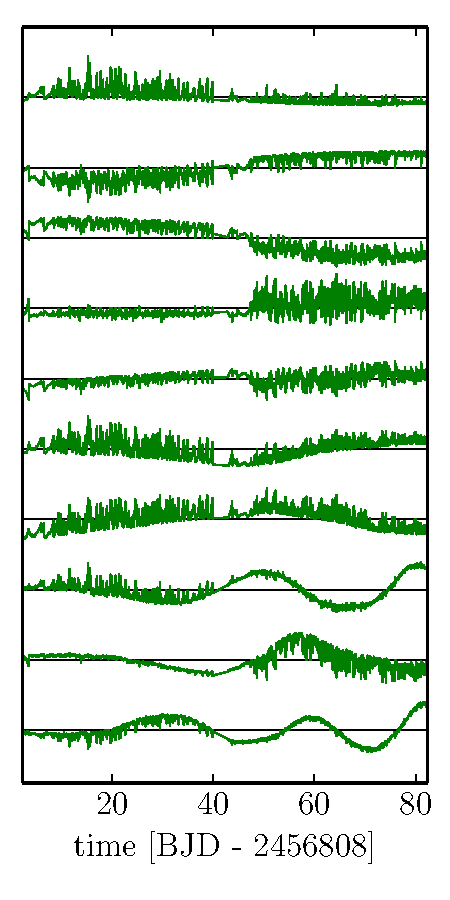
\includegraphics{figures/ketu/pca.pdf}
\end{center}
\caption{%
The top 10 eigen light curves (ELCs) generated by running principal component
analysis on all the aperture photometry from Campaign~1.
\figlabel{pca}}
\end{figure}


\section{Joint transit \& variability model}
\sectlabel{model}

The key insight in our transit search method that sets it apart from most
standard procedures is that no de-trending is necessary.
Instead, we can fit for the noise (or trends) and exoplanet signals
simultaneously.
This is theoretically appealing because it should be more sensitive to low
signal-to-noise transits \response{and similar methods have been shown to be
effective for finding transits in ground-based surveys \citep{Berta:2012}}.
The main motivation for this model is that the signal is never precisely
orthogonal to the systematics and any de-trending will over-fit.
This will, in turn, decrease the amplitude of the signal and distort its
shape.
In order to reduce these effects, most de-trending procedures use a very rigid
model for the systematics.
For \KT, this rigidity has been implemented by effectively asserting that
centroid measurements contain all of the information needed to describe the
trends \citep{Vanderburg:2014, Aigrain:2015, Crossfield:2015}.
In the \kepler\ pipeline, this is implemented by allowing only a small number
of PCA components to contribute to the fit in the \pdc\ procedure.
Instead, we will use a large number of ELCs---a very flexible model---and use
a simultaneous fitting and marginalization to avoid over-fitting.

Physically, the motivation for our model---and the \pdc\ model---is that every
star on the detector should be affected by the same set of systematic effects.
These are caused by things like pointing jitter, temperature variations, and
other sources of PSF modulation.
Each of these effects will be imprinted in the light curves of many stars with
varying amplitudes and signs as a result of the varying flat field and PSF.
Therefore, while it is hard to write down a physical generative model for the
systematics, building a data-driven model might be possible.
This intuition is also exploited by other methods that model the systematics
using only empirical centroids \citep{Vanderburg:2014, Armstrong:2014,
Aigrain:2015, Crossfield:2015}, but our more flexible model should capture a
wider range of effects, including those related to PSF and temperature.
For example, \Fig{corr} shows the application of our model---with 150
ELCs---to a light curve with no known transit signals and the precision is
excellent.

If we were to apply this systematics model alone (without a simultaneous fit
of the exoplanet transit model) to a light curve with transits, we would be at
risk of over-fitting and decreasing the amplitude of the signal.
\response{\Fig{overfitting} demonstrates this effect on a synthetic transit
injected into the light curve of a typical bright star.
The middle two panels in this Figure show the light curve de-trended using 10
and 150 ELCs respectively.
When only 10 ELCs are used, the measured transit depth is relatively robust
but this model is clearly not sufficient for removing the majority of the
systematic trends.
The model with 150 ELCs does an excellent job of removing the systematics but
it also distorts the transit shape and decreases the measured transit depth,
hence reducing the signal strength in the \project{BLS} spectrum
\citep{Kovacs:2002}.}

In our pipeline we simultaneously fit for the transit signal and the trends
using a rigid model for the signal and a relatively flexible model for the
systematic noise.
Specifically, we model the light curve as being generated by linear
combination of 150 ELCs and a ``box'' transit model at a specific period,
phase, and duration.
The mathematical details are given in \app{math}, but in summary, since the
model is linear, we can analytically compute the likelihood
function---conditioned on a specific period, phase, and duration---for the
depth \emph{marginalizing out the systematics model}.
The signal-to-noise of this depth measurement can then be used as a quality of
fit metric or candidate selection scalar.
This computation is expensive but, as described in the following \sectionname
s, it is possible to scale the method to a \KT-size dataset.
\response{The bottom panel of \Fig{overfitting} shows the application of this
joint transit--systematics model to the synthetic transit discussed
previously.
When the joint model is used, the correct transit depth is measured---the
transit is not distorted---but the systematics are also well-described by the
model.}

It is worth noting that this model can be equivalently thought of as a
(computationally expensive) generalization of the ``Box Least Squares''
\citep[\project{BLS};][]{Kovacs:2002} method to a more sophisticated
description of the noise and systematics.
Therefore, any existing search pipeline based on \project{BLS} could, in
theory, use this model as a drop-in replacement, although some modifications
might be required for computational tractability.

\response{%
The choice to use 150 basis functions is largely arbitrary and we make no
claims of optimality.
This value was chosen as a trade-off between the computational cost of the
search---the cost scales as the third power of the size of the basis---and the
predictive power of the model.
In some preliminary experiments, we found that using a larger basis did, as
expected, lead to a marginally higher sensitivity to small transit signals
but the gain wasn't sufficient to justify the added cost.
}

\begin{figure}[p]
\begin{center}
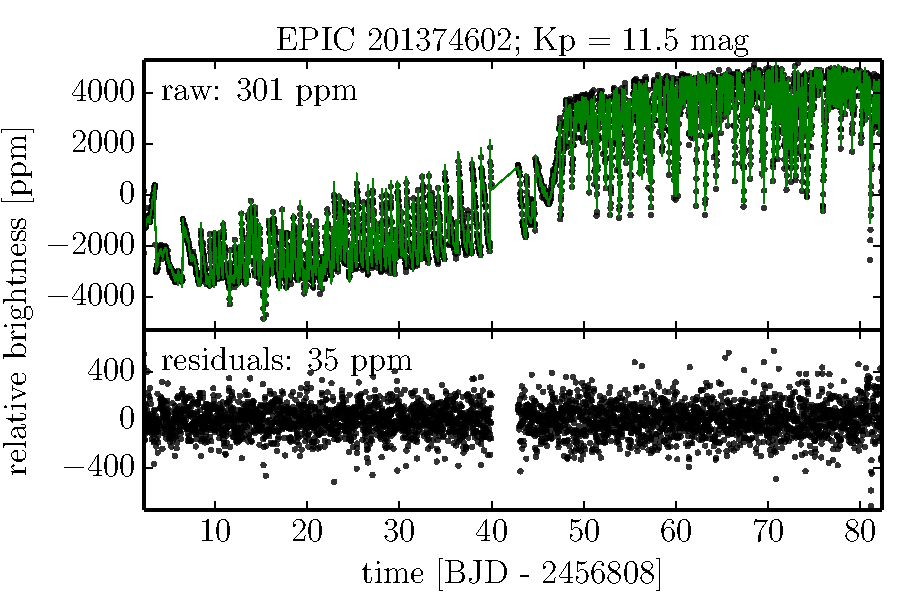
\includegraphics{figures/ketu/corr.pdf}
\end{center}
\caption{%
A demonstration of the ELC fit to the aperture photometry for EPIC 201374602.
\emph{Top:} The black points show the aperture photometry and the green line
is the maximum likelihood linear combination of ELCs.
The estimated 6-hour precision of the raw photometry is 264 ppm.
\emph{Bottom:} The points show the residuals of the data away from the ELC
prediction.
The 6-hour precision of this light curve is 31 ppm.
Note that although we show a ``de-trended'' light curve to give a qualitative
understanding of the model, this is not a product of the analysis.
In this search for transits, \emph{the data are never de-trended}.
\figlabel{corr}}
\end{figure}

\begin{figure}[p]
\begin{center}
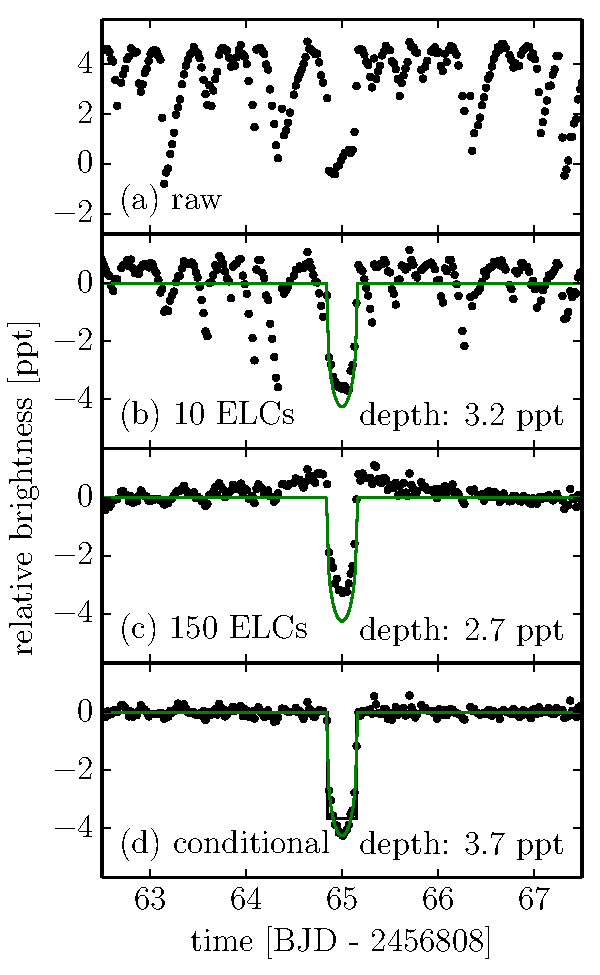
\includegraphics[width=0.5\textwidth]{figures/ketu/overfitting.pdf}
\end{center}
\caption{%
\response{%
A comparison between de-trending using different numbers of ELCs and a
simultaneous fit of the systematics and transit model.
\emph{(a)} The raw photometry for EPIC 201374602 with a synthetic transit
injected at 65 days. In all plots, the photometry is measured in
parts-per-thousand (ppt).
\emph{(b)} The black points show the photometry de-trended using a linear
combination of 10 ELCs and the green line shows the true transit model.
The maximum likelihood transit depth is computed following \project{BLS}
\citep{Kovacs:2002}.
While some of the systematics are removed by this model, there is still a lot
of residual noise.
\emph{(c)} The same plot as panel \emph{(b)} but using 150 ELCs to de-trend.
This model removes the majority of the systematics but also distorts the
transit and weakens the signal; it reduces the measured transit depth.
\emph{(d)} The final panel shows the results of simultaneously fitting for
the transit and the systematics using 150 ELCs.
The maximum likelihood depth is computed as described in \app{math}.
Like panel \emph{(c)}, this model removes most of the systematics but does
not distort the transit or reduce the measured transit depth.
}
\figlabel{overfitting}}
\end{figure}


\section{Search pipeline}
\sectlabel{search}

In principle, the search for transit signals simply requires evaluation of the
model described above on a fine three-dimensional grid in period, phase, and
duration, and then detection of high significance peaks in that space.
In practice, this is computationally intractable for any grids of the
required size and resolution.
Instead, we can compute the values on this grid approximately, but at very
high precision, using a two-step procedure that is much more efficient.

Specifically, we must evaluate the likelihood function for the light curve of
star $n$ given a period \period, reference transit time \phase, duration
\duration, \response{and depth \depth}
\begin{eqnarray}\eqlabel{full-likelihood}
p(\{\flux\}_n\,|\,\period,\,\phase,\,\duration,\,\depth) \quad.
\end{eqnarray}
We make the simplifying assumption that each transit enters this quantity
independently.
This is not true; as we change beliefs about each transit, we change beliefs
about the systematics model, which in turn affects the other transits.
However, this simplifying assumption
is approximately satisfied for all but the shortest
periods and leads to a huge computational advantage.
Under this assumption, this likelihood function can be rewritten as
\begin{eqnarray}\eqlabel{indtran}
p(\{\flux\}_n\,|\,\period,\,\phase,\,\duration,\,\depth) &=&
\prod_{m=1}^{M(\period,\,\phase)}
    p(\{\flux\}_n\,|\,\transittime_m(\period,\,\phase),\,\duration,\,
                    \depth)
\end{eqnarray}
where $\transittime_m(\period,\,\phase)$ is the time of the $m$-th
transit given the period $\period$ and reference time $\phase$, and
\response{$M(\period,\,\phase)$ is the total number of transits in the dataset
for the given \period\ and \phase}.
\Eq{indtran} can be efficiently computed for many periods and phases if we
first compute a set of likelihood functions for single transits on a grid
in $\transittime_l$ and duration $\duration_k$
\begin{eqnarray}\eqlabel{singletransit}
\left \{ p(\{\flux\}_n\,|\,\transittime_l,\,\duration_k,\,\depth)
\right\}_{l=1,\,k=1}^{L,\,K} \quad.
\end{eqnarray}
Then, we can use these results as a look-up table\response{---with
nearest-neighbor interpolation---}to approximately evaluate the full
likelihood in \eq{full-likelihood}.

In the remainder of this \sectionname, we give more details about each step of
the search procedure.
In summary, it breaks into three main steps: linear
search, periodic search, and vetting.
In the {\bf linear search} step, we evaluate the likelihood function in
\eq{singletransit} on a two-dimensional grid, coarse in transit duration
$\duration_k$ and fine in transit time $\transittime_m$.
Then in the {\bf periodic search} step, we use this two-dimensional grid to
approximately evaluate the likelihood (\eqalt{indtran}) for a
three-dimensional grid of periodic signals.
Then, we run a peak detection algorithm on this grid that discards signals
with substantially varying transit depths.
These transit candidates are then passed along for machine and human {\bf
vetting}.


\paragraph{Linear search}

The linear search requires hypothesizing a set of transit signals on a
two-dimensional grid in transit time and duration.
For each point in the grid, we use the model described in \sect{model} to
evaluate \emph{the likelihood function} for the transit depth at that time
and duration.
Since the model is linear, the likelihood function for the depth (marginalized
over the model of the systematics) is a Gaussian with analytic amplitude $L$,
mean $\bar{\depth}$, and variance $\delta\bar{\depth}^2$, all derived and given in
\app{math}.
In the linear search, we save these three numbers on a
two-dimensional grid of transit times $\transittime_l$ and durations
$\duration_k$.
The transit time grid spans the full length of Campaign~1 with half hour spacing
and we choose to only test three durations: 1.2, 2.4, and 4.8 hours.
\Fig{linear} shows the maximum likelihood transit depth $\bar{\depth}$ as a
function of transit time \transittime\ for the light curve of EPIC 201613023,
a transiting planet candidate with a period of 8.3~days.

\begin{figure}[p]
\begin{center}
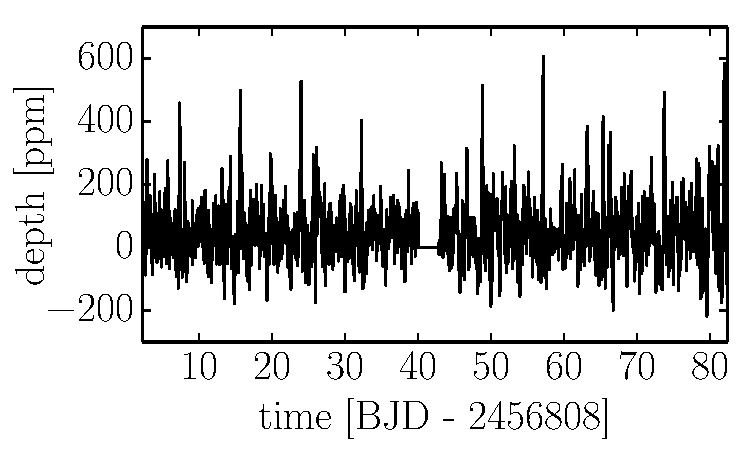
\includegraphics{figures/ketu/linear.pdf}
\end{center}
\caption{%
The maximum likelihood transit depth as a function of transit time as computed
in the linear search of the light curve of EPIC 201613023.
After the periodic search and vetting this target is found to have a planet
candidate with a period of 8.3~days.
The first transit occurs at 7.4~days on this plot.
\figlabel{linear}}
\end{figure}


\paragraph{Periodic search}

\response{%
In the period search step, the table of likelihood functions generated in the
linear search step are used to compute the likelihood of the periodic model
(\eqalt{indtran}) on a three dimensional grid in period \period, reference
time \phase, and duration \duration.
At each point in this grid, the likelihood function for each transit depth is
chosen as the nearest point calculated in the linear search.
If the time spacing of the linear search is sufficiently fine, this will give
a good approximation of the correct periodic likelihood.}
For each periodic model, we compute the likelihood of a model where the
transit depth varies between transits and the ``correct'' simpler model where
the transit depth is constant.
The variable depth likelihood is given by the product of amplitudes from the
initial search
\begin{eqnarray}
p_\mathrm{var}(\{\flux\}_n\,|\,\period,\,\phase,\,\duration) &=&
\prod_{m=1}^{M(\period,\,\phase)} L_m \quad.
\end{eqnarray}
Since the likelihood function for the depth at each transit time is known and
Gaussian, the likelihood function for the depth under the periodic model can
also be computed analytically; it is a product of Gaussians which itself is a
Gaussian
\begin{eqnarray}
p_\mathrm{const}(\{\flux\}_n\,|\,\period,\,\phase,\,\duration) &=&
\prod_{m=1}^{M(\period,\,\phase)}
    \frac{L_m}{\sqrt{2\,\pi\,{\delta\bar{\depth}_m}^2}}\,\exp \left(
        -\frac{[\depth - \bar{\depth}_m]^2}{2\,{\delta\bar{\depth}_m}^2}
    \right)
\end{eqnarray}
where the maximum likelihood depth, for the periodic model, is
\begin{eqnarray}\eqlabel{periodic-depth}
\depth &=& {\sigma_\depth}^2\,\sum_{m=1}^{M(\period,\,\phase)}
    \frac{\bar{\depth}_m}{{\delta\bar{\depth}_m}^2}
\end{eqnarray}
and the uncertainty is given by
\begin{eqnarray}\eqlabel{periodic-depth-uncert}
\frac{1}{{\sigma_\depth}^2} &=& \sum_{m=1}^{M(\period,\,\phase)}
    \frac{1}{{\delta\bar{\depth}_m}^2} \quad.
\end{eqnarray}
Note that this result has been \emph{marginalized} over the parameters of the
systematics model.
Therefore, this estimate of the uncertainty on the depth takes any
uncertainty that we have about the systematics into account.

In general, the variable depth model will \emph{always} get a higher
likelihood because it is more flexible.
Therefore, a formal model comparison is required to compete these two models
against each other on equal footing.
For computational simplicity and speed, we use the Bayesian Information
Criterion (BIC).
The traditional definition of the BIC is
\begin{eqnarray}
-\frac{1}{2}\,\BIC &=&
    \ln p(\{\flux\}_n\,|\,\period,\,\phase,\,\duration)
    - \frac{K}{2} \ln N
\end{eqnarray}
where the likelihood function is evaluated at the maximum, $K$ is an estimate
of the model complexity and $N$ is the effective sample size.
To emphasize that $K$ and $N$ are tuning parameters of the method, we
rewrite this equation as
\begin{eqnarray}
-\frac{1}{2}\,\BIC &=&
    \ln p(\{\flux\}_n\,|\,\period,\,\phase,\,\duration) -
        \frac{J\,\alpha}{2}
\end{eqnarray}
where $J$ is the number of allowed depths---one for the constant depth model
and the number of transits for the variable depth model---and $\alpha$ is
chosen heuristically.
For the K2 Campaign~1 dataset, we find that $\alpha \sim 1240$ leads to
reliable recovery of injected signals while still being fairly insensitive to
false signals.

To limit memory consumption, in the periodic search, we profile (or maximize)
over \phase\ and \duration\ subject to the constraint that
$\BIC_\mathrm{const} < \BIC_\mathrm{var}$ and requiring that the signal have
at least two observed transits.
This yields a one-dimensional spectrum of the signal-to-noise of the depth
measurement as a function of period using Equations~(\ref{eq:periodic-depth})
and (\ref{eq:periodic-depth-uncert}) to compute $\depth/\sigma_\depth$ at
each period.
The result is a generalization of the \project{BLS} frequency spectrum
\citep{Kovacs:2002} to a light curve model that includes both a transit and
the trends.
For example, \fig{periodic} shows the spectrum for a planet candidate
transiting EPIC 201613023.

After selecting the best candidate based on the signal-to-noise of the depth,
we mask out the sections of the linear search corresponding to these transits
and iterate the periodic search.
This permits us to find second transiting planets in light curves in which
we have already found a more prominent signal.
Under our assumption of independent transits, this masking procedure is
equivalent to removing the sections of data that have a transit caused by the
exoplanet that produces the highest peak.
For the purposes of this \paper, we iterate the periodic search until we find
three peaks for each light curve.
This will necessarily miss the smallest and longest period planets in systems
with more than three transiting planets but given the conservative vetting in
the next \sectionname, three peaks are sufficient to discover all the high
signal-to-noise transits.

\begin{figure}[p]
\begin{center}
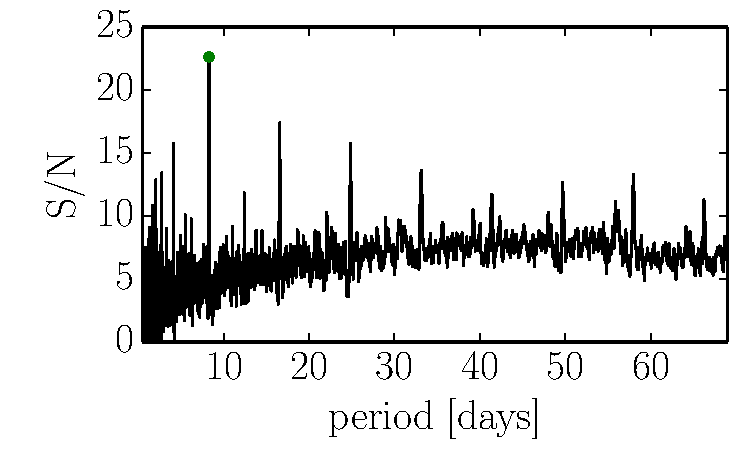
\includegraphics{figures/ketu/periodic.pdf}
\end{center}
\caption{%
The signal-to-noise spectrum as a function of period for the light curve of
EPIC 201613023.
This is the generalization of the \project{BLS} spectrum \citep{Kovacs:2002}
to this simultaneous model of the transit and the systematic trends.
To compute this spectrum, the results of the linear search (\fig{linear})
were used as described in \sect{search}.
The top peak (at a period of 8.3~days) is indicated with a green dot.
Iterating the periodic search found no other transit signals above the
signal-to-noise threshold.
\figlabel{periodic}}
\end{figure}



\paragraph{Initial candidate list}

The periodic search procedure returned three signals per target so this gave
an initial list of 65,109 candidates.
The vast majority of these signals are not induced by a transiting planet:
there are many false positives.
Therefore to reduce the search space, we estimate the signal-to-noise of each
candidate by comparing the peak height to a robust estimate of variance in
\BIC\ values across period.
This is not the same criterion used to select the initial three peaks but we
find that it produces a more complete and pure sample.
A cut in this quantity can reject most variable stars and low signal-to-noise
candidates that can't be reliably recovered from the data.
To minimize contamination from false alarms but maximize our sensitivity, we
choose a threshold of 15.
We also find that the signals with periods $\lesssim 4$ days are strongly
contaminated by false alarms.
This might be because of the fact that our independence assumption
(\eqalt{indtran}) breaks down at these short periods.
Therefore, we discard all signals with periods shorter than 4 days,
acknowledging this will cause us to miss some planets
\citep{Sanchis-Ojeda:2014}.
After these cuts, 741 candidates remain; we examine these signals by hand.
The full list of peaks and their relevant meta data is available online
at\footnote{\datareleaseurl}.


\paragraph{Hand vetting}

After our initial cuts on the candidate list, the majority of signals are
still false alarms mostly due to variable stars or single outlying data
points.
It should be possible to construct a more robust machine vetting algorithm
that discards these samples without missing real transits but for the purposes
of this \paper, we simply inspect the light curve for each of the 741
candidates \emph{by hand} to discard signals that are not convincing transits.
The results of this vetting can be seen online\footnote{\datareleaseurl}.

Although de-trended light curves are never used in the automated analysis of
the data, when conditioned on a specific set of transit parameters, the model
produces an estimate of what the light curve would look like in the absence
of systematic effects.
This prediction is one of the plots that we examine when vetting candidates
by hand.
For example, \fig{de-trended} shows the maximum likelihood light curve for
EPIC 201613023 evaluated at the candidate period, phase, duration, and depth.
Similarly, \fig{folded} shows the same prediction folded on the 8.3~day
period of this candidate.

After visually inspecting 741 signals, 101 candidate transits pass and are
selected as astrophysical events.
Many of these signals are due to ``false positives'' such as eclipsing binary
systems, either as the target star or as a background ``blend.'' We address
this effect in the following \sectionname, where we separate the list of
candidates into a list of astrophysical false positives and planet candidates.

\begin{figure}[p]
\begin{center}
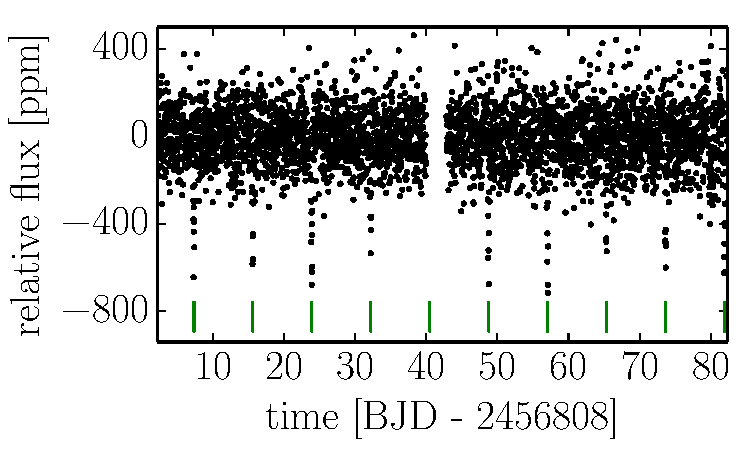
\includegraphics{figures/ketu/de-trended.pdf}
\end{center}
\caption{%
The maximum likelihood ``de-trended'' light curve for EPIC 201613023
evaluated at the planet candidate's period, phase, duration, and depth.
The transit times are indicated by the green ticks below the light curve.
This Figure is only generated for qualitative hand vetting and in the search
procedure, the model is always marginalized over any choices about the
systematic trends.
\figlabel{de-trended}}
\end{figure}

\begin{figure}[p]
\begin{center}
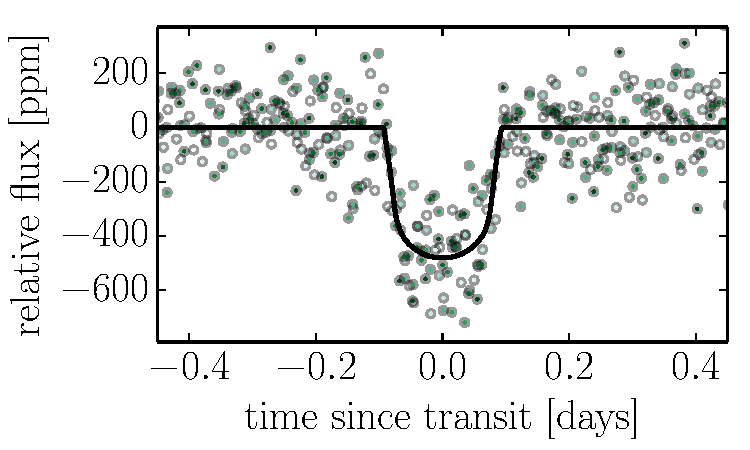
\includegraphics{figures/ketu/folded.pdf}
\end{center}
\caption{%
The maximum likelihood prediction for the light curve of EPIC 201613023 (see
also \fig{de-trended}) folded on the 8.3~day period of this planet candidate.
The points are color-coded by time and the median \emph{a posteriori} transit
model is overplotted as a black line.
\figlabel{folded}}
\end{figure}


\paragraph{Astrophysical false positives}

A major problem with any transit search is the potential confusion
between transiting planets and stellar eclipsing binaries (EBs).  Of
particular concern are grazing stellar eclipses or stellar eclipses
that contribute only a small fraction of the total light in a
photometric aperture, resulting in greatly diluted eclipse depths able
to mimic the signals of small planets.

Ground-based transit surveys have experienced false-positive rates
well over 50~percent.  For example, \citet{Latham:2009} reported eight
eclipsing binaries and one transiting planet among the sample of
transit candidates in one field of the Hungarian Automated Telescope
Network transit search.  In fact, the follow-up process to try to rule
out such astrophysical false positives is a large portion of the
effort that goes into a transit survey
\citep[e.g.,][]{Odonovan:2006,Almenara:2009,Poleski:2010}.

Despite this large fraction of astrophysical false positives in
ground-based surveys, the primary \kepler\ Mission saw a much lower
false positive rate of only 5-10\% \citep{Morton:2011, Fressin:2013},
primarily due to three major factors.  First, the superior precision
of the \kepler\ photometry enables detection of secondary stellar
eclipses, odd-even transit depth variations, and ellipsoidal
variations \citep{Batalha:2010} to a much lower level than
ground-based surveys. Second, the relatively small pixels and stable
pointing of the \kepler\ telescope has enabled the identification of
many spatially distinct blended eclipsing binaries by means of
detailed pixel-level analysis \citep{Bryson:2013} to identify shifts
in the center of light during transits.  And finally, \kepler\ is
sensitive to much smaller planets than ground-based surveys, and small
planets are much more common than the Jupiter-sized planets able to be
detected from the ground.

In \KT, the precision of the photometric tests used to vet for such
false positives  is lower and they must be applied
with care.  There are typically only a handful of transits, meaning
differences between ``odd'' and ``even'' transits must be large to
create a significant difference. Searching for ellipsoidal variations
is hindered by the short time baseline and the increased photometric
uncertainty in \KT\ data.  Centroid variations are feasible in
\KT\ but must be treated differently than in the original
\kepler\ mission where this effect was generally measured using
difference imaging \citep{Batalha:2010, Bryson:2013}.

To do first-pass vetting for blended EBs among our catalog of
planetary candidates, we test for significant centroid offsets using
the machinery that we have already established for modeling the
systematic trends in the data, inspired by the methods used to vet
\kepler\ candidates \citep{Bryson:2013}.  This is only an initial vetting step
and a more complete characterization of our catalog's reliability is
forthcoming (Montet, \etal\ in preparation).

To measure \emph{centroid offsets}, we start by empirically measuring the
pixel centroid time series for each candidate by modeling the pixels near the
peak as a two-dimensional quadratic and finding the maximum at each time.
This method has been shown to produce higher precision centroid measurements
than center-of-light estimates (Vakili \etal, in preparation).
\Fig{centroid} shows the measured $x$ and $y$ pixel coordinate traces for EPIC
201613023.
Much like the photometry, this signal is dominated by the rigid body motion
of the spacecraft and we can, in fact, model it identically.
In our analysis, we model the light curve as a linear
combination of ELCs and a simple box transit model at a given period, phase,
and duration (\eqalt{linear-model}).
Under this model, the maximum likelihood depth can be computed analytically.
If we apply \emph{exactly the same model} to the centroid trace, the ``depth''
that we compute becomes the centroid motion in transit in units of pixels.
Since the motions won't necessarily point in a consistent direction across
transits, we treat each transit independently and report the average offset
amplitude weighted by the precision of each measurement.
To compute the significance of a centroid offset, we bootstrap the offset
amplitude for models at the same period and duration but randomly oriented
phases.
If the centroid measured for the candidate transit is substantially larger
than the random realizations, we label the candidate as a false positive.
In practice, the precision of the centroid measurements isn't sufficient to
robustly reject many candidates, but two candidates---EPIC 201202105 and EPIC
201632708---have offsets 3-$\sigma$ above the median out-of-transit offset
amplitude so they are removed from the final catalog.
For example, \Fig{offsets} shows the in-transit centroid offset measured for
EPIC 201202105 and compares it to the distribution of out-of-transit offset
amplitudes.

A quick \emph{a priori} estimate of the background blended eclipsing
binary rate serves as a good sanity check.  A query to the TRILEGAL
\citep[TRIdimensional modeL of thE GALaxy,][]{Girardi:2005} galaxy
line-of-sight simulation software reveals that the typical density of
field stars along the line of sight to the Campaign 1 field is about
$7.8\times 10^{-4}$\,arcsec$^{-2}$.  This gives a probability of about
0.16 that a background star might be blended within a 8\,arcsec radius
(two pixels) from a target star.  Allowing that $\sim$10\% of stars
might host close binary companions within the period range accessible
by this survey, this gives a probability of 0.016 that a blended
binary star might be chance-aligned within two pixels of any given
target star.  Noting that the average number of planets per star with
periods less than 30 days is about 0.25 \citep{Fressin:2013}, we can
roughly estimate that we expect $<$10\% of our candidates to be caused
by nearby contaminating EBs.  This estimate suggests that such
astrophysical false positives should be rare in our sample, consistent
with our detection of only 2 candidates with clear centroid offsets.

\begin{figure}[p]
\begin{center}
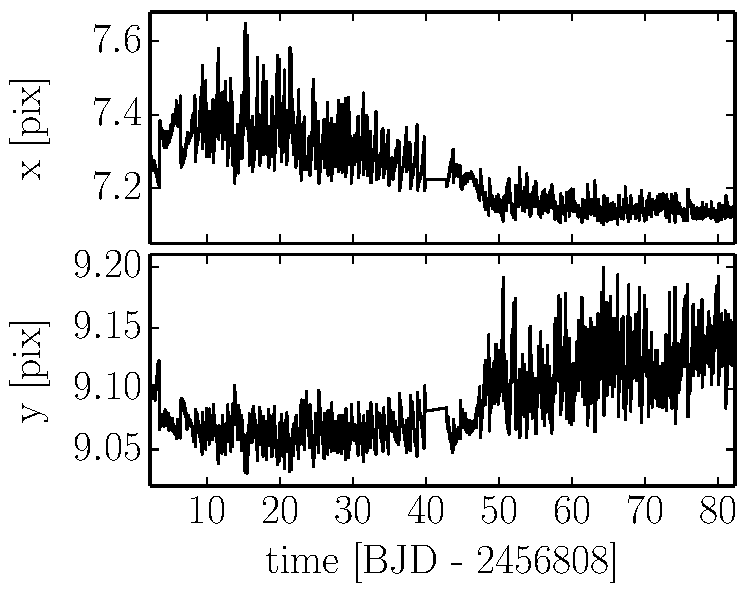
\includegraphics[width=0.4\textwidth]{figures/ketu/centroid.pdf}
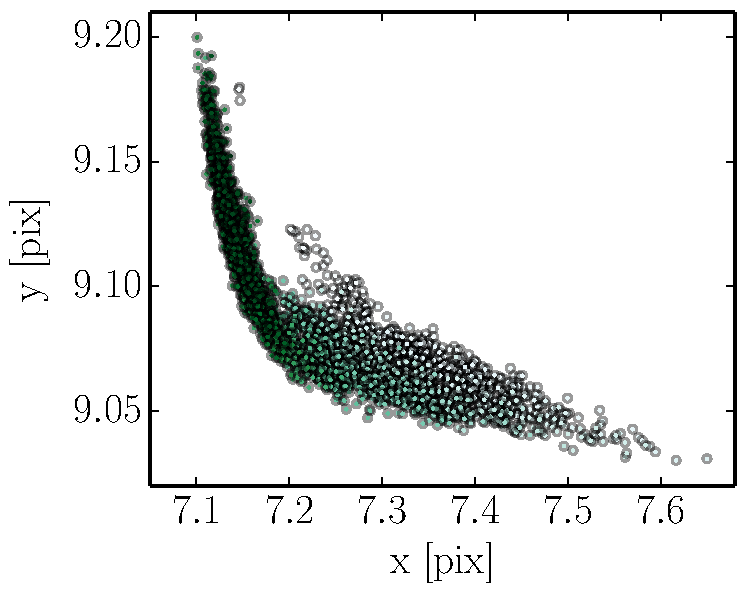
\includegraphics[width=0.4\textwidth]{figures/ketu/centroid-2.pdf}
\end{center}
\caption{%
The centroid motion for EPIC 201613023.
\emph{Left:} The measured $x$ and $y$ pixel coordinates as a function of time.
\emph{Right:} The pixel coordinates color-coded by time.
As identified by \citet{Vanderburg:2014}, the centroid motions fall in a
slowly time variable locus.
If the centroid coordinates in transit are inconsistent with the
out-of-transit motions, the candidate is likely to be an astrophysical false
positive.
\figlabel{centroid}}
\end{figure}

\begin{figure}[p]
\begin{center}
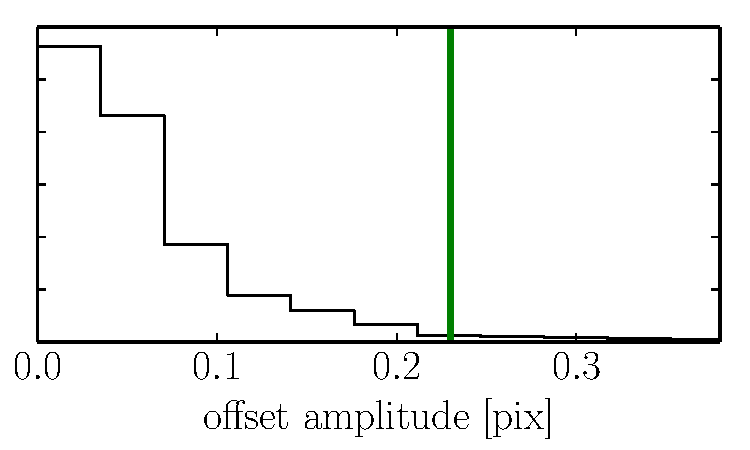
\includegraphics{figures/ketu/offsets.pdf}
\end{center}
\caption{%
The estimated in-transit centroid offset for EPIC 201202105 (green line)
compared to the distribution of 1000 centroid offests computed for randomly
assigned phases (black histogram).
The in-transit measurement is 3-$\sigma$ larger than the median out-of-transit
offset so it is rejected from the final catalog.
\figlabel{offsets}}
\end{figure}


\section{Performance}
\sectlabel{perform}

To test the performance and detection efficiency of our method, we conducted a
suite of injection and recovery tests, five per
star for all 21,703 target stars.
For each test, we inject the signal from a realistic planetary system into the
raw aperture photometry of a random target and run the resulting injected
light curve through the full pipeline (except the manual vetting).
If the search returns a planet candidate---passing all of the same cuts as we
apply in the main search (except the manual vetting)---with period and
reference transit time within 6~hours of the injected signal, we count that
injection as recovered.
The detection efficiency of the search is given approximately by the fraction
of recovered injections as a function of the relevant parameters.

To generate the synthetic signals, we use the following procedure:
\begin{enumerate}
{\item Draw the number of transiting planets based on the observed
multiplicity distribution of KOIs \citep{Burke:2014}.}
{\item Sample---from the distributions listed in
\tab{dist}---limb darkening parameters and, for each planet, an orbital
period, phase, radius ratio, impact parameter, eccentricity, and argument of
periapsis.}
{\item Based on the chosen physical parameters, simulate the light curve,
taking limb darkening and integration time into account \citep{Mandel:2002,
Kipping:2010}, and multiply it into the raw aperture photometry.}
\end{enumerate}
We then process these light curves using exactly the pipeline that we use for
the light curves without injections.
Finally, we test for recovery after applying the cuts in signal-to-noise and
period.
We should, of course, also vet the results of the injection tests by hand
to ensure that our measurements of detection efficiency aren't biased by the
hand-vetting
step but, since we chose to limit our sample to very high signal-to-noise
candidates, it seems unlikely that our hand vetting removed any true transit
signals.
Any estimates of the false alarm rate will, however, be affected by this
negligence but we leave a treatment of this for future work.

\figurename s~\figref{completeness} and~\figref{completeness-mag} show the
fraction of recovered signals as a function of the physical parameters of the
injection and the magnitude of the star in the \kepler\ bandpass as reported
in the Ecliptic Plane Input Catalog
(EPIC\footnote{\url{http://archive.stsci.edu/k2/epic.pdf}}).
As expected, the shallower transits at longer periods are recovered less
robustly and all signals become harder to detect for fainter stars.
It is worth noting that these \figurename s are projections (or
marginalizations) of a higher dimensional measurement of the recovery rate as
a function of all of the input parameters.
For example, this detection efficiency map is conditioned on our assumptions
about the eccentricity distribution of planets and it is marginalized over the
empirical distribution of stellar parameters.
It is possible to relax this assumption and apply different distributions by
re-weighting the simulations used to generate this figure.
Therefore, alongside this \paper, we publish the full list of injection
simulations\footnote{\datareleaseurl} to be used for population inference
(occurrence rate measurements).

\response{%
While we argue that the most relevant quantity to use to quantify the
performance of a transit search pipeline is the efficiency with which it
discovers transits, it is also useful to consider some other standard metrics.
In particular, while de-trended light curves are never used at any stage of
the analysis, our method does make a prediction for the systematics model and
we can measure the relative precision of the residuals away from this model.
These residuals are what would be used as de-trended light curves if that was
the goal.
\Fig{performance} shows, as a function of the \kepler\ magnitude reported in
the EPIC, the 6-hour CDPP \citep{Christiansen:2012} for each light curve after
subtracting the best fit linear combination of 150 ELCs.
}


\begin{figure}[p]
\begin{center}
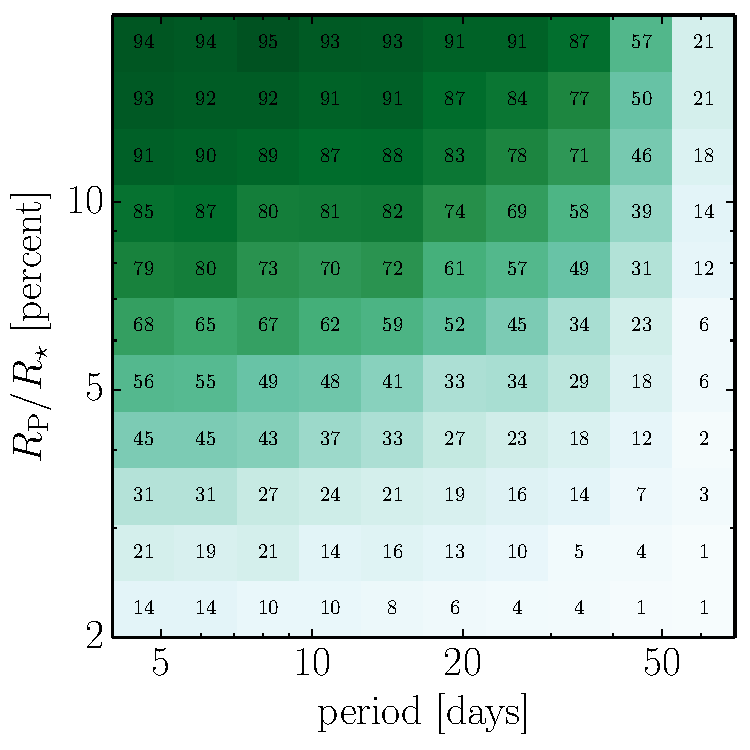
\includegraphics{figures/ketu/completeness.pdf}
\end{center}
\caption{%
The detection efficiency of the search procedure as a function of the
physical transit parameters computed empirically by
injecting synthetic transit signals into the raw light curves and measuring
the fraction that are successfully recovered.
These tests were performed on the entire set of stars so these numbers are
marginalized over all the stellar properties, including magnitude.
\figlabel{completeness}}
\end{figure}

\begin{figure}[p]
\begin{center}
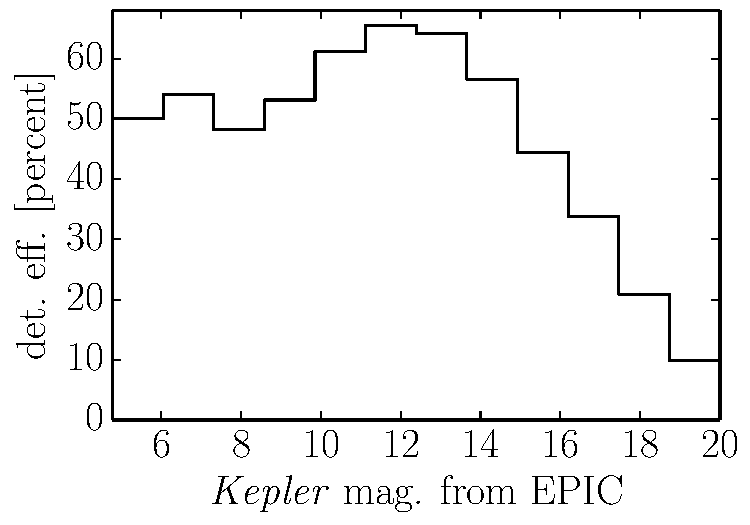
\includegraphics{figures/ketu/completeness-mag.pdf}
\end{center}
\caption{%
Like \fig{completeness}, the empirically measured detection efficiency of the
search procedure as a function of stellar magnitude as reported by the EPIC.
This never reaches 90~percent because these numbers are marginalized over the
range of physical parameters shown in \fig{completeness}.
Even for the brightest stars, the long period, small transits cannot be
detected.
\figlabel{completeness-mag}}
\end{figure}

\begin{figure}[p]
\begin{center}
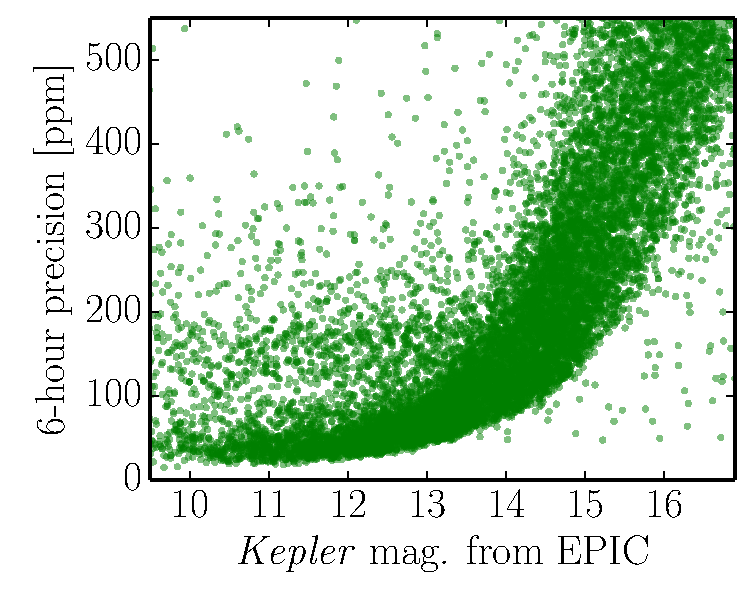
\includegraphics{figures/ketu/performance.pdf}
\end{center}
\caption{%
\response{%
The 6-hour CDPP \citep{Christiansen:2012} for each light curve in Campaign 1
after subtracting the best fit linear combination of 150 ELCs.
For each star, the precision is plotted as a function of the \kepler\
magnitude reported in the EPIC.
The ``outliers'' in the bottom right corner of the plot are caused by a
bright star within the photometric aperture and the points in the top left
corner of the plot are variable stars where the major trends in the light
curve are not caused by systematic effects, making the ELC model a bad fit.}
\figlabel{performance}}
\end{figure}

\begin{table}[p]
\begin{center}
\begin{tabular}{lcc}
\toprule
Parameter & Units & Distribution \\
\midrule

limb darkening parameters $q_1$ and $q_2$ & --- & $q \sim U(0,\,1)$ \\
orbital period \period & days & $\ln \period \sim U(\ln 0.5,\,\ln 70)$ \\
reference transit time \phase & days & $\phase \sim U(0,\,\period)$ \\
radius ratio $R_P/R_\star$ & --- & $\ln R_P/R_\star \sim U(\ln 0.02,\,\ln 0.2)$ \\
impact parameter \impact & --- & $\impact \sim U(0,\,1)$ \\
eccentricity \ecc & --- & $\ecc \sim \mathrm{Beta}(0.867,\,3.03)$ \\
argument of periapsis \pomega & --- & $\pomega \sim U(-\pi,\,\pi)$ \\

\bottomrule
\end{tabular}
\end{center}
\caption{%
The distribution of physical parameters for the injected signals.
The eccentricity distribution is based on \citet{Kipping:2013} and the
limb darkening parameterization is given by \citet{Kipping:2013a}.
\tablabel{dist}}
\end{table}



\section{Results}
\sectlabel{results}

Out of the 21,703 Campaign~1 light curves, our pipeline returns 741 signals
that pass the signal-to-noise and period cuts.
After hand vetting by the two first authors, this list is reduced to 101
convincing astrophysical transit candidates.
Of these, 36 signals---in 31 light curves---have no visible secondary
eclipse and are deemed planet candidates.
These planet candidates are listed in \tab{cand}.
The two candidates transiting EPIC 201367065 were previously published
\citep{Crossfield:2015} and the third planet in that system is found as the
third signal by our pipeline but it falls just below the signal-to-noise cut
so it is left out of the catalog for consistency.
This suggests that a less conservative cut in signal-to-noise and more
aggressive machine vetting could yield a much more complete catalog at smaller
radii and longer periods even with the existing dataset.

The remaining signals are caused by EBs with visible secondary eclipses.
In most cases, the search reports the secondary eclipse as a candidate and in
a few very high signal-to-noise cases, the period reported by the pipeline is
incorrect and multiple candidates correspond to the same transit.
It is important to note, however, that the choices made in the search were
heuristically tuned to find planets, not binaries, so our results are not
complete or exhaustive, especially at short orbital periods.
There are other methods specifically tuned to find EBs in \KT\
\citep[such as][]{Armstrong:2014, Armstrong:2015} and these catalogs contain
our full sample of EBs and more.

For the planet candidates, we perform a full physical transit fit to the light
curve.
To do this fit, we use Markov Chain Monte Carlo
\citep[MCMC;][]{Foreman-Mackey:2013} to
sample from the posterior probability for the stellar and planetary
parameters taking limb darkening and integration time into account.
In this fit, we continue to model the trends in the data as a linear
combination of the 150 ELCs but, at this point, we combine this with a
realistic light curve model \citep{Mandel:2002, Kipping:2013a}.
Even though we have no constraints on the stellar parameters, we also sample
over a large range in stellar mass and radius so that future measurements can
be applied by re-weighting the published samples.
In \tab{cand} we list the sample quantiles for the observable quantities and
the full chains are available electronically\footnote{\datareleaseurl}.
\fig{candidates} shows the observed distribution of planet candidates in the
catalog.

In a follow-up to this \paper, we will characterize the stars for each of the
candidates in detail but for now it's worth noting that many of the planet
candidates are orbiting stars selected for \KT\ as M-type stars.
If this rate remains robust after stellar characterization and if these
numbers are representative of the yields in upcoming \KT\ Campaigns, the \KT\
Mission will substantially increase the number of planets known to transit
cool stars.

\begin{figure}[p]
\begin{center}
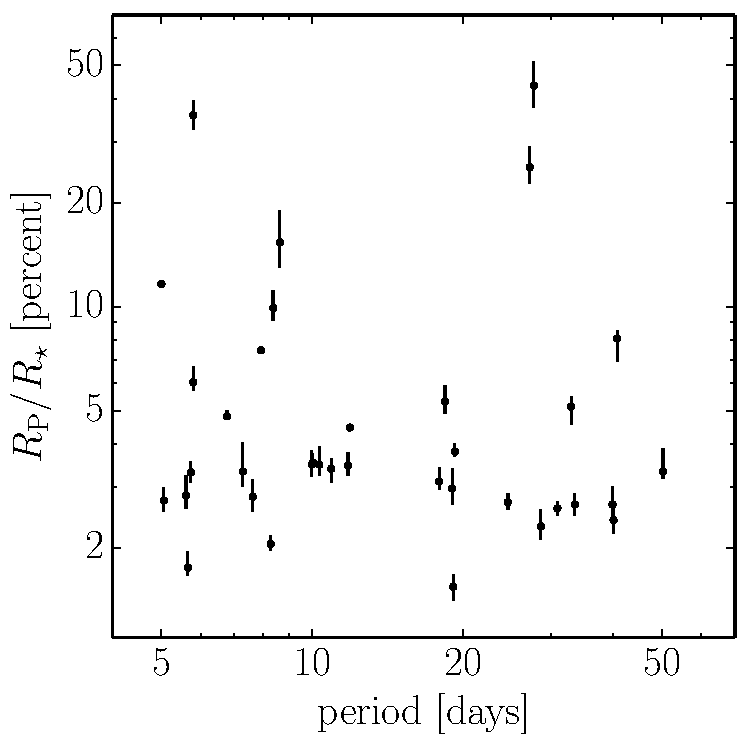
\includegraphics{figures/ketu/candidates.pdf}
\end{center}
\caption{%
The \emph{a posteriori} distribution of planet candidates in the catalog.
The error bars indicate the 0.16 and 0.84 posterior sample quantiles for the
radius ratios.
\figlabel{candidates}}
\end{figure}

\begin{table}[p]
\begin{center}
\small
\begin{tabular}{cccccc}
\toprule
EPIC & RA (J2000) & Dec (J2000) & \period\ [days] & $t_0$ [BJD-2456808] & $R_\mathrm{P} / R_\star$ \\
\midrule
201208431 & 174.745640 & -3.905585 & $10.0040_{-0.0016}^{+0.0018}$ & $7.5216_{-0.0090}^{+0.0098}$ & $0.0349_{-0.0026}^{+0.0034}$ \\
201257461 & 178.161109 & -3.094936 & $50.2677_{-0.0074}^{+0.0083}$ & $20.3735_{-0.0098}^{+0.0147}$ & $0.0334_{-0.0017}^{+0.0054}$ \\
201295312 & 174.011630 & -2.520881 & $5.6562_{-0.0007}^{+0.0007}$ & $3.7228_{-0.0091}^{+0.0086}$ & $0.0175_{-0.0009}^{+0.0020}$ \\
201338508 & 169.303502 & -1.877976 & $10.9328_{-0.0021}^{+0.0022}$ & $6.5967_{-0.0081}^{+0.0088}$ & $0.0339_{-0.0030}^{+0.0025}$ \\
201338508 & 169.303502 & -1.877976 & $5.7350_{-0.0006}^{+0.0006}$ & $0.8626_{-0.0055}^{+0.0054}$ & $0.0331_{-0.0023}^{+0.0025}$ \\
201367065 & 172.334949 & -1.454787 & $10.0542_{-0.0004}^{+0.0004}$ & $5.4186_{-0.0018}^{+0.0018}$ & $0.0354_{-0.0011}^{+0.0022}$ \\
201367065 & 172.334949 & -1.454787 & $24.6470_{-0.0016}^{+0.0014}$ & $4.2769_{-0.0029}^{+0.0030}$ & $0.0272_{-0.0013}^{+0.0016}$ \\
201384232 & 178.192260 & -1.198477 & $30.9375_{-0.0052}^{+0.0029}$ & $19.5035_{-0.0039}^{+0.0053}$ & $0.0260_{-0.0011}^{+0.0011}$ \\
201393098 & 167.093771 & -1.065755 & $28.6793_{-0.0116}^{+0.0105}$ & $16.6212_{-0.0177}^{+0.0305}$ & $0.0231_{-0.0020}^{+0.0028}$ \\
201403446 & 174.266344 & -0.907261 & $19.1535_{-0.0050}^{+0.0050}$ & $7.3437_{-0.0143}^{+0.0116}$ & $0.0154_{-0.0013}^{+0.0014}$ \\
201445392 & 169.793665 & -0.284375 & $10.3527_{-0.0011}^{+0.0011}$ & $5.6110_{-0.0051}^{+0.0047}$ & $0.0349_{-0.0025}^{+0.0045}$ \\
201445392 & 169.793665 & -0.284375 & $5.0644_{-0.0006}^{+0.0006}$ & $5.0690_{-0.0064}^{+0.0059}$ & $0.0274_{-0.0020}^{+0.0025}$ \\
201465501 & 176.264468 & 0.005301 & $18.4488_{-0.0015}^{+0.0015}$ & $14.6719_{-0.0032}^{+0.0035}$ & $0.0531_{-0.0039}^{+0.0061}$ \\
201505350 & 174.960319 & 0.603575 & $11.9069_{-0.0004}^{+0.0005}$ & $9.2764_{-0.0015}^{+0.0013}$ & $0.0446_{-0.0006}^{+0.0009}$ \\
201505350 & 174.960319 & 0.603575 & $7.9193_{-0.0001}^{+0.0001}$ & $5.3840_{-0.0008}^{+0.0006}$ & $0.0747_{-0.0013}^{+0.0016}$ \\
201546283 & 171.515165 & 1.230738 & $6.7713_{-0.0001}^{+0.0001}$ & $4.8453_{-0.0011}^{+0.0012}$ & $0.0481_{-0.0012}^{+0.0020}$ \\
201549860 & 170.103081 & 1.285956 & $5.6083_{-0.0006}^{+0.0005}$ & $4.1195_{-0.0047}^{+0.0045}$ & $0.0283_{-0.0023}^{+0.0041}$ \\
201555883 & 176.075940 & 1.375947 & $5.7966_{-0.0002}^{+0.0002}$ & $5.3173_{-0.0050}^{+0.0027}$ & $0.0604_{-0.0032}^{+0.0068}$ \\
201565013 & 176.992193 & 1.510249 & $8.6381_{-0.0002}^{+0.0003}$ & $3.4283_{-0.0015}^{+0.0016}$ & $0.1538_{-0.0243}^{+0.0355}$ \\
201569483 & 167.171299 & 1.577513 & $5.7969_{-0.0000}^{+0.0000}$ & $5.3130_{-0.0003}^{+0.0002}$ & $0.3587_{-0.0334}^{+0.0379}$ \\
201577035 & 172.121957 & 1.690636 & $19.3062_{-0.0013}^{+0.0013}$ & $11.5790_{-0.0027}^{+0.0025}$ & $0.0380_{-0.0012}^{+0.0023}$ \\
201596316 & 169.042002 & 1.986840 & $39.8415_{-0.0155}^{+0.0136}$ & $21.8572_{-0.0101}^{+0.0120}$ & $0.0267_{-0.0022}^{+0.0034}$ \\
201613023 & 173.192036 & 2.244884 & $8.2818_{-0.0007}^{+0.0006}$ & $7.3752_{-0.0052}^{+0.0055}$ & $0.0205_{-0.0008}^{+0.0012}$ \\
201617985 & 179.491659 & 2.321476 & $7.2823_{-0.0008}^{+0.0007}$ & $4.6337_{-0.0050}^{+0.0050}$ & $0.0333_{-0.0032}^{+0.0072}$ \\
201629650 & 170.155528 & 2.502696 & $40.0492_{-0.0259}^{+0.0186}$ & $4.5363_{-0.0172}^{+0.0202}$ & $0.0241_{-0.0020}^{+0.0025}$ \\
201635569 & 178.057026 & 2.594245 & $8.3681_{-0.0002}^{+0.0002}$ & $3.4514_{-0.0014}^{+0.0015}$ & $0.0991_{-0.0078}^{+0.0120}$ \\
201649426 & 177.234262 & 2.807619 & $27.7704_{-0.0001}^{+0.0001}$ & $13.3476_{-0.0002}^{+0.0001}$ & $0.4365_{-0.0583}^{+0.0777}$ \\
201702477 & 175.240794 & 3.681584 & $40.7365_{-0.0025}^{+0.0026}$ & $3.5451_{-0.0025}^{+0.0026}$ & $0.0808_{-0.0114}^{+0.0043}$ \\
201736247 & 178.110797 & 4.254747 & $11.8106_{-0.0019}^{+0.0016}$ & $3.8483_{-0.0071}^{+0.0093}$ & $0.0347_{-0.0024}^{+0.0030}$ \\
201754305 & 175.097258 & 4.557340 & $19.0726_{-0.0049}^{+0.0048}$ & $1.4893_{-0.0133}^{+0.0128}$ & $0.0297_{-0.0030}^{+0.0042}$ \\
201754305 & 175.097258 & 4.557340 & $7.6202_{-0.0011}^{+0.0012}$ & $3.6813_{-0.0057}^{+0.0061}$ & $0.0281_{-0.0026}^{+0.0034}$ \\
201779067 & 168.542699 & 4.988131 & $27.2429_{-0.0001}^{+0.0001}$ & $12.2599_{-0.0003}^{+0.0002}$ & $0.2535_{-0.0259}^{+0.0369}$ \\
201828749 & 175.654342 & 5.894323 & $33.5093_{-0.0018}^{+0.0023}$ & $5.1554_{-0.0032}^{+0.0037}$ & $0.0267_{-0.0020}^{+0.0021}$ \\
201855371 & 178.329775 & 6.412261 & $17.9715_{-0.0017}^{+0.0015}$ & $9.9412_{-0.0038}^{+0.0033}$ & $0.0311_{-0.0017}^{+0.0030}$ \\
201912552 & 172.560460 & 7.588391 & $32.9410_{-0.0032}^{+0.0039}$ & $28.1834_{-0.0105}^{+0.0057}$ & $0.0513_{-0.0056}^{+0.0035}$ \\
201929294 & 174.656969 & 7.959611 & $5.0084_{-0.0001}^{+0.0001}$ & $4.5703_{-0.0012}^{+0.0022}$ & $0.1163_{-0.0014}^{+0.0011}$ \\
\bottomrule
\end{tabular}

\end{center}
\caption{%
The catalog of planet candidates and their observable properties.
These values and their uncertainties are derived from MCMC samplings and the
numbers are computed as the 0.16, 0.5, and 0.84 posterior sample quantiles.
The coordinates are retrieved directly from the EPIC.
\tablabel{cand}}
\end{table}

\section{Discussion}

We have searched the \KT\ Campaign~1 data set for exoplanet transit signals.
Our search is novel because it includes a very flexible systematics model,
which is fit simultaneously with the exoplanet signals of interest (and
marginalized out).
By this method, we find 36 transiting exoplanets, which we have vetted by both
automatically and manually and characterized by probabilistic modeling.
The candidates are listed in \tab{cand} and posterior distributions of planet
candidate properties are available\footnote{\datareleaseurl}.

The flexible systematics model we employ is a 150-parameter linear combination
of PCA components derived from the full set of 21,703 stellar light curves.
That is, it presumes that the systematics afflicting each star are shared in
some way across other stars.
It is our belief---although not a strict assumption of our model---that these
systematics are caused primarily by pointing drifts, or movements of the
pixels in the focal plane relative to the stars.
In principle, if the systematics \emph{are} dominated by pointing issues, the
systematics model could require only three parameters---three Euler
angles---not 150 amplitudes.
However, because (as the pointing drifts) each star sees it's own unique
local patch of flat-field variations, the mapping from pointing drifts to
brightness variations can be extremely non-linear.
Furthermore, because when the pointing is moving fast there is a smearing of
the point-spread function, there are effects keyed to the time derivative of
the Euler angles as well.
The large number (150) of linear coefficients gives the linear model the
freedom to model complex non-linear behavior; we are trading off parsimony
in parameters with the enormous computational advantages of maintaining
linearity (and therefore also convexity).
The computational advantages of the linear model are three-fold:
Convexity obviates searching in parameter space for alternative modes;
linear least-squares optimization can be performed with simple linear algebra;
given Gaussian uncertainties and uninformative priors, marginalizations over
the linear parameters also reduces to pure linear algebra.

The goal of this \paper\ was to get exoplanet candidates out of the
\KT\ pixel-level data, it was \emph{not} to generate light curves.
That is, both the search phase and the characterization phase of the method
are approximations to computations of a likelihood function for the pixel
data telemetered down from the satellite.
We did not generate ``corrected'' or ``pre-search conditioned'' light-curves
at any stage; we simultaneously fit systematics and the signals of interest
to the raw data.
For this reason, there is no sense in which this method ever really
produces corrected light curves.
% For us, a systematics-corrected light curve is not really a thing.

In this work, we are agnostic about fundamental properties of the host stars.
The only assumptions we make are that the star targeted by the \KT\
team is truly the planet host, and that there is no dilution by other stars in
any aperture.
As a result, these posterior distributions reflect the maximum possible
uncertainty in parameters such as the planet radius, which depend sensitively
on properties of the host star.
To use these distributions to characterize the properties of specific systems,
one could re-weight our samples using a measurement of the inferred stellar
properties.

This project does not live in isolation and this is certainly not the last
time the \KT\ data will be searched!
There are other teams searching the \KT\ light curves for transiting planets
(A.~Vanderburg, private comm.) and they are likely to find some planets that
we did not and vice versa.
We make many heuristic choices and short-cuts in this search.
For example, the choice to work at 150 principal components was based on
computational feasibility and qualitative tests on a handful of light curves
instead of any real model selection or utility optimization.

Another major limitation is that, in principle, the systematics model is
designed to describe spacecraft-induced trends, but not intrinsic stellar
variability.
In practice, the method can still find planets around variable stars but a
more sophisticated model should be more robust in this case.
One appealing option would be to model the systematics as a Gaussian Process
where the input parameters are both time and the same 150 ELCs.
Interestingly, while this model isn't linear, the search and marginalization
can still be executed efficiently---using optimized linear algebra algorithms
\citep[][Foreman-Mackey et al.\ in preparation]{Ambikasaran:2014}---inside the
search loop.

Additionally, while we apply this systematics model simultaneously with a
transiting planet model to search for planet candidates, this scheme is
not restricted to planet searches.
Any astrophysical event that could be observed in the \KT\ data could be
searched for in the same way.
By modeling a set of ELCs with any arbitrary data model, events in the \KT\
data that appear similar to that data model could be identified.
Such a technique may be useful in searching for astrophysical events such as
ellipsoidal variations induced by orbiting companions,
stellar activity,
microlensing events, especially in the upcoming Campaign 9,
or
active galactic nuclei variability.



A substantial caveat to the reliability of all existing transiting exoplanet
searches is that they all include human intervention.
This makes quantifying the false alarm rate of these catalogs complicated.
There has been some work on automated vetting algorithms using supervised
classification algorithms \citep{McCauliff:2014, Jenkins:2014} but these
methods rely on hand classified examples for training and the performance is
not yet competitive with human classification.

The catalog of planet candidates presented here includes only planets with
periods longer than 4 days and at least two transits in the \KT\ Campaign~1
footprint.
This means that we are necessarily missing many planets with orbital periods
outside  this range.
In particular, planets with a single transit in the dataset must be
abundant.
These candidates are the most relevant for the study of planetary system
formation and for statistical inference of the distribution of habitable zone
exoplanets.
What's more, given the observing strategy for \tess, where each field will
only be contiguously observed for one month at a time, methods for finding and
characterizing planets with a single transit are vital and the new \KT\ light
curves are a perfect test bed.

As a supplement to this \paper, we make all the results, data products, and
MCMC chains available at \datareleaseurl.
The \LaTeX\ source for this \paper, complete with the full revision history,
is available at \url{http://github.com/dfm/k2-paper} and the pipeline
implementation is available at \url{http://github.com/dfm/ketu} under the MIT
open-source software license.
This code and a lot of computation time are all that is needed to reproduce
the \figurename s in this \paper.

\section{Appendix: Mathematical model}
\sectlabel{math}

We model the raw aperture photometry as a linear combination of 150 ELCs and
a transit model.
Formally, this can be written for the light curve of the $k$-th star as
\begin{eqnarray}\eqlabel{linear-model}
\bvec{f}_k &=& \bvec{A}\,\bvec{w}_k + \mathrm{noise}
\end{eqnarray}
where
\begin{eqnarray}
\bvec{f}_k &=& \left (\begin{array}{cccc}
    f_{k,1} & f_{k,2} & \cdots & f_{k,N}
\end{array}\right )^\T
\end{eqnarray}
is the list aperture fluxes for star $k$ observed at $N$ times
\begin{eqnarray}
\bvec{t} &=& \left (\begin{array}{cccc}
    t_{1} & t_{2} & \cdots & t_{N}
\end{array}\right )^\T \quad.
\end{eqnarray}
In \eq{linear-model}, the design matrix is given by
\begin{eqnarray}
\bvec{A} &=& \left (\begin{array}{cccccc}
    x_{1,1} & x_{2,1} & \cdots & x_{150,1} & 1 & m_\bvec{\theta}(t_1) \\
    x_{1,2} & x_{2,2} & \cdots & x_{150,2} & 1 & m_\bvec{\theta}(t_2) \\
    && \vdots &&&\\
    x_{1,N} & x_{2,N} & \cdots & x_{150,N} & 1 & m_\bvec{\theta}(t_N)
\end{array}\right )
\end{eqnarray}
where the $x_{j,n}$ are the basis ELCs---with the index $j$ running over
components and the index $n$ running over time---and $m_\bvec{\theta}(t)$ is
the transit model
\begin{eqnarray}
m_\bvec{\theta}(t) &=& \left\{\begin{array}{cl}
-1 & \mathrm{if\,}t\,\mathrm{in\,transit} \\
0 & \mathrm{otherwise}
\end{array}\right.
\end{eqnarray}
parameterized by a period, phase, and transit duration (these parameters are
denoted by \bvec{\theta}).

Assuming that the uncertainties on $\bvec{f}_k$ are Gaussian and constant,
the maximum likelihood solution for \bvec{w} is
\begin{eqnarray}
{\bvec{w}_k}^* &\gets& \left( \bvec{A}^\T\,\bvec{A} \right)^{-1}\,
                       \bvec{A}^\T\,\bvec{f}_k
\end{eqnarray}
and the marginalized likelihood function for the transit depth is a Gaussian
with the mean given by the last element of ${\bvec{w}_k}^*$ and the variance
given by the lower-right element of the matrix
\begin{eqnarray}
{\bvec{\delta w}_k}^2 &\gets& {\sigma_k}^2 \,
            \left( \bvec{A}^\T\,\bvec{A} \right)^{-1}
\end{eqnarray}
where $\sigma_k$ is the uncertainty on $\bvec{f}_k$.
The amplitude of this Gaussian is given by
\begin{eqnarray}\eqlabel{depth-likelihood}
\mathcal{L}_k &=& \frac{1}{(2\,\pi\,{\sigma_k}^2)^{N/2}}\,\exp\left(
-\frac{1}{2\,{\sigma_k}^2}\,
\left| \bvec{f}_k - \bvec{A}\,{\bvec{w}_k}^* \right|^2
\right)
\end{eqnarray}
evaluated at the maximum likelihood value ${\bvec{w}_k}^*$.

\section{Chapter Acknowledgements}

It is a pleasure to thank
Eric Agol (UW),
Ruth Angus (Oxford),
Tom Barclay (Ames),
Zach Berta-Thompson (MIT),
Daniel Bramich (QEERI, Qatar),
G\'eza Kov\'acs (Konkoly Observatory),
Laura Kreidberg (Chicago),
Erik Petigura (Berkeley),
Roberto Sanchis Ojeda (Berkeley),
and
Andrew Vanderburg (Harvard)
for helpful contributions to the ideas and code presented here.
DFM, DWH, and DW were partially supported by the National Science Foundation
(grant IIS-1124794),
the National Aeronautics and Space Administration
(grant NNX12AI50G), and the Moore--Sloan Data Science Environment at NYU.
BTM was supported by a National Science Foundation Graduate Research
Fellowship (grant DGE‐1144469).

This research made use of the NASA \project{Astrophysics Data System} and the
NASA Exoplanet Archive.
The Archive is operated by the California Institute of Technology, under
contract with NASA under the Exoplanet Exploration Program.
This \paper\ includes data collected by the \kepler\ mission. Funding for the
\kepler\ mission is provided by the NASA Science Mission directorate.
We are grateful to the entire \kepler\ team, past and present.
Their tireless efforts were all essential to the tremendous success of the mission
and the successes of \KT, present and future.
These data were obtained from the Mikulski Archive for Space Telescopes
(MAST).
STScI is operated by the Association of Universities for Research in
Astronomy, Inc., under NASA contract NAS5-26555.
Support for MAST is provided by the NASA Office of Space Science via grant
NNX13AC07G and by other grants and contracts.


% Conclusion
\chapter*{Conclusion}\addcontentsline{toc}{chapter}{Conclusion}
\chapter*{Conclusion}\addcontentsline{toc}{chapter}{Conclusion}

This dissertation concerns the use of probabilistic \pz\ estimates in inference (\Chap{chippr}) and more generically (\Chap{qp}), as well as the evaluation of the performance of \pzpdf s (\Chap{pzdc1}).
\aim{Expand this into a one-paragraph outline of all the chapters.}

\aim{Add a one-paragraph synopsis of each chapter including conclusions and what to do next, emphasizing the context of the problem and the scope of the results in the chapter.}

\aim{Summarize my overall research program, how this work fits into the field as a whole, what broadly remains to be done, and my vision for where the field is going.
\begin{itemize}
	\item use every part of the animal, don't throw away data
	\item must be careful and correct, or we will only get out what we put in
	\item how we make decisions about what's good and what's bad makes a difference, must \textit{design} metrics appropriate to our goals even when inconvenient
\end{itemize}}











% %%%%% Appendices start %%%%%%%%%%%%%%%%
% %% Comment out the following line if your thesis has no appendix
% \appendix
% \chapter{One more comment\label{chap:append}}

This is an appendix.

% %% Note: If your thesis has more than one appendix, NYU requires a "list of
% %% appendices" page before the body of the thesis. I don't provide the tools
% %% to create that here, so you're on your own for that one... Sorry.
% %\input{app2}

%%%% Bibliography %%%%%%%%%%%%%%%
\clearpage
\addcontentsline{toc}{chapter}{Bibliography}
\bibliography{thesis,lsstdesc,zPDF,pzdc1}


\end{document}
